\documentclass[journal]{IEEEtran}

\hyphenation{op-tical net-works semi-conduc-tor}
\usepackage{graphicx}
\graphicspath{{figures/}}
\usepackage{algorithm}
\usepackage{algorithmic}
\usepackage{amsmath}
\usepackage{booktabs}
\usepackage{cite}
\usepackage{bm}
\usepackage{amsfonts}
\usepackage{xcolor}
\usepackage[labelfont=bf]{caption}
\usepackage{subcaption}
\usepackage{float}
\usepackage{multirow}
\usepackage[hidelinks]{hyperref}
\usepackage{orcidlink}
\newcommand{\rev}[1]{\textcolor{blue}{#1}}
\newcommand{\newrev}[1]{\textcolor{red}{#1}}
\renewcommand{\thesubfigure}{\alph{subfigure}} 

\begin{document}

\title{Multi-Balancing-Agent Reinforcement Learning for Charging Control of Lithium-ion Batteries}


\author{%
        Xuanyi~Li\,\orcidlink{0009-0009-9775-1612},
        Tao Kuang\,\orcidlink{0009-0000-5283-032X},
        Zihao~Zheng,
        Bing-Chuan~Wang\,\orcidlink{0000-0002-0234-2843},~\IEEEmembership{Senior Member,~IEEE,}
        Biao Luo,~\IEEEmembership{Senior Member,~IEEE}
        and Zhongmei Li,~\IEEEmembership{Member,~IEEE}%
\thanks{{\emph{(Xuanyi Li and Tao Kuang are co-first authors.)}}
        Xuanyi Li, Tao Kuang, Zihao Zheng, Bing-Chuan Wang, and Biao Luo are with the School of Automation, Central South University, Changsha 410083, China (e-mail: 8207240609@csu.edu.cn; bingcwang@csu.edu.cn; biao.luo@csu.edu.cn).

Zhongmei Li is with the Key Laboratory of Smart Manufacturing in Energy Chemical Process, Ministry of Education, East China University of Science and Technology, Shanghai 200237, China (e-mail: zhongmeili@ecust.edu.cn).
}
}

\maketitle
\begin{abstract}
Abstract—Lithium-ion batteries have been widely used in electric vehicles and energy-storage systems because of their high energy density, long cycle life, and low self-discharge rate. However, cell-to-cell inconsistencies within battery packs can degrade charging efficiency, usable capacity, and safety, making fast charging and state-of-charge (SOC) balancing important for battery-pack operation. Conventional charging balancing methods typically rely on balancing algorithms combined with dedicated equalization topologies to redistribute charge or energy among cells. However, these approaches introduce additional energy-transfer or dissipation paths, resulting in energy losses or increased system complexity, while the possibility of SOC imbalance re-emerging during subsequent charging is often overlooked.

To address these limitations, this paper proposes a multi-balancing-agent reinforcement learning (MBA-RL) framework for charging control without a dedicated equalization topology. In MBA-RL, each agent regulates the charging current of one cell, while cooperating with the other agents to coordinate fast charging and pack-level SOC balancing. A model-based safety-constrained execution mechanism further screens the requested charging currents according to voltage, temperature, and SOC constraints before execution. The framework uses nonnegative charging-current commands and therefore avoids discharging high-SOC cells.

Experimental results over 60 evaluations covering 12 unseen initial-SOC conditions and five independent training runs show that MBA-RL reduces accumulated SOC imbalance by 12.65% and 10.82% compared with shared independent Q-learning and centralized deep Q-learning, respectively. The proposed safety-constrained execution mechanism satisfies the sampled limits in all 52 safety tests and, when incorporated into training, enables all 52 tests to reach the charging objective.
\end{abstract}
\vspace{-0.55\baselineskip}
\begin{IEEEkeywords}
Charging control, SOC balancing, lithium-ion battery, multi-agent reinforcement learning
\end{IEEEkeywords}

\IEEEpeerreviewmaketitle

\section{Introduction}

\IEEEPARstart{L}{ithium-ion} batteries have been extensively adopted in the electric vehicle (EV) industry due to their environment-friendly nature, high energy density, low self-discharge rate, and long cycle life \cite{1, 2}. However, individual lithium-ion batteries are inherently limited in meeting the high voltage and capacity demands required by EVs \cite{3, 4}. As a result, practical energy storage systems are composed of hundreds to thousands of individual battery cells. However, inevitable inconsistencies in manufacturing and operational conditions introduce variations in internal states and lifespan across battery cells, which can significantly compromise a battery pack’s overall capacity, charging efficiency, and durability while also increasing safety risks \cite{5, 6}. Therefore, it is crucial to formulate an efficient and practical charging equalization strategy that reduces charging time under safety constraints while ensuring inter-cell balance within the battery pack. To achieve this objective, researchers have developed numerous equalization strategies. Most of these strategies employ a framework that combines equalization topologies with balancing algorithms, where the balancing algorithm regulates the topology structure to achieve the redistribution of charge and energy within the battery pack \cite{7, 8}. Different balancing algorithms applied to the same equalization topology can yield varying results, and vice versa. A reasonable equalization strategy should strike a balance between these two aspects, taking into account the specific requirements of the application \cite{ma2024two}. A detailed overview of the framework is provided as follows.

\noindent\textit{Equalization topologies:} The equalization topologies can be categorized into active equalization topologies and passive equalization topologies. The active equalization topologies involve redistributing excess charge from high-energy cells to those with lower energy levels via switched capacitors, inductors \cite{9}, transformers \cite{10}, or DC-DC converters \cite{11}, thereby facilitating an efficient discharging process for high-energy cells while simultaneously charging low-energy cells. Despite the higher energy utilization efficiency offered by active balancing, designing an effective equalization topology becomes increasingly intricate when managing a large number of cells configured in both series and parallel arrangements. This significantly increases the complexity of the system and the associated design costs. Passive equalization topologies achieve charging equalization by employing discharge resistors connected in parallel with the cells within the battery pack \cite{12}. These resistors serve as a channel for high-energy cells to dissipate excess charge, with the energy being converted into heat during the process. Although the design of passive balancing is relatively straightforward, the dissipation of energy through resistors substantially reduces energy efficiency. \newrev{Thus, conventional active and passive equalization require additional energy-transfer or dissipation paths, introducing conversion losses or topology complexity.}

\noindent\textit{Balancing algorithms:} Traditional balancing algorithms are typically based on constant current-constant voltage (CC-CV) methods to achieve voltage or SOC balancing among battery cells. Aizpuru {\it et al.} \cite{13} integrated the CC-CV method with single-cell experimental data to construct a passive balancing system. Hoque {\it et al.} \cite{14} applied particle swarm optimization (PSO) to optimize the CC-CV balancing controller, aiming to improve balancing performance. Although CC-CV based balancing algorithms are straightforward to design, they fail to consider temperature variations within the battery pack and rely on overly conservative constraints to mitigate safety risks. With the advancement of control theory, an increasing number of studies have combined control theory with charging equalization topologies. In \cite{15}, a balancing algorithm employing fuzzy logic control was proposed to adaptively manage the equalization process for lithium-ion batteries. Fan {\it et al.} \cite{16} introduced a fast-balancing strategy based on model predictive control to resolve the issue of imbalance among individual cells in lithium-ion battery packs. While these approaches can enhance the precision and efficiency of charging equalization, they still fail to adapt to dynamic changes in battery parameters during the charging process. To address the aforementioned issues, Yang {\it et al.} \cite{17} presented a balancing awareness charging control framework based on deep reinforcement learning (DRL). In \cite{18}, a DRL-based controller was introduced for active equalization of redundant battery systems. These approaches leverage DRL’s adaptability to dynamic environments and its strong exploration capabilities to determine the optimal charging policy. Nevertheless, the previously mentioned DRL methods exhibit several issues: 1) depending on an equalization topology to enable charge and energy redistribution among cells, which compromises both charging efficiency and precision; 2) overlooking the possibility that, despite achieving an initially balanced state, variations in the charging environment may lead to SOC inconsistencies re-emerging in subsequent charging cycles.

\newrev{MARL has been applied to cooperative control and decision-making problems \cite{19, 20}. Liang {\it et al.} \cite{21} used MARL for real-time management of a battery swapping and charging system, and Dong {\it et al.} \cite{22} applied MARL to peak-shaving control. In charging balancing control, the cells have local states and independently regulated currents but share a pack-level balancing objective. This structure motivates a cooperative MARL formulation that coordinates cell-level charging without a dedicated equalization topology.}

\newrev{Imitation learning has also been used for battery charging and policy approximation \cite{pozzi2023dagger,pozzi2025stochastic}. In contrast, the present framework learns the charging and balancing policy through interaction with the battery model without expert action labels.}

\newrev{This paper proposes a multi-balancing-agent reinforcement learning (MBA-RL) framework for charging control that operates without a dedicated equalization topology. MBA-RL coordinates cell-level charging currents to achieve fast charging while maintaining SOC balance within the battery pack. Cell-specific models identified from cells with different cycling histories are used to represent cell-to-cell variability.} The main contributions of this paper are summarized as follows.
\begin{enumerate}
    \item \newrev{An MBA-RL charging control framework is formulated at the MARL control level without relying on a dedicated equalization topology. Each agent regulates one cell, while a shared pack-level objective coordinates SOC balancing and charging progress.}
    
    \item \newrev{MBA-RL assigns a nonnegative charging-current command to each cell and applies a model-based execution screen before the command is implemented. This design avoids discharging actions while coordinating rapid SOC balancing and charging under cell-level voltage, temperature, and SOC constraints.}
    
    \item \newrev{Measurements from cells with different cycle counts are used to identify cell-specific battery models. The identified models are then used to evaluate the charging and balancing performance of MBA-RL under unseen initial SOCs and operating variations.}
\end{enumerate}

The remainder of this paper is structured as follows. The charging balancing problem is briefly revisited in Section II. The proposed MBA-RL framework is detailed in Section III, followed by validation results and discussions in Section IV. Finally, Section V concludes this paper.

\section{Problem Formulation}
First, the electrochemical-thermal model used for charging balancing control is described. Next, the charging balancing control is formulated as a constrained optimization problem.

\subsection{Electrochemical-Thermal Model}
\subsubsection{Electrochemical Model}
The electrochemical model characterizes the electrochemical dynamic behaviors of the lithium-ion battery. \rev{The simulations use the single particle model with electrolyte dynamics (SPMe) in PyBaMM \cite{23,25}, which retains a representative particle for each electrode while accounting for electrolyte dynamics. The following relation describes the difference between the positive- and negative-electrode equilibrium potentials based on their surface concentrations.}
\begin{equation}\label{eqn:voltage}
    \rev{V_{\mathrm{eq}}(t)} = U^{ref}_{p} \left( \frac{c_{s,\text{surf},p}(r,t)}{c_{s,\text{max},p}} \right) - U^{ref}_{n} \left( \frac{c_{s,\text{surf},n}(r,t)}{c_{s,\text{max},n}} \right)
\end{equation}
where $t$ is the temporal coordinate, $r$ is the radial coordinate, $U^{ref}_{p}$ and $U^{ref}_{n}$ represent the reference voltages of the positive and negative electrodes, respectively, the terms \(c_{s,\text{surf},p}(r,t)\) and \(c_{s,\text{surf},n}(r,t)\) denote the lithium-ion concentrations at the surfaces of the positive and negative electrodes, respectively, and $c_{s,\text{max},p}$ and $c_{s,\text{max},n}$ indicate the maximum lithium-ion concentrations within the positive and negative electrodes, respectively. Next, the SOC of the battery model can be estimated as follows:
\begin{equation}
 \rev{SOC(t)= \frac{\bar{c}_{s,n}(t) - C_{n,\min}}{C_{n,\max} - C_{n,\min}}}
\end{equation}
\newrev{where $\bar{c}_{s,n}(t)$ is the volume-averaged lithium concentration in the negative-electrode particles, $C_{n,\min}$ and $C_{n,\max}$ are the corresponding concentrations at 0\% and 100\% SOC, respectively, and the simulated terminal voltage is taken from the SPMe model output.}

\subsubsection{Thermal Model}
The thermal model describes the thermal dynamics of the battery. \rev{The simulations use PyBaMM's lumped thermal option, which represents the cell temperature with a spatially averaged state. The following equation gives a general heat-balance description:}
{\color{red}
\begin{equation}\label{eqn:thermal}
    m c_p \frac{\mathrm{d}T}{\mathrm{d}t}=\dot{Q}_{\mathrm{gen}}-hA_s\left(T-T_{\mathrm{amb}}\right)
\end{equation}
where $m$ and $c_p$ denote the cell mass and specific heat capacity, respectively, $\dot{Q}_{\mathrm{gen}}$ is the total heat-generation rate returned by the electrochemical model, $hA_s\left(T-T_{\mathrm{amb}}\right)$ represents heat transfer to the ambient environment, and $T_{\mathrm{amb}}$ is the ambient temperature. This lumped balance is consistent with the spatially averaged temperature used in the simulations.
}


\subsection{Charging Balancing Control Problem}
The objective of charging balancing control is to minimize the time required to reach the terminal conditions, which can be described as follows:

\begin{equation}\label{eqn:balancing objective}
    \displaystyle \max\limits_{\bm{\mathbb{I}}(t)} \quad - (t_b-t_0) 
\end{equation}
with terminal conditions:
\begin{equation}\label{terminal balance}
    \sigma = \sqrt{\frac{1}{n} \sum_{i=1}^{n} \left(SOC_i(t_b) - \overline{SOC}(t_b)\right)^2} \leq \beta
\end{equation}
\begin{equation}\label{terminal condition}
    SOC_i(t_b) \geq SOC_{ref}, \, i = 1,2,...,n
\end{equation}
\newrev{where $\bm{\mathbb{I}}(t) = \left[ I_1(t), \dots, I_n(t) \right]^{\mathrm{T}} \in \mathbb{R}^{n}$ represents the vector of currents for $n$ cells, $t_0$ and $t_b$ are the initial and final times, $\sigma$ is the standard deviation of the cell SOCs, $\beta$ is the balancing threshold, and $SOC_{ref}$ is the minimum terminal-SOC target. Thus, every cell must reach at least $SOC_{ref}$ while the pack-level SOC dispersion remains below $\beta$.}

To prevent any cell within the battery pack $\mathcal{B}$ from violating safety and balance constraints, which could diminish the battery pack's lifespan and reduce charging efficiency, the $i$-th cell in $\mathcal{B}$ must comply with the following constraints:

\begin{equation}\label{safty condition}
    \begin{array}{rl}
    & \quad I_{\min} \leq I_i(t) \leq I_{\max} \\[4pt]
    & \quad T_i(t) \leq T_{\max}, \quad V_i(t) \leq V_{\max} \\[4pt]
    & \quad SOC_i(t) \leq SOC_{\max}
    \end{array}
\end{equation}
\newrev{where the charging current of each cell $I_i(t)$ is constrained between $I_{\min}=0$ and $I_{\max}=7.5$ A, and $T_{\max}$, $V_{\max}$, and $SOC_{\max}=0.95$ are the operating limits of temperature, voltage, and SOC, respectively. A positive value denotes charging current in the controller; the sign is converted internally when the command is supplied to the PyBaMM model.}

\newrev{Charging balancing control must coordinate cell-level charging progress with the pack-level balancing requirement while satisfying the operating constraints in \eqref{safty condition}. The MBA-RL formulation used to address this problem is presented in the following section.}

 \begin{figure}
    \centering
    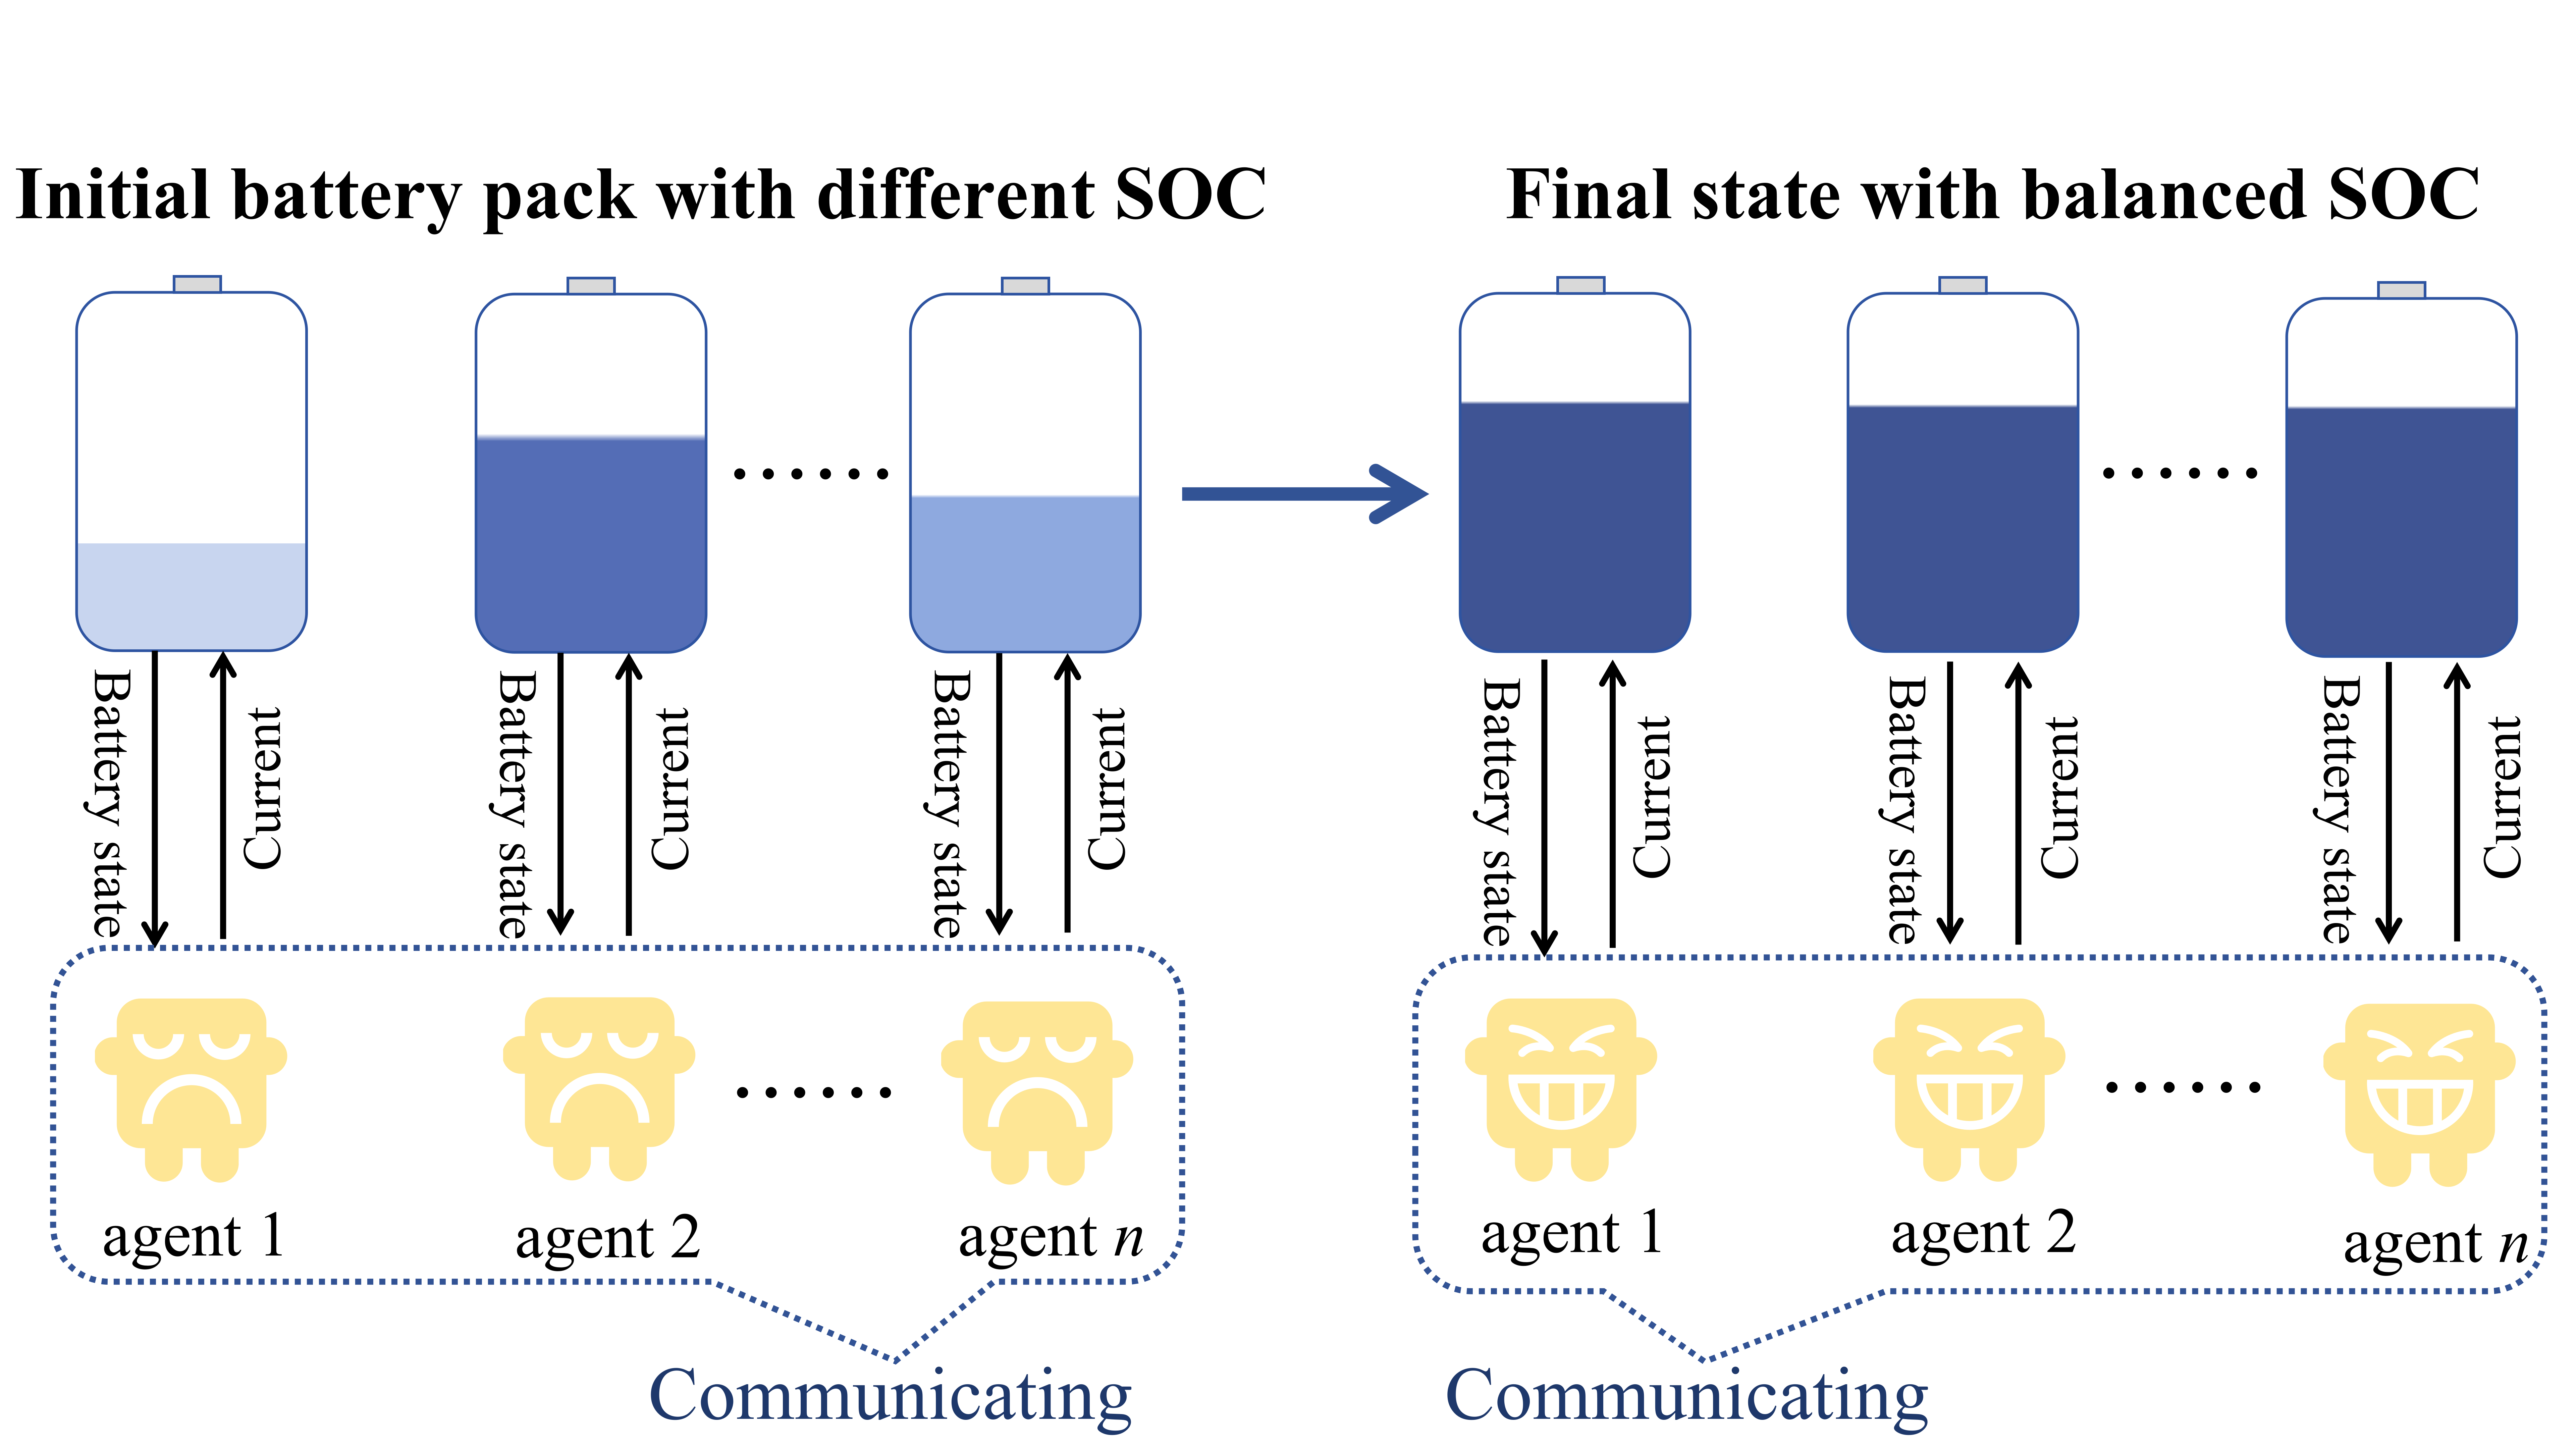
\includegraphics[width=1\linewidth]{marl_control_framework.png}
    \caption{Schematic of using the MARL-based framework to solve the charging balancing control problem.}
     \label{fig:MARL_Schematic}
 \end{figure}

\begin{figure*}
    \centering
    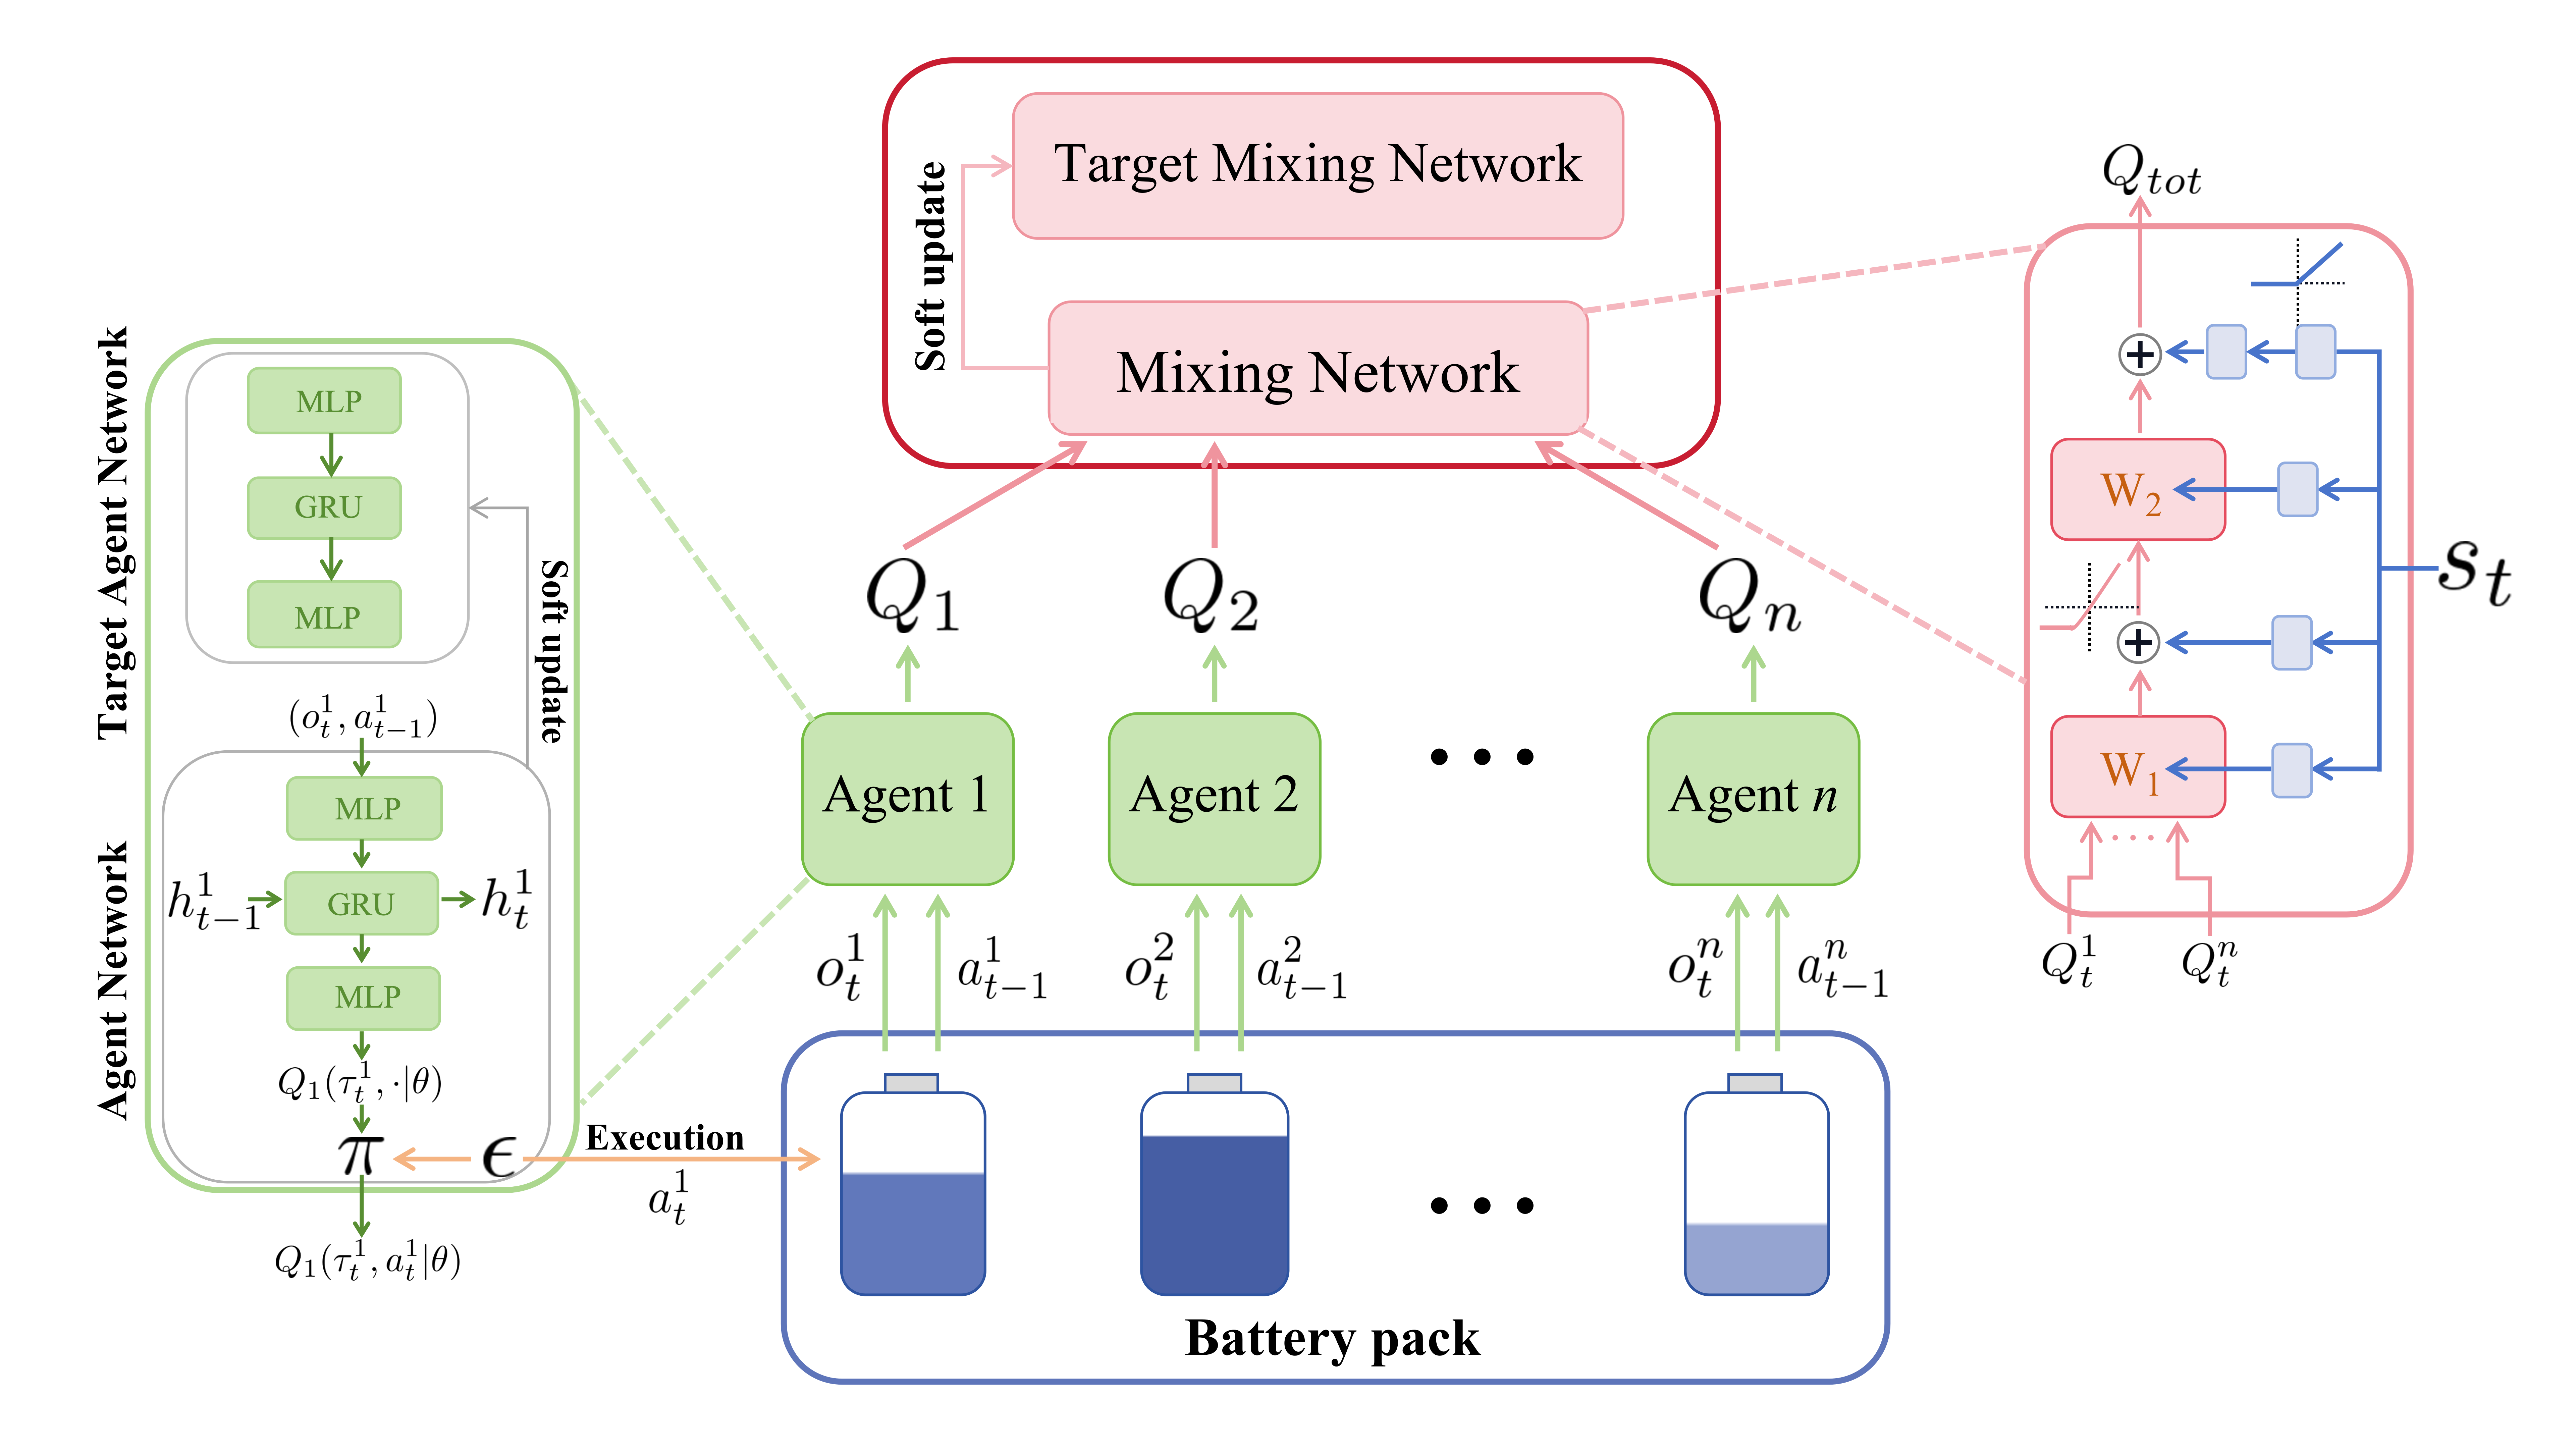
\includegraphics[width=0.9\textwidth,height=\textheight,keepaspectratio]{mba_rl_architecture.png}
    \caption{Schematic of the MBA-RL charging control framework. The left diagram depicts an agent network structure, which includes two multilayer perceptrons (MLP) and a gated recurrent unit (GRU). $\theta$ represents the parameters of the agent network. \newrev{The right diagram illustrates the mixing network, where the hypernetworks (in blue) generate the weights and biases for its layers (shown in red), and $W_1$ and $W_2$ represent the two MLP layers.}}
    \label{fig:schematic_method}
\end{figure*}

\section{\scalebox{0.84}[1]{Proposed MBA-RL for Charging Balancing Control}}
\newrev{As shown in Fig.~\ref{fig:MARL_Schematic}, each cell has a local state and an independently regulated charging current, while all cells share the objective of fast charging and pack-level SOC balancing. The resulting cooperative task uses a discrete current set and requires decentralized decisions during execution. QMIX is therefore adopted because its centralized mixing network learns a joint action value during training, while the monotonic value decomposition preserves decentralized greedy action selection \cite{26}. The QMIX controller is integrated with multiple SPMe-based cell models to form the MBA-RL framework described below.}


\subsection{MBA-RL Charging Control Framework}
\newrev{The schematic of MBA-RL is presented in Fig.~\ref{fig:schematic_method}. MBA-RL comprises shared agent networks, a mixing network, and hypernetworks. For the $i$-th agent, a recurrent Q-network combines the current observation $o_t^i$ with the previous executed action $\tilde{a}_{t-1}^i$ to form the action-observation history $\tau_t^i$ and generate the local action value $Q_i$. The mixing network combines $Q_1,Q_2,\ldots,Q_n$ into the joint action value $Q_{\mathrm{tot}}$, and the hypernetworks generate its state-dependent weights. Target agent and mixing networks provide temporal-difference targets during training. The shared agent network receives the local voltage, temperature, and SOC together with the previous-action encoding and an agent identifier.}

\newrev{We formulate the charging balancing problem as a Dec-POMDP \cite{27} described by the tuple}
{\color{red}
\begin{equation*}
\begin{aligned}
G=\langle &\mathcal{N},\mathcal{S},\{\mathcal{A}_i\}_{i=1}^{n},\mathcal{P},\mathcal{R},\\[-2pt]
&\{\mathcal{O}_i\}_{i=1}^{n},\mathcal{O},\gamma\rangle .
\end{aligned}
\end{equation*}
}
\newrev{Here, $\mathcal{N}=\{1,\ldots,n\}$ is the agent set, $\mathcal{S}$ is the global state space, $\mathcal{A}_i$ and $\mathcal{O}_i$ are the action and observation spaces of agent $i$, $\mathcal{P}$ is the transition kernel, $\mathcal{R}$ is the shared reward function, $\mathcal{O}$ is the observation function, and $\gamma$ is the discount factor.}

\subsubsection{\newrev{State and Observation Spaces}} \newrev{The global state $\mathbf{s}_t\in\mathcal{S}$ is formed by the observations of all agents at time step $t$:}
\begin{equation}
   \mathbf{s}_t = \left[ o_t^1, o_t^2, \dots, o_t^n \right]^{\mathrm{T}}
\end{equation}
\newrev{For agent $i$, the local observation $o_t^i\in\mathcal{O}_i$ consists of the cell voltage $V_i(t)$, average temperature $T_i(t)$, and $SOC_i(t)$. The observation function $\mathcal{O}$ maps the battery-pack state and joint action to the local observations available to the agents.}

\subsubsection{Action Space} \newrev{Each agent selects a requested current from the discrete candidate set $\mathcal{A}_{\mathrm{cand}}=\{0,0.5,\ldots,7.5\}\,\mathrm{A}$. Before action selection, a state-dependent availability mask removes commands that conflict with the current sampled state. Only zero current is available when $SOC_i\geq0.95$, while currents above 1 A are excluded when $V_i\geq V_{\max}$ or $T_i\geq T_{\max}$. The mask restricts the actions considered by the policy but does not predict constraint satisfaction over the next interval; therefore, the selected action is subsequently processed by the safety-constrained execution mechanism.}
\begingroup
\setlength{\abovedisplayskip}{3pt}
\setlength{\belowdisplayskip}{3pt}
\begin{equation}
\newrev{\resizebox{0.91\columnwidth}{!}{$\displaystyle
\mathbf{a}_t=\left[a_t^1,a_t^2,\dots,a_t^n\right]^{\mathrm{T}},\quad
\mathcal{A}(\mathbf{s}_t)=\prod_{i=1}^{n}\mathcal{A}_i(\mathbf{s}_t),\quad
\mathcal{A}_i(\mathbf{s}_t)\subseteq\mathcal{A}_{\mathrm{cand}}.$}}
\end{equation}
\endgroup
\subsubsection{Reward Function} \newrev{The reward combines charging progress, pack-level SOC balance, and voltage and temperature penalties:}
\begin{equation}
    r_t = r_{\text{time}} + r_{\text{bal}} + r_{\text{safety}}
\end{equation}
\newrev{The time penalty is $r_{\text{time}}=-\lambda_{\text{time}}$ before the terminal condition is reached.}

Then $r_{\text{bal}}$ can be calculated as follows:
\begin{equation}
  r_{\text{bal}} = 
\begin{cases}
 -\lambda_{\text{bal}}(\sigma - \beta), & \text{if } \sigma \geq \beta \\
0, & \text{otherwise}
\end{cases}  
\end{equation}
where $\sigma$ denotes the standard deviation of the SOC across all cells in the battery pack, $\beta$ indicates the predefined threshold, and $r_{\text{bal}}$ characterizes the imbalance effects in the battery pack. 

As shown in \eqref{safty condition}, $r_{\text{safety}}$ is divided into voltage safety constraints and temperature safety constraints:
\begin{equation}
    r_{\text{safety}} = r_{\text{volt}} + r_{\text{temp}}
\end{equation}
\begin{equation}
    \quad r_{\text{volt}} = \sum_{i=1}^{n} \delta_{v,i}, \quad r_{\text{temp}} = \sum_{i=1}^{n} \delta_{t,i}
\end{equation}
where $\delta_{v,i}$ and $\delta_{t,i}$ represent the overvoltage and overtemperature penalties of the $i$-th cell, respectively:
\begin{equation}
    \delta_{v,i} = 
\begin{cases}
 -\lambda_v(V_i(t) - V_{\text{max}}), & \text{if } V_i(t) \geq V_{\text{max}} \\
0, & \text{otherwise}
\end{cases}
\end{equation}

\begin{equation}
  \delta_{t,i} = 
\begin{cases}
 -\lambda_T(T_i(t) - T_{\text{max}}), & \text{if } T_i(t) \geq T_{\text{max}} \\
0, & \text{otherwise}
\end{cases}  .
\end{equation}
\subsubsection{\newrev{Transition and Termination}} \newrev{The safety screen is treated as part of the action-execution interface. Given the requested joint action $\mathbf{a}_t$, it produces the executed action $\tilde{\mathbf{a}}_t$, and the transition kernel $\mathcal{P}(\mathbf{s}_{t+1}\mid\mathbf{s}_t,\mathbf{a}_t)$ is induced by this screening operation and the battery dynamics. The variable $done$ is defined separately as the episode-termination indicator.}

\begin{algorithm}[t]
    \caption{MBA-RL charging control framework}
    \label{alg:QMIX}
    
    \begin{algorithmic}[1]
        \STATE Initialize $\theta, \theta', \bm{\theta}, \bm{\theta}'$ randomly
        \STATE Set the learning rate $\alpha$, number of episodes $N_{episode}$, and replay buffer $\mathcal{D}$
        \STATE $\theta' \leftarrow \theta, \bm{\theta}' \leftarrow \bm{\theta}$
        \FOR{$episode =$ 1 to $N_{episode}$}
            \STATE $t\leftarrow 0$, $\tau_t^i \leftarrow \emptyset$, and observe the initial state $\mathbf{s}_t$

            // \textbf{Data Collection}
            \WHILE{$\neg done$}
                \FOR{the $i$-th agent}
                    \STATE \newrev{$\tau_t^i \leftarrow \tau_{t-1}^i \cup \{(o_t^i, \tilde{a}_{t-1}^i)\}$}
                    \STATE \newrev{Update $\epsilon$ according to the exploration schedule}
                    \STATE Select the requested action $a_t^i$ according to \eqref{epsilon-greedy}
                \ENDFOR
                \STATE \newrev{Screen $\mathbf{a}_t$ to obtain $\tilde{\mathbf{a}}_t$, execute $\tilde{\mathbf{a}}_t$, observe $r_t$, and get $\mathbf{s}_{t+1}$}
                \STATE \newrev{$\mathcal{D} \leftarrow \mathcal{D} \cup \{ \langle\mathbf{s}_t, \mathbf{m}_t, \mathbf{a}_t, \tilde{\mathbf{a}}_t, r_t, \mathbf{s}_{t+1}, \mathbf{m}_{t+1}, done\rangle \}$}
            \ENDWHILE
            
            // \textbf{Network Update}
            \IF{$|\mathcal{D}| > N$}
                \STATE $B \leftarrow$ Randomly sample data from $N$ episodes in $\mathcal{D}$
                \FOR{each time step $t$ in each episode in batch $B$}
                    \STATE Calculate $Q_{tot}$ by \eqref{Q-value} based on the state $\mathbf{s}_t$
                    \STATE Calculate $y^{\text{tot}}$ by \eqref{target Q} based on the state $\mathbf{s}_{t+1}$
                \ENDFOR
                \STATE Under the conditions given in \eqref{QMIX_constraints} and \eqref{QMIX_constraints_1}, utilize the RMSprop  optimizer \cite{zou2019sufficient} to update $\theta$ and $\bm{\theta}$ by minimizing the loss function: $\left( y_{\text{tot}} - Q_{\text{tot}} \right)^2$
            \ENDIF
            \IF{$episode$ \% $N_t$ == 0}
                \STATE $\theta' \leftarrow \theta$, $\bm{\theta}' \leftarrow \bm{\theta}$ 
            \ENDIF
        \ENDFOR
    \end{algorithmic}
\end{algorithm}

\subsection{Safety-Constrained Execution}
\newrev{At each decision step, MBA-RL generates a requested current for every cell. Starting from this request, the safety screen evaluates successively lower candidate currents with the nominal SPMe over the next decision interval and a subsequent zero-current interval. Prediction corrections derived from the observed-model mismatch are added to the predicted SOC, voltage, and temperature peaks. The largest candidate satisfying the margins specified in Table~\ref{tab:experimental_settings} is executed. If no feasible candidate exists for any cell, the episode terminates without advancing the battery model. The same screen is used during training and execution. It provides a sampled finite-horizon check rather than a continuous-time safety guarantee.}

\subsection{Balancing Mechanism of MBA-RL}

\begin{figure}[t]
    \centering
    \includegraphics[width=0.95\linewidth]{experimental_platform.png}
    \caption{Schematic of the experimental platform.}
    \label{fig:experiment_Schematic}
\end{figure}

\newrev{MBA-RL uses global information during centralized training so that each agent accounts for the charging-time objective in \eqref{eqn:balancing objective} together with the pack-level balancing requirement in \eqref{terminal balance}.}

In MBA-RL, the $i$-th agent aims to optimize its local Q-value, denoted as $Q_i(\tau_t^i, a_t^i|\theta)$, to maximize the global Q-value $Q_{\text{tot}}$. This involves balancing the agent's own goals of safety and fast charging while simultaneously contributing to the rapid achievement of balance within the battery pack. Each agent chooses its current action $a_t^i$ using the $\epsilon$-greedy strategy, which can be described as follows:
\begin{equation}\label{epsilon-greedy}
a_t^i =
\begin{cases}
\text{random available action} & \text{with probability } \epsilon \\
\arg\max_{a_t^i} Q_i(\tau_t^i, a_t^i|\theta) & \text{with probability } 1 - \epsilon
\end{cases}
\end{equation}
where $Q_i(\tau_t^i, a_t^i|\theta)$ is computed based on $\tau_t^i$ and $a_t^i$. \rev{All agents share a common set of parameters $\theta$. A one-hot agent identifier is appended to each network input so that the shared network can represent cell-specific action values.}

\newrev{The mixing network takes the outputs of all agent networks as inputs and combines them monotonically to generate $Q_{tot}(\boldsymbol{\tau}_t, \mathbf{a}_t|\bm{\theta})$:}
\begin{equation}\label{Q-value}
    Q_{tot}(\boldsymbol{\tau}_t, \mathbf{a}_t|\bm{\theta}) = f(Q_1(\tau_t^1, a_t^1|\theta), ..., Q_n(\tau_t^n, a_t^n|\theta))
\end{equation}
where $\boldsymbol{\tau}_t$ denotes the joint action-observation history at the time step $t$, and $\bm{\theta}$ represents the parameters of the mixing network. 

The final objective of MBA-RL is to maximize the global Q-value $Q_{tot}(\boldsymbol{\tau}_t, \mathbf{a}_t|\bm{\theta})$. \newrev{The mixing network enforces a monotonicity constraint between the joint and local action values, so decentralized greedy action selection is consistent with joint greedy selection:}
\begin{equation}\label{QMIX_constraints}
\arg\max_{\mathbf{a}_t} Q_{tot}(\boldsymbol{\tau}_t, \mathbf{a}_t|\bm{\theta}) =
\begin{pmatrix}
\arg\max_{a_t^1} Q_1(\tau_t^1, a_t^1|\theta) \\
\vdots \\
\arg\max_{a_t^n} Q_n(\tau_t^n, a_t^n|\theta)
\end{pmatrix}.
\end{equation}
Eq. \eqref{QMIX_constraints} enables each agent to greedily select the action that maximizes $Q_i(\tau_t^i, a_t^i|\theta)$ for decentralized execution. 

\newrev{The hypernetworks receive the state $s_t$ and generate nonnegative weights for the mixing network, enforcing}
\begin{equation}\label{QMIX_constraints_1}
\frac{\partial Q_{tot}}{\partial Q_i} \geq 0, \, i = 1, 2, ..., n.
\end{equation}

\newrev{The target agent and mixing networks are initialized from their corresponding online networks and synchronized every $N_t$ training episodes. Considering the terminal flag and the availability mask at the next state, the global target Q-value is computed as}
\begin{equation}\label{target Q}
\newrev{y_t^{\text{tot}} = r_t + \gamma(1-d_t) \max_{\mathbf{a}_{t+1}\in\mathcal{A}(\mathbf{s}_{t+1})} Q_{\text{tot}}(\boldsymbol{\tau}_{t+1}, \mathbf{a}_{t+1}|\bm{\theta}'),}
\end{equation}
\newrev{where $d_t$ denotes the terminal flag.}

\newrev{Complete episodes are stored in the replay buffer $\mathcal{D}$ together with the observations, availability masks, requested and executed actions, rewards, and terminal flags. During training, a batch of episodes is randomly sampled for network updates. The Q-function is indexed by the requested action selected by the policy, while the executed action is included in the subsequent action-observation history to account for intervention by the safety screen.}

In summary, the details of the MBA-RL charging control framework are described in Algorithm 1, where $|\cdot|$ denotes the cardinality of a set.

\begin{figure}[t]
    \centering

    \begin{subfigure}[t]{0.24\textwidth} 
        \centering
        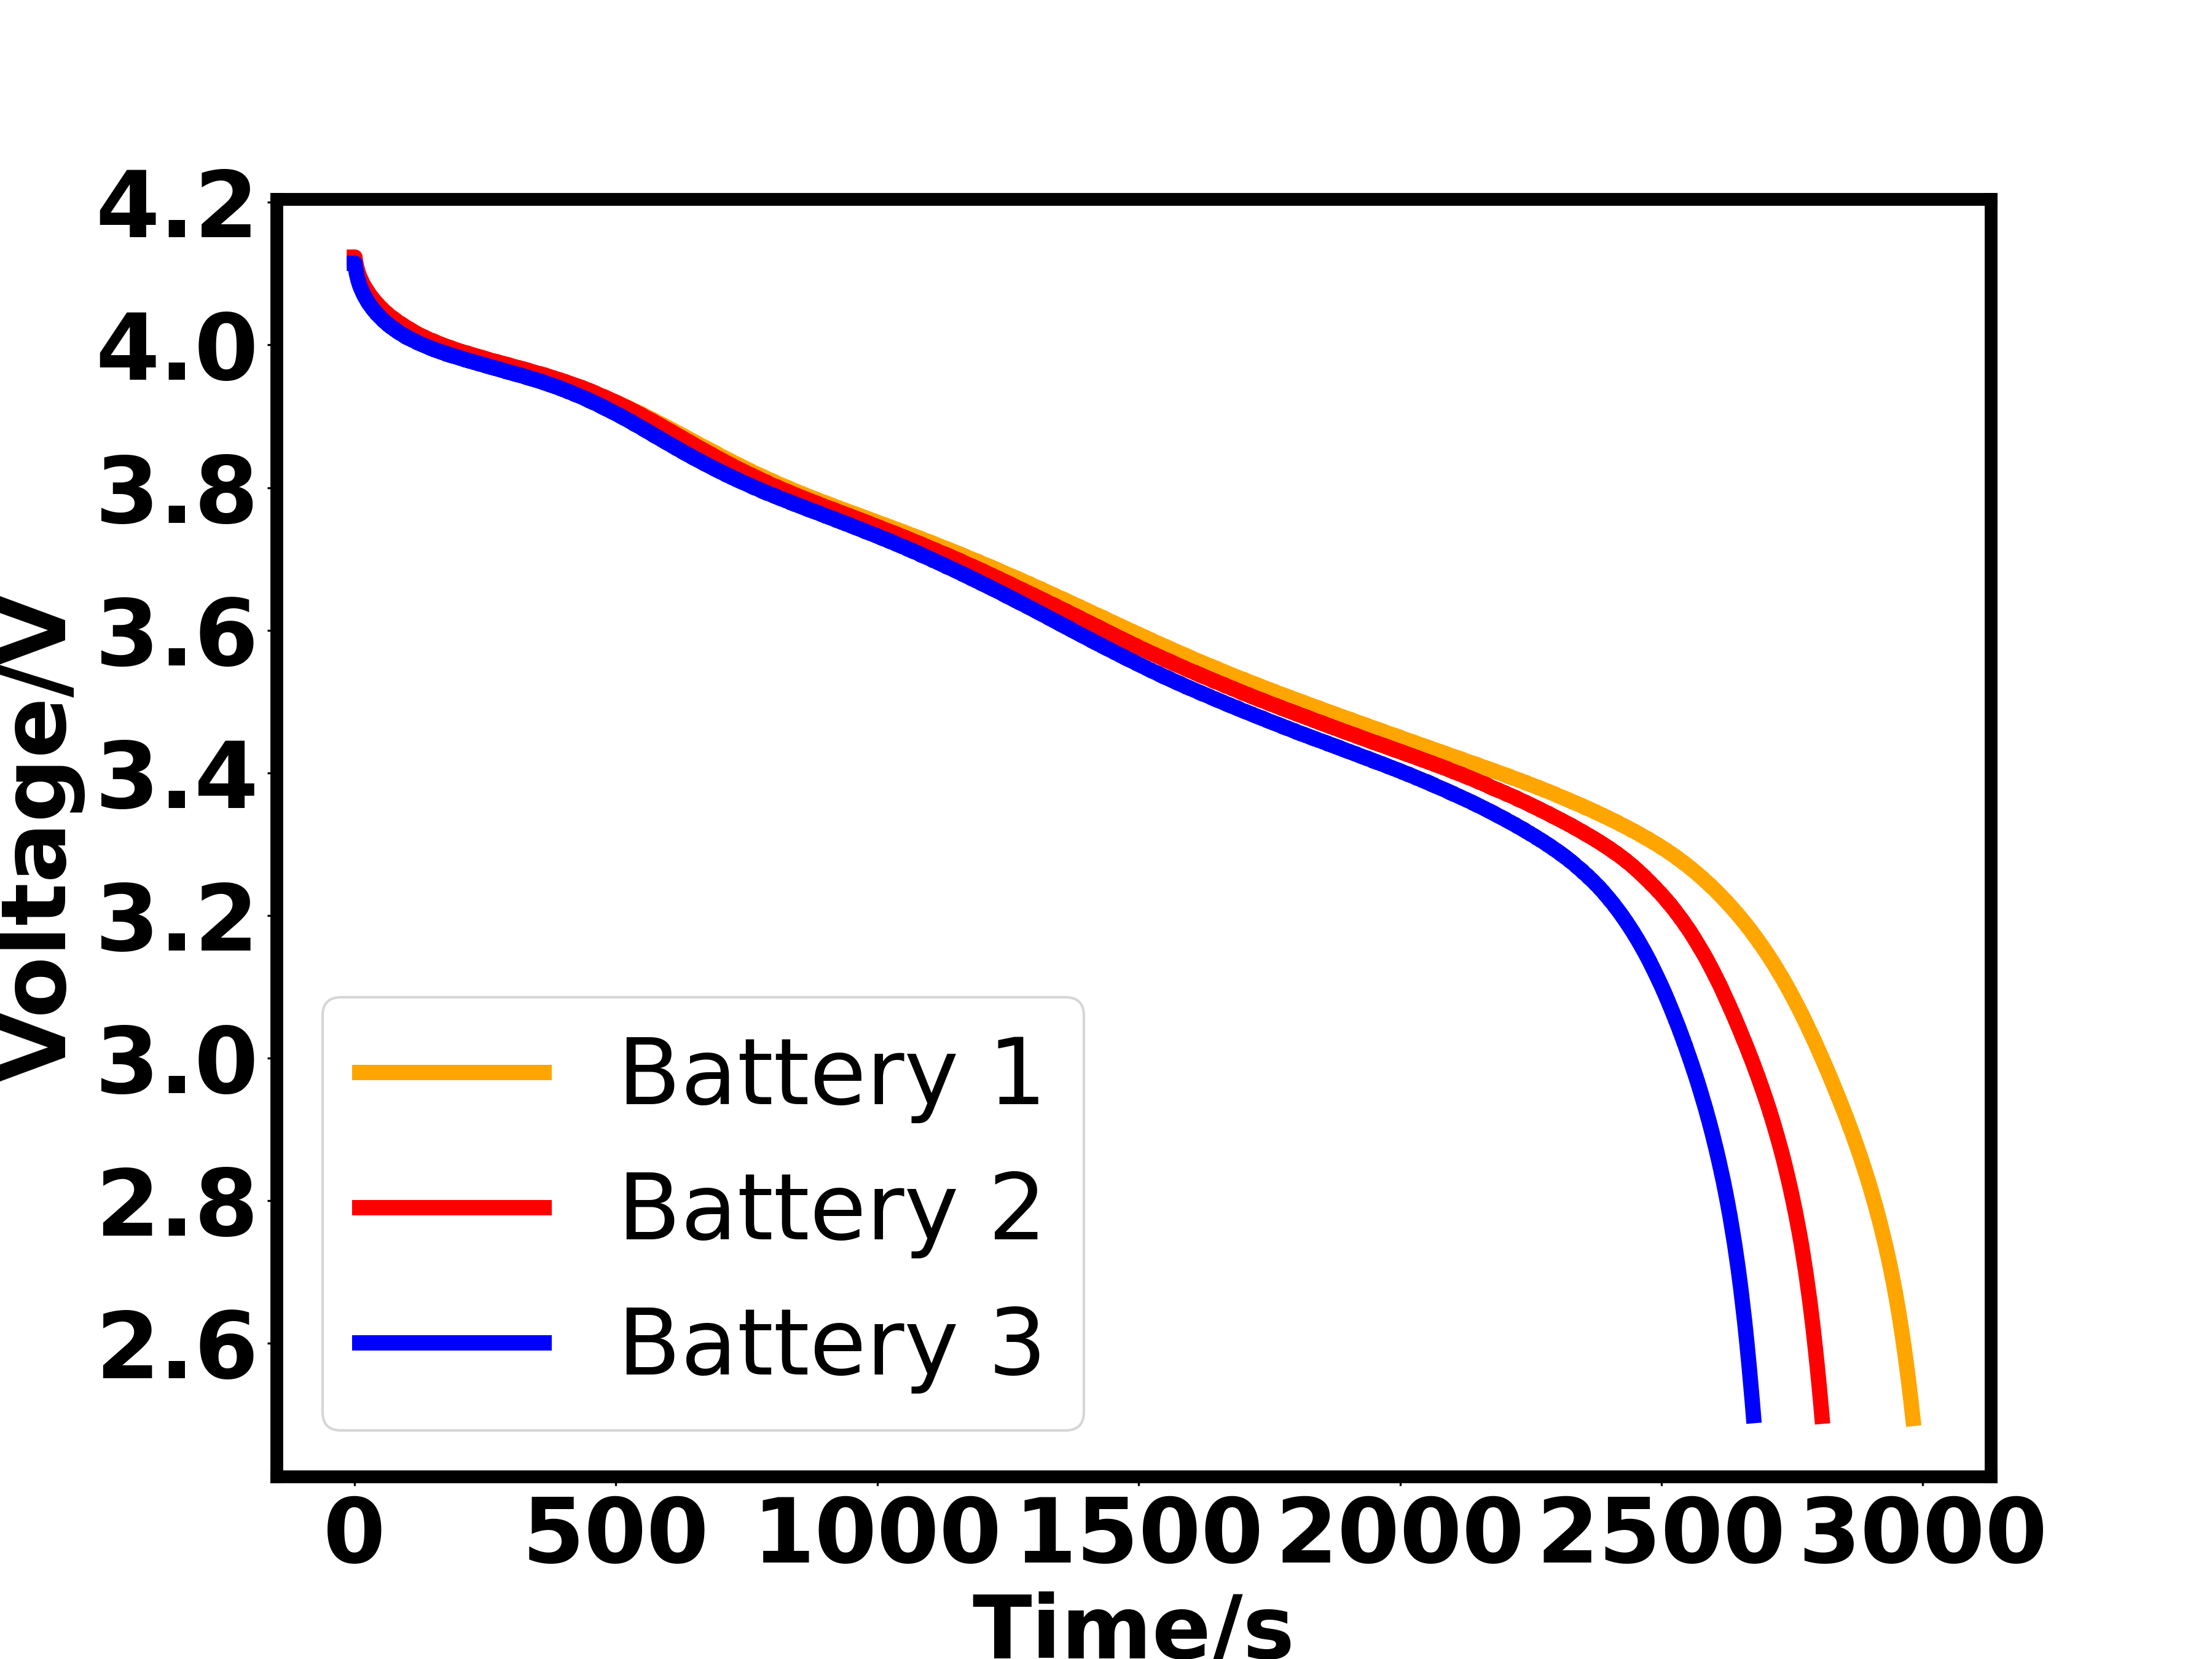
\includegraphics[width=\textwidth]{aging_voltage.png}
        \caption{}
    \end{subfigure}
    \hfill
    \begin{subfigure}[t]{0.24\textwidth}
        \centering
        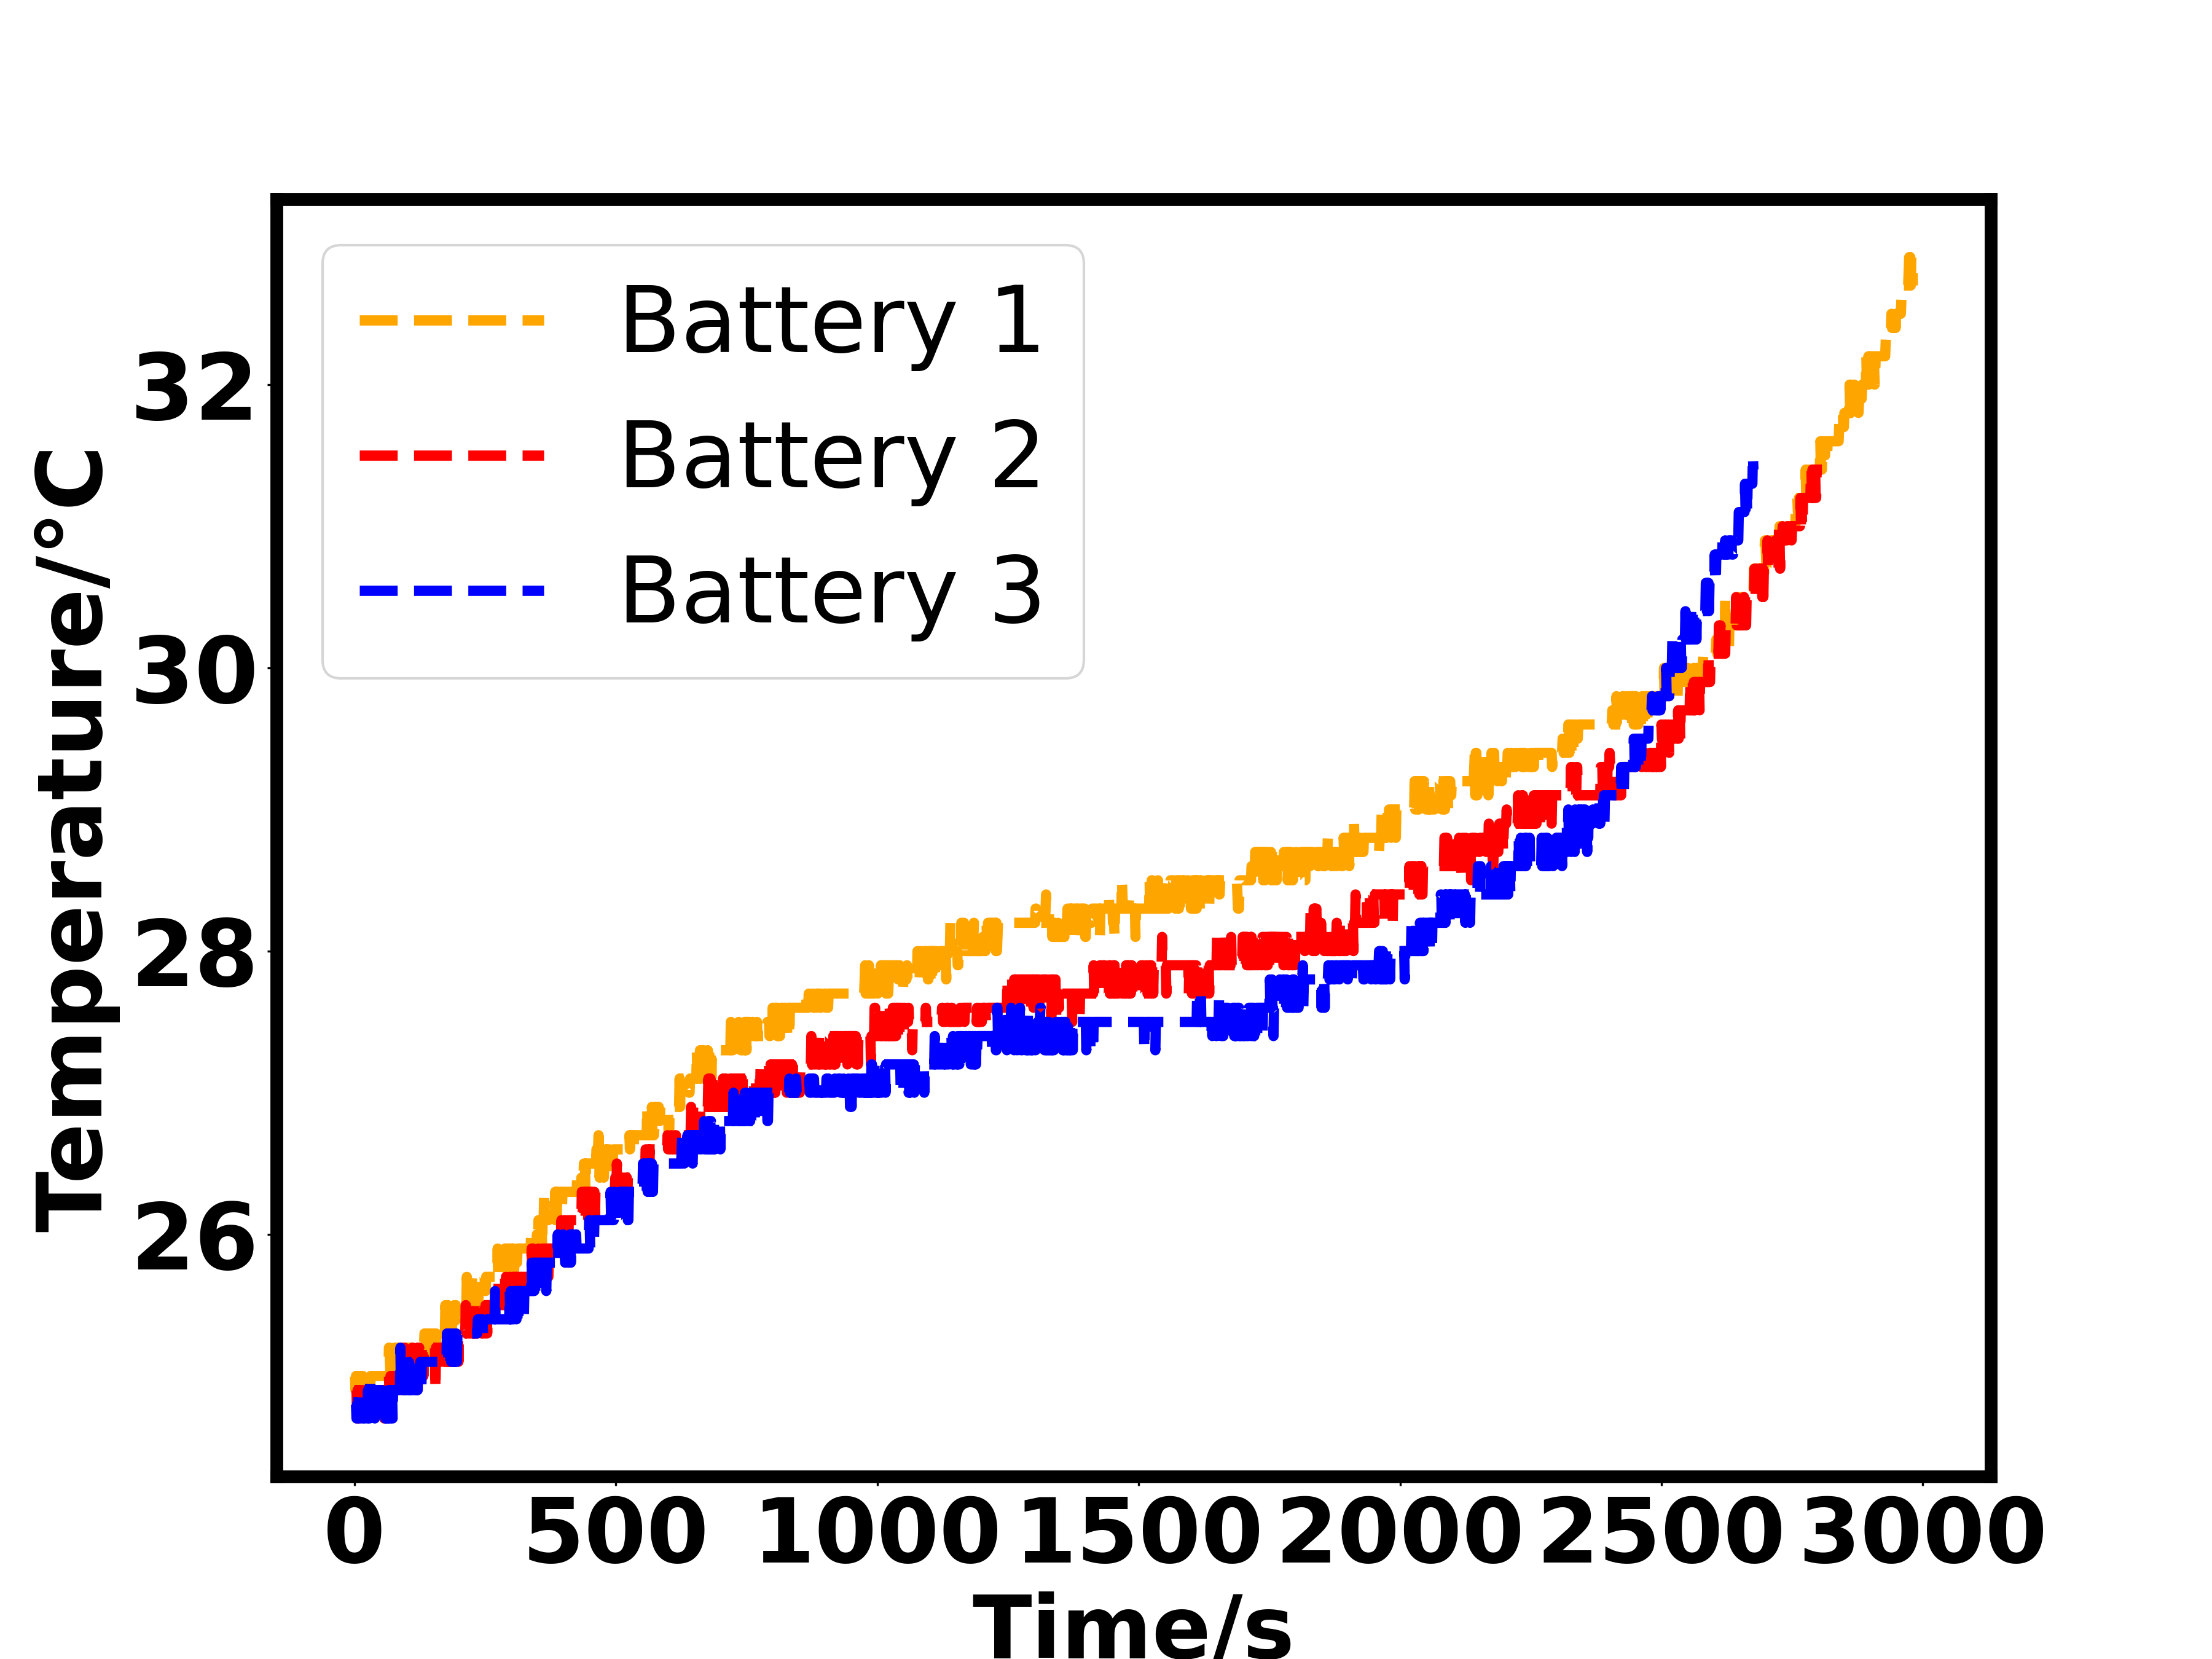
\includegraphics[width=\textwidth]{aging_temperature.png} 
        \caption{}
    \end{subfigure}

    \caption{Voltage and temperature curves of the three cells at 1 C discharging current. (a) Voltage curve. (b) Temperature curve.}
    \label{fig:three_aging}
\end{figure}

\begin{figure}[t]
    \centering

    \begin{subfigure}[t]{0.24\textwidth} 
        \centering
        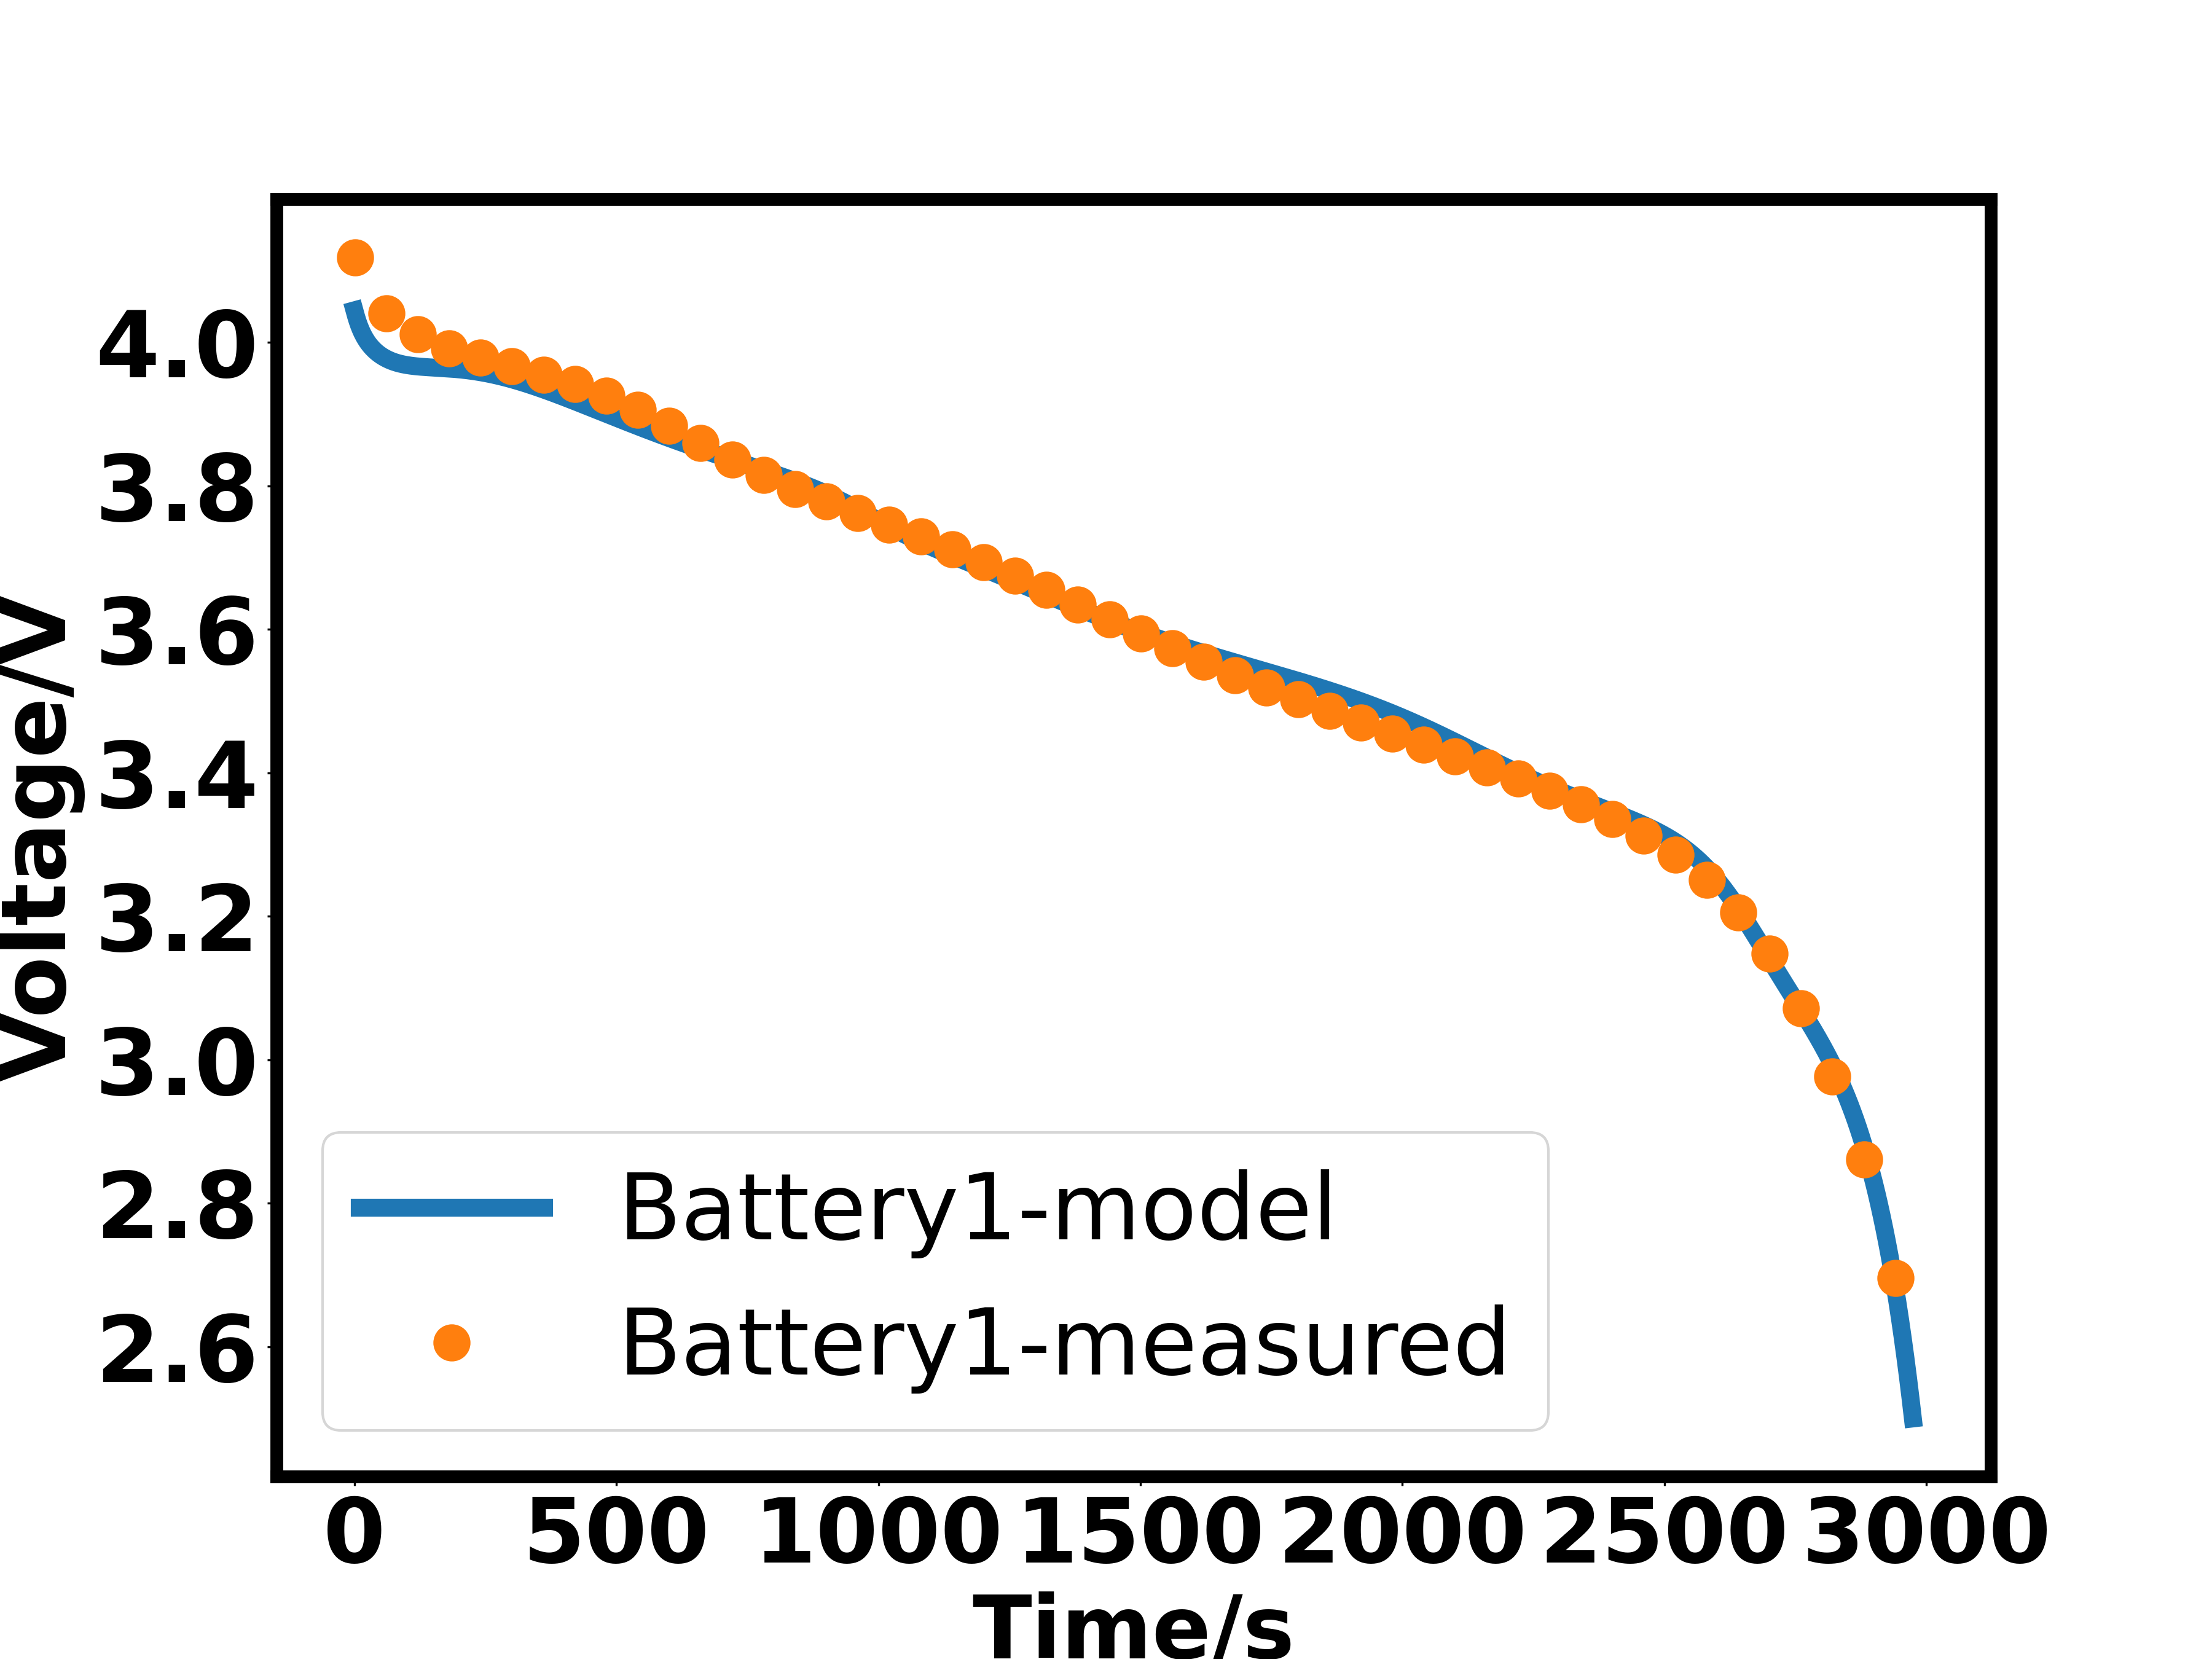
\includegraphics[width=\textwidth]{cell1_voltage_fit.png}
        \caption{}
    \end{subfigure}
    \hfill
    \begin{subfigure}[t]{0.24\textwidth}
        \centering
        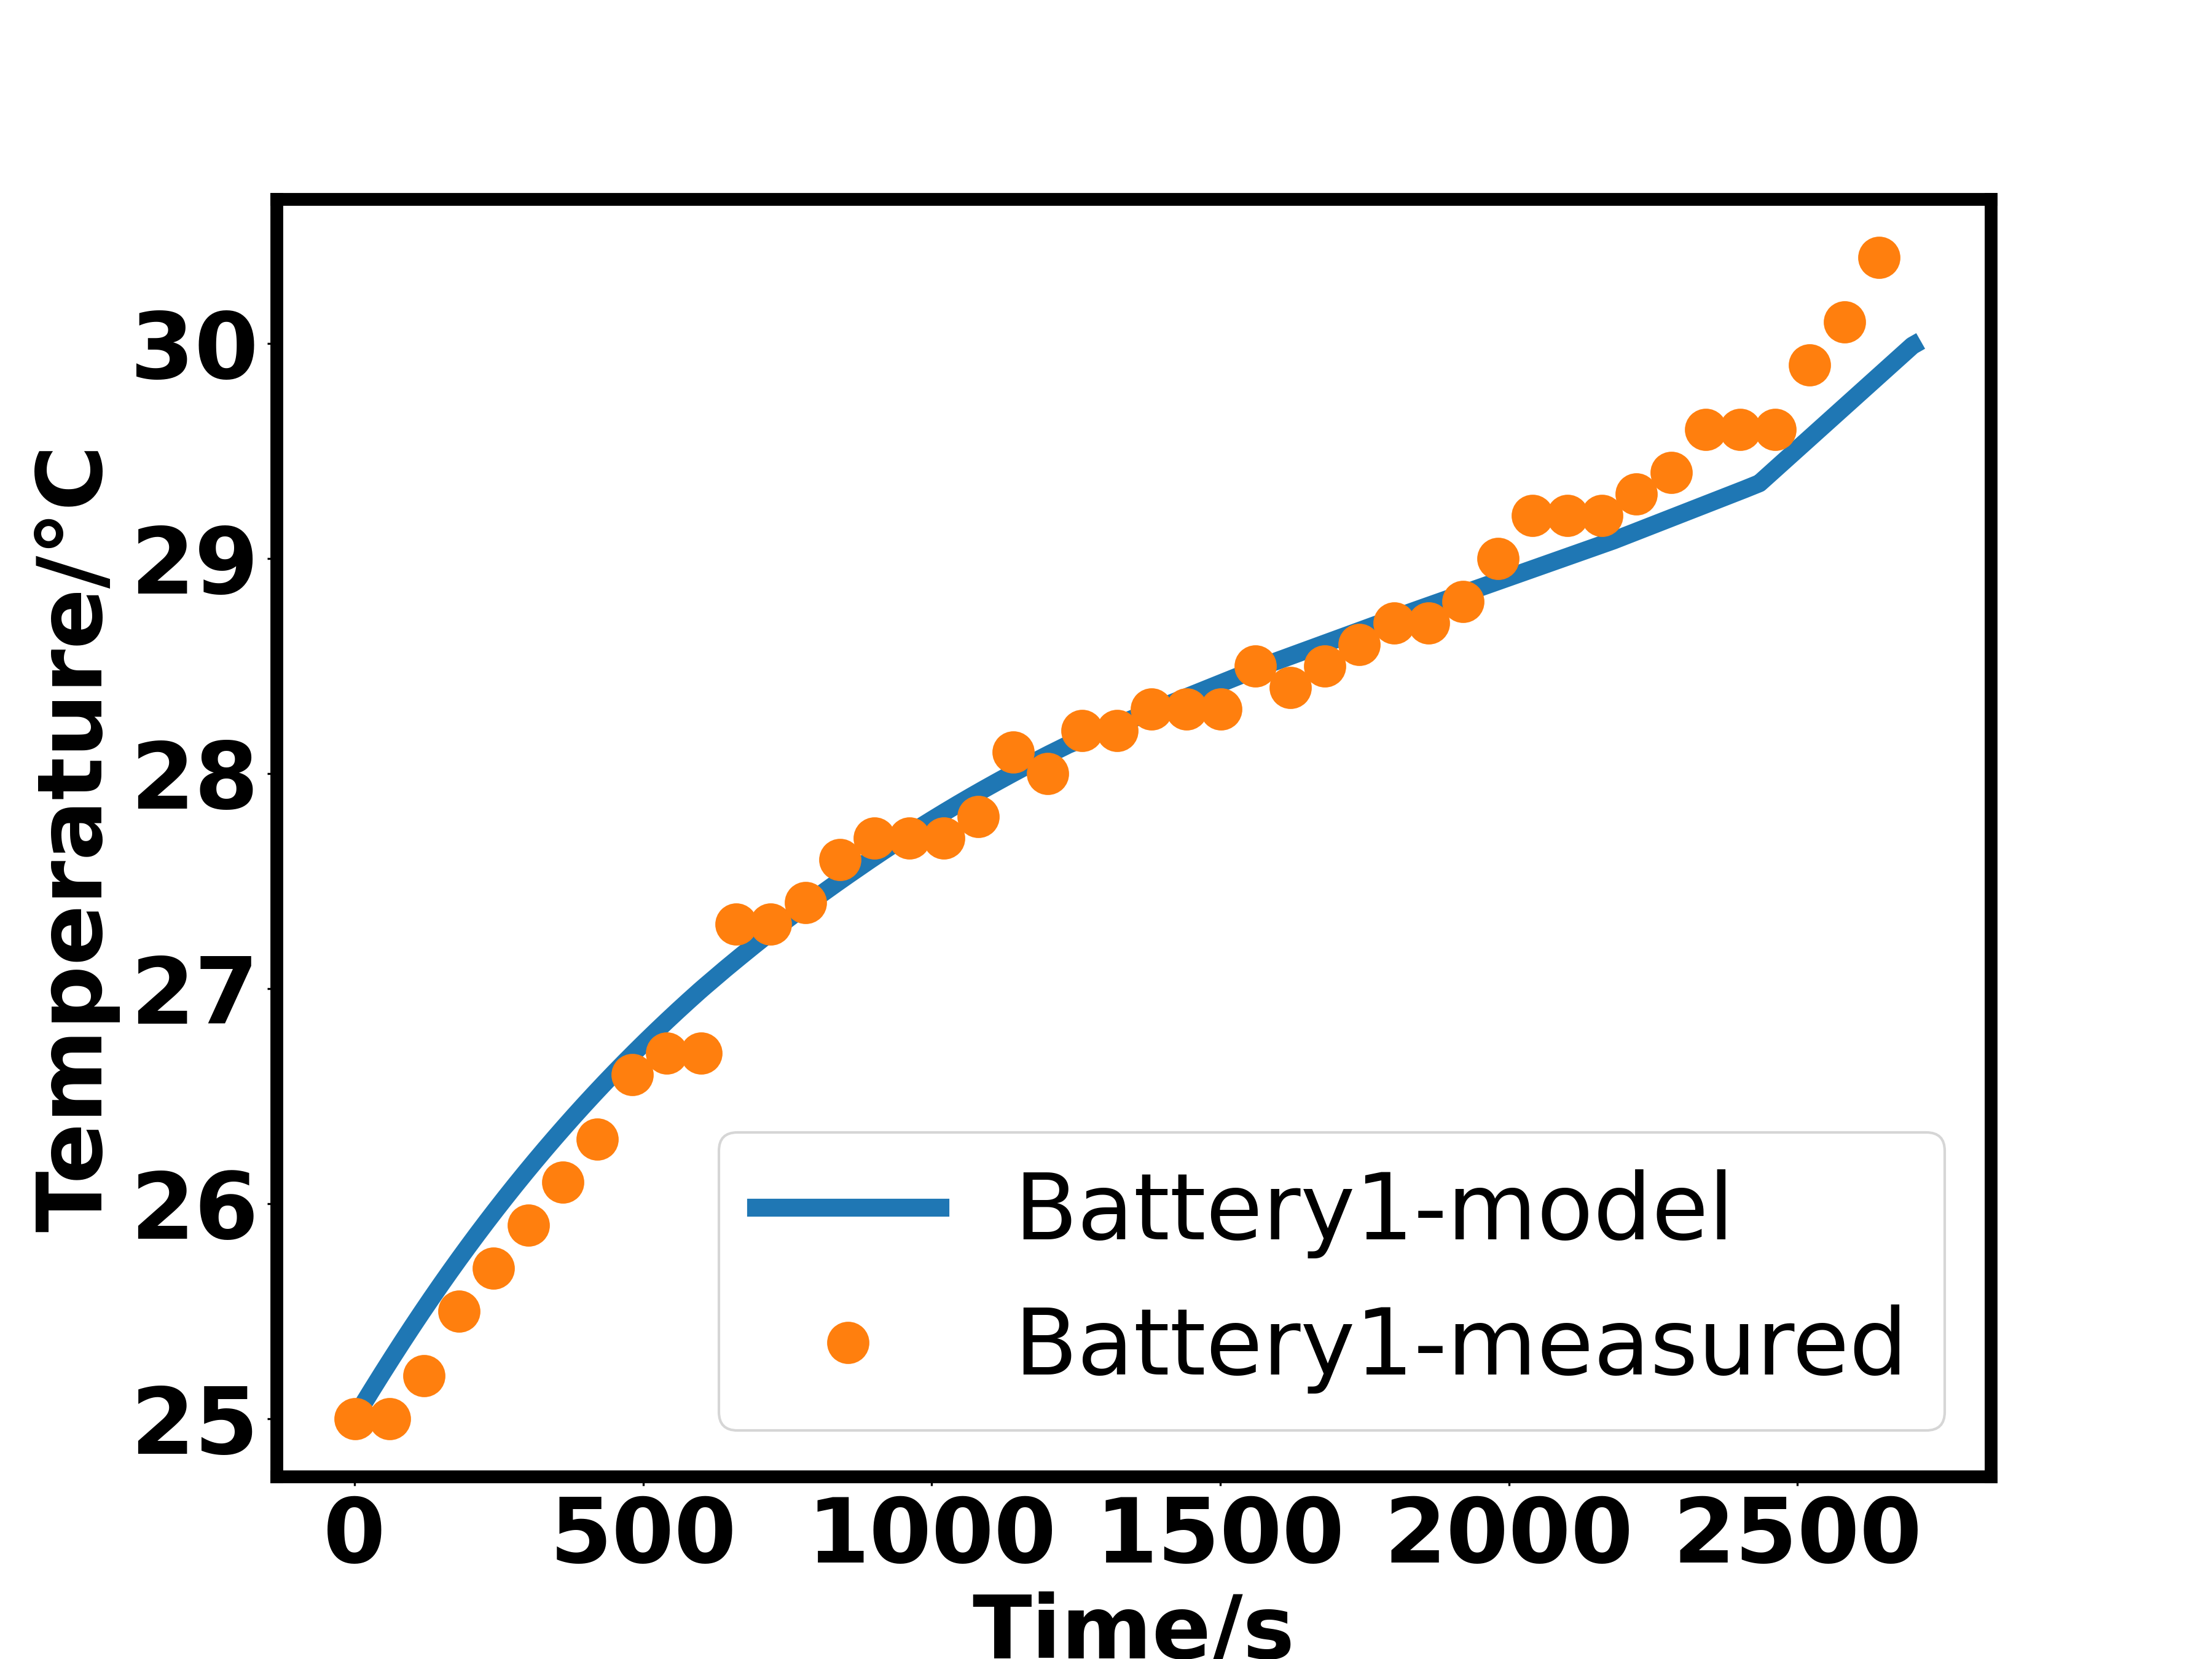
\includegraphics[width=\textwidth]{cell1_temperature_fit.png} 
        \caption{}
    \end{subfigure}

    \caption{Parameter identification results for Cell 1. (a) Electrochemical model parameter identification. (b) Thermal model parameter identification.}
    \label{battery1}
\end{figure}

\begin{figure}[t]
    \centering

    \begin{subfigure}[t]{0.24\textwidth} 
        \centering
        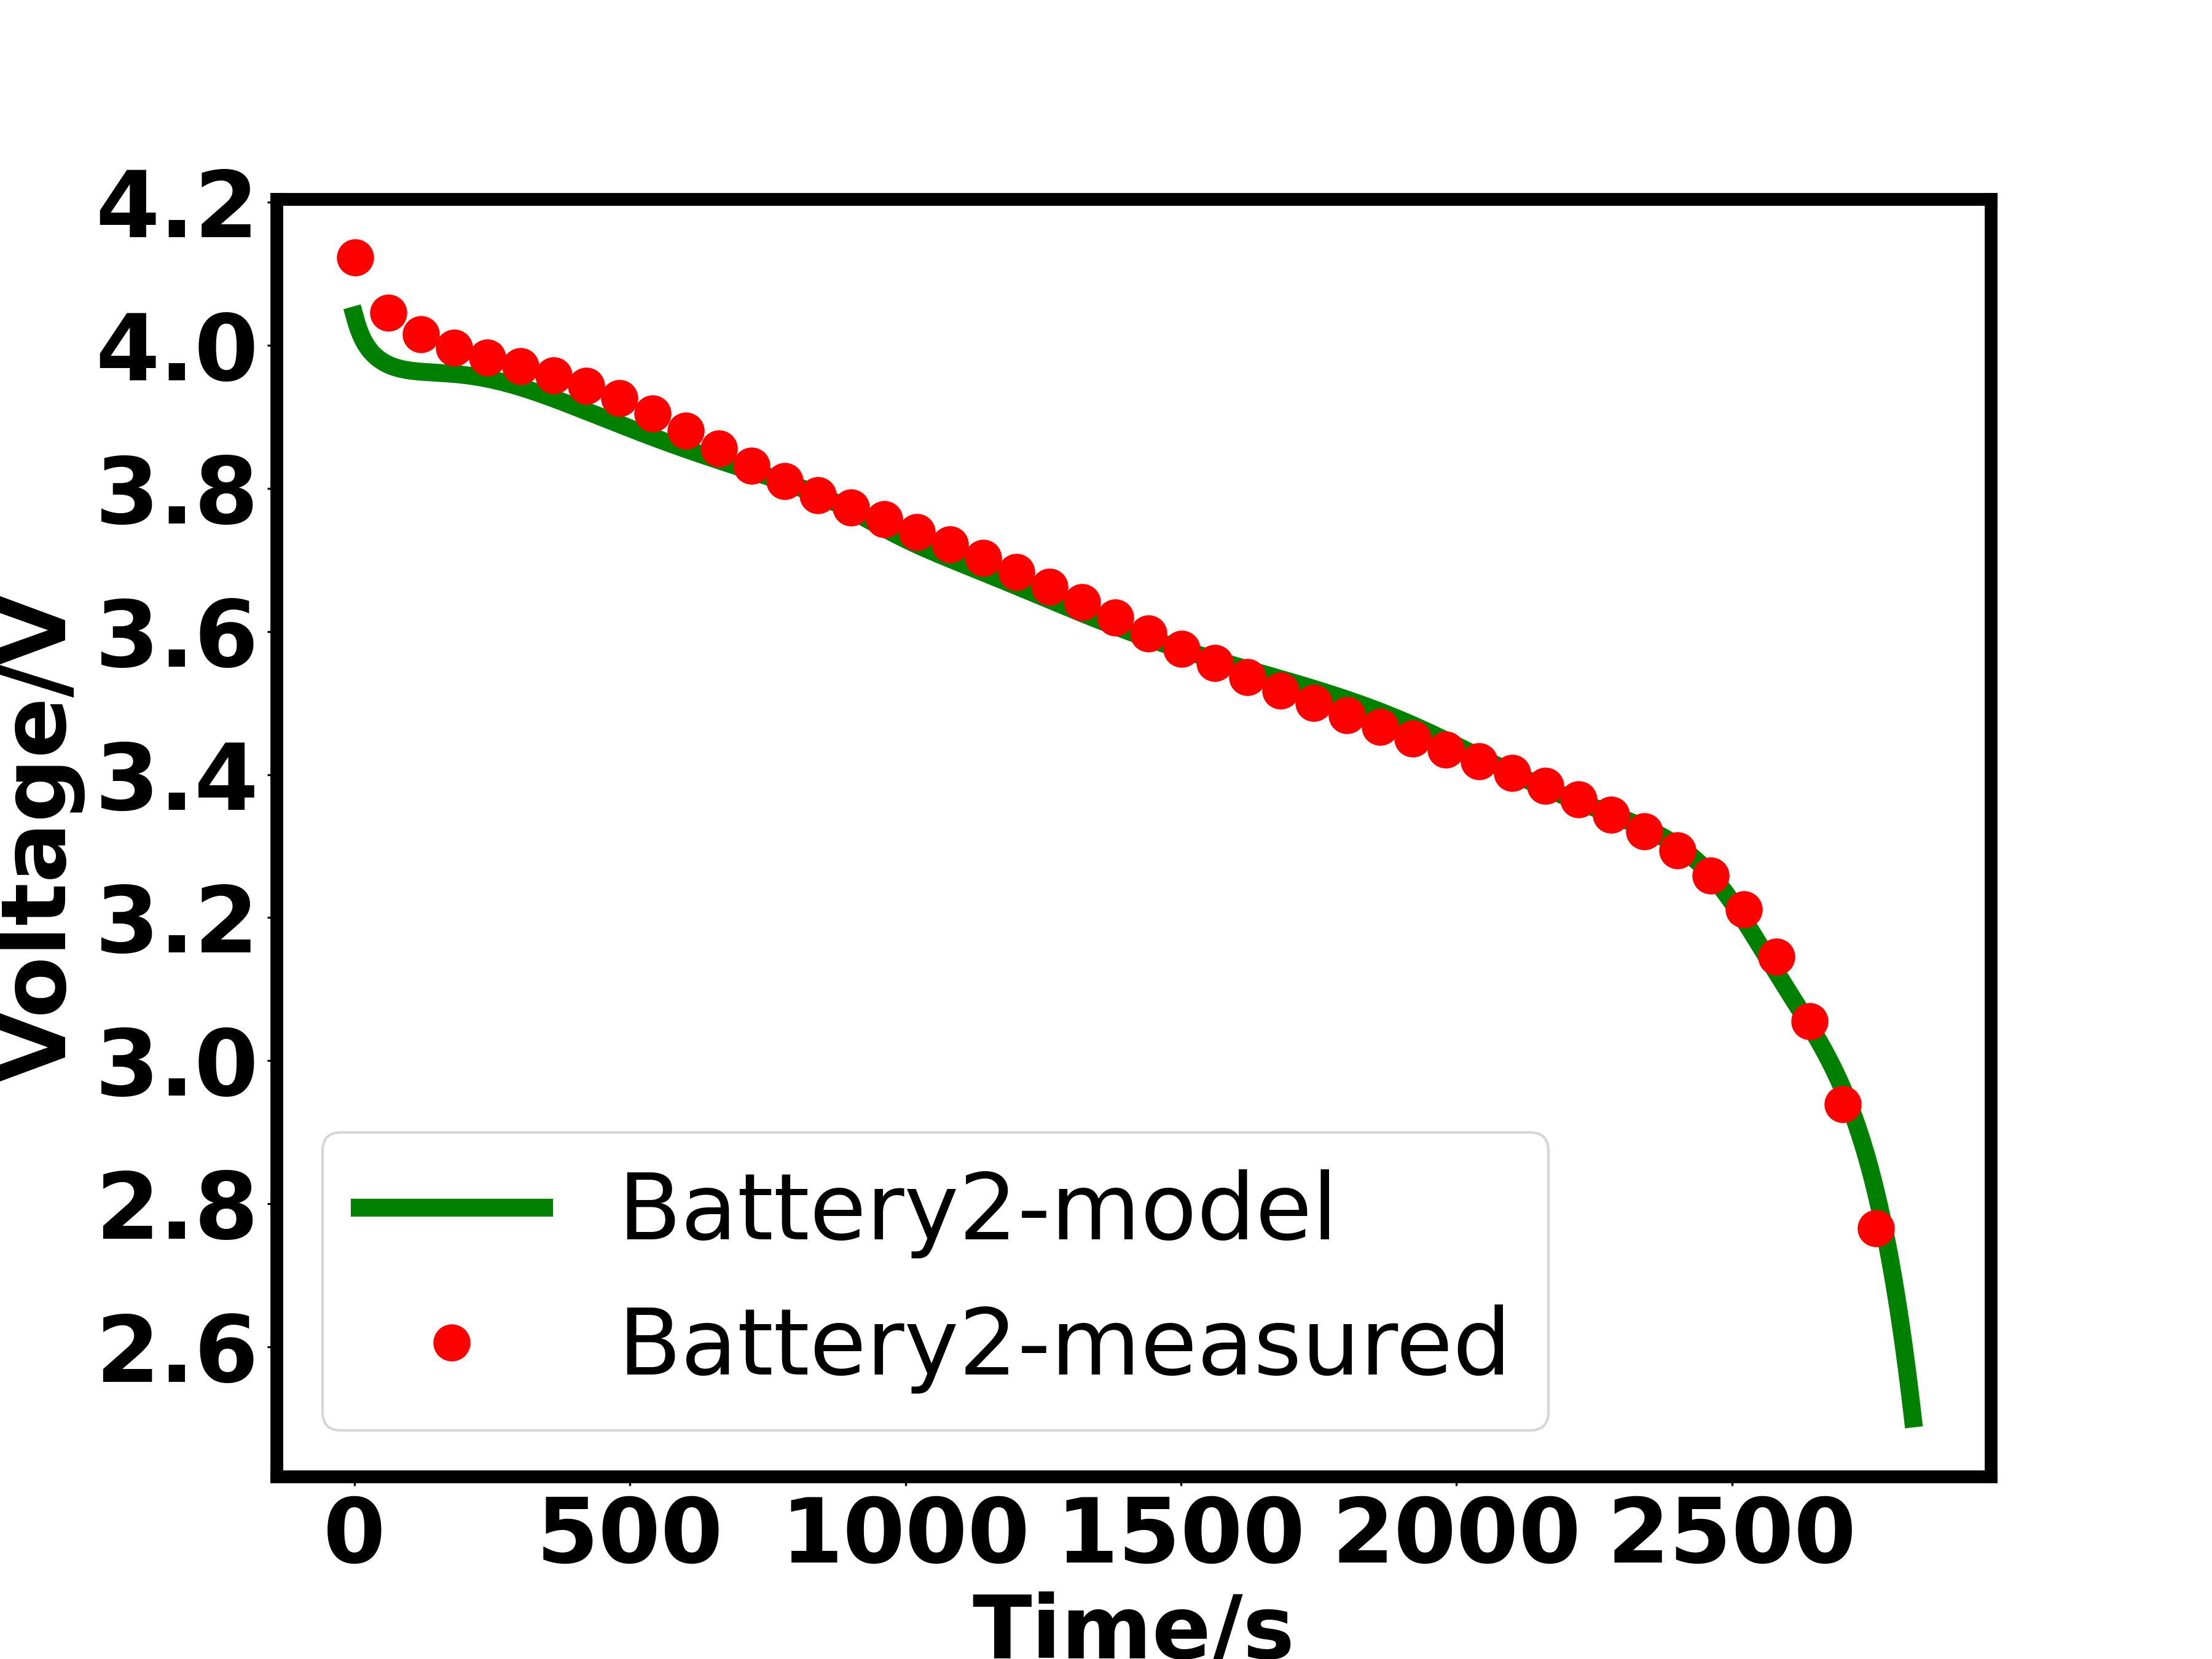
\includegraphics[width=\textwidth]{cell2_voltage_fit.png}
        \caption{}
    \end{subfigure}
    \hfill
    \begin{subfigure}[t]{0.24\textwidth}
        \centering
        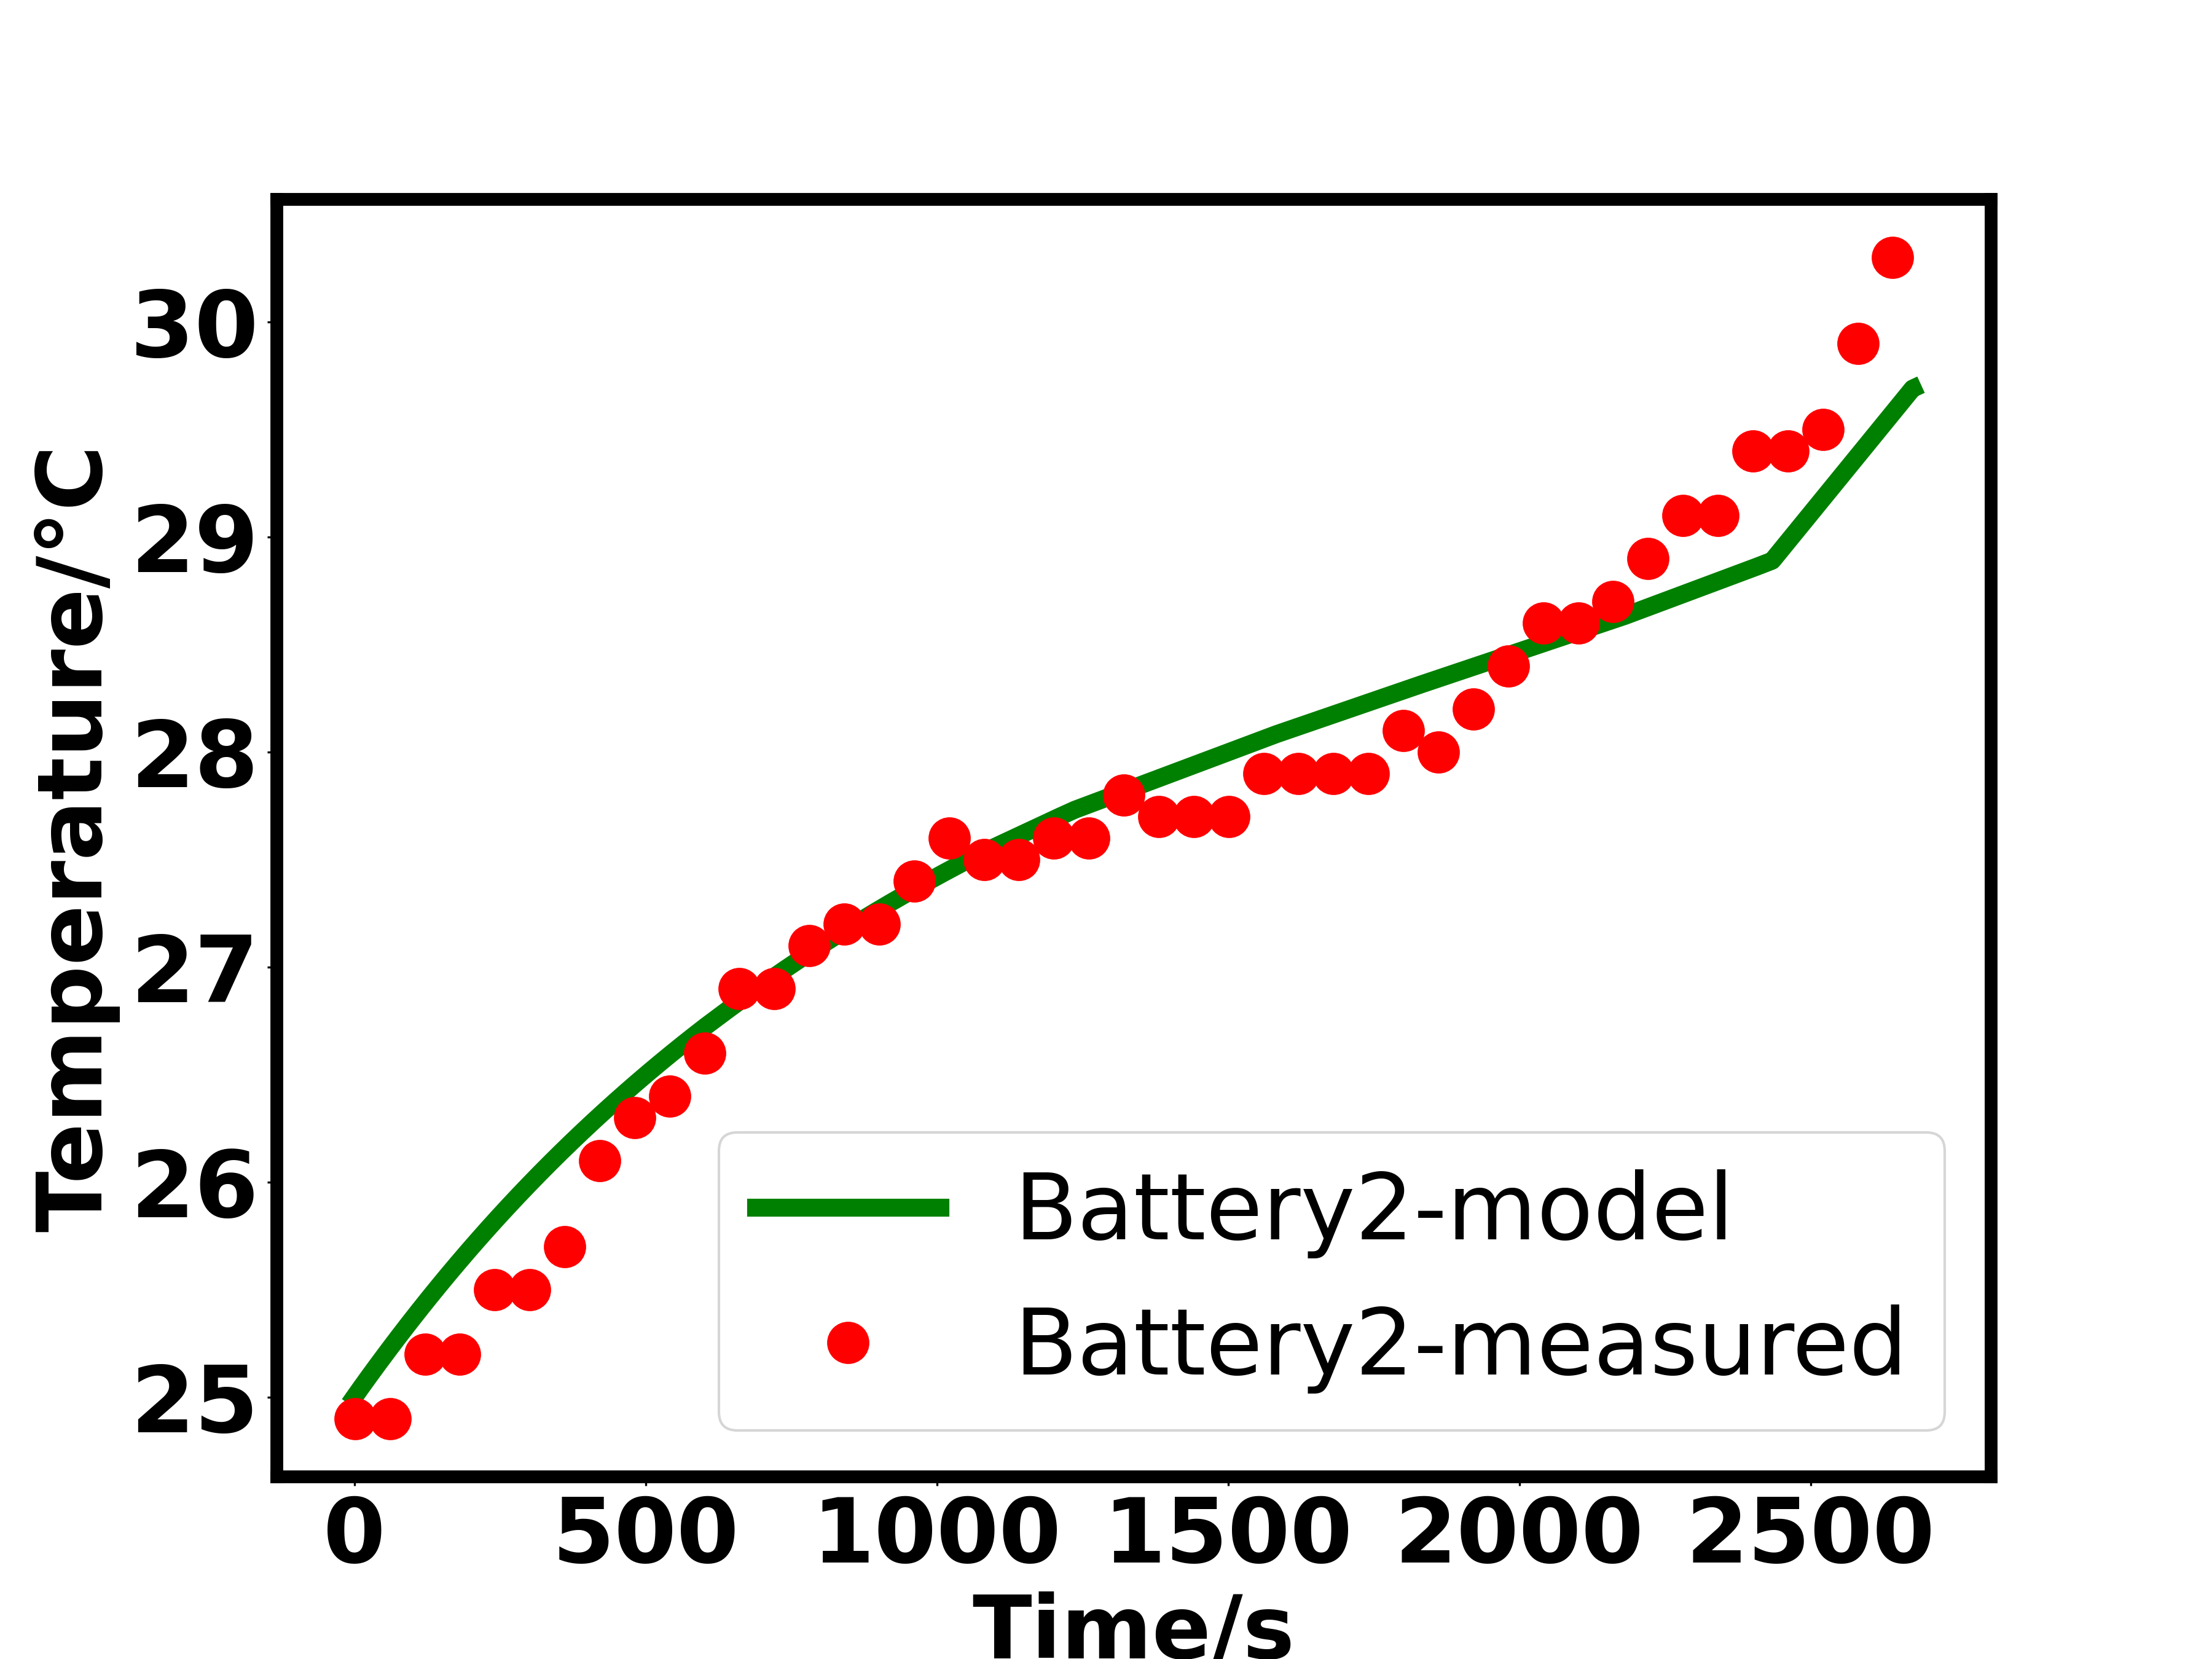
\includegraphics[width=\textwidth]{cell2_temperature_fit.png} 
        \caption{}
    \end{subfigure}

    \caption{Parameter identification results for Cell 2. (a) Electrochemical model parameter identification. (b) Thermal model parameter identification.}
    \label{battery2}
\end{figure}

\begin{figure}[t]
    \centering

    \begin{subfigure}[t]{0.24\textwidth} 
        \centering
        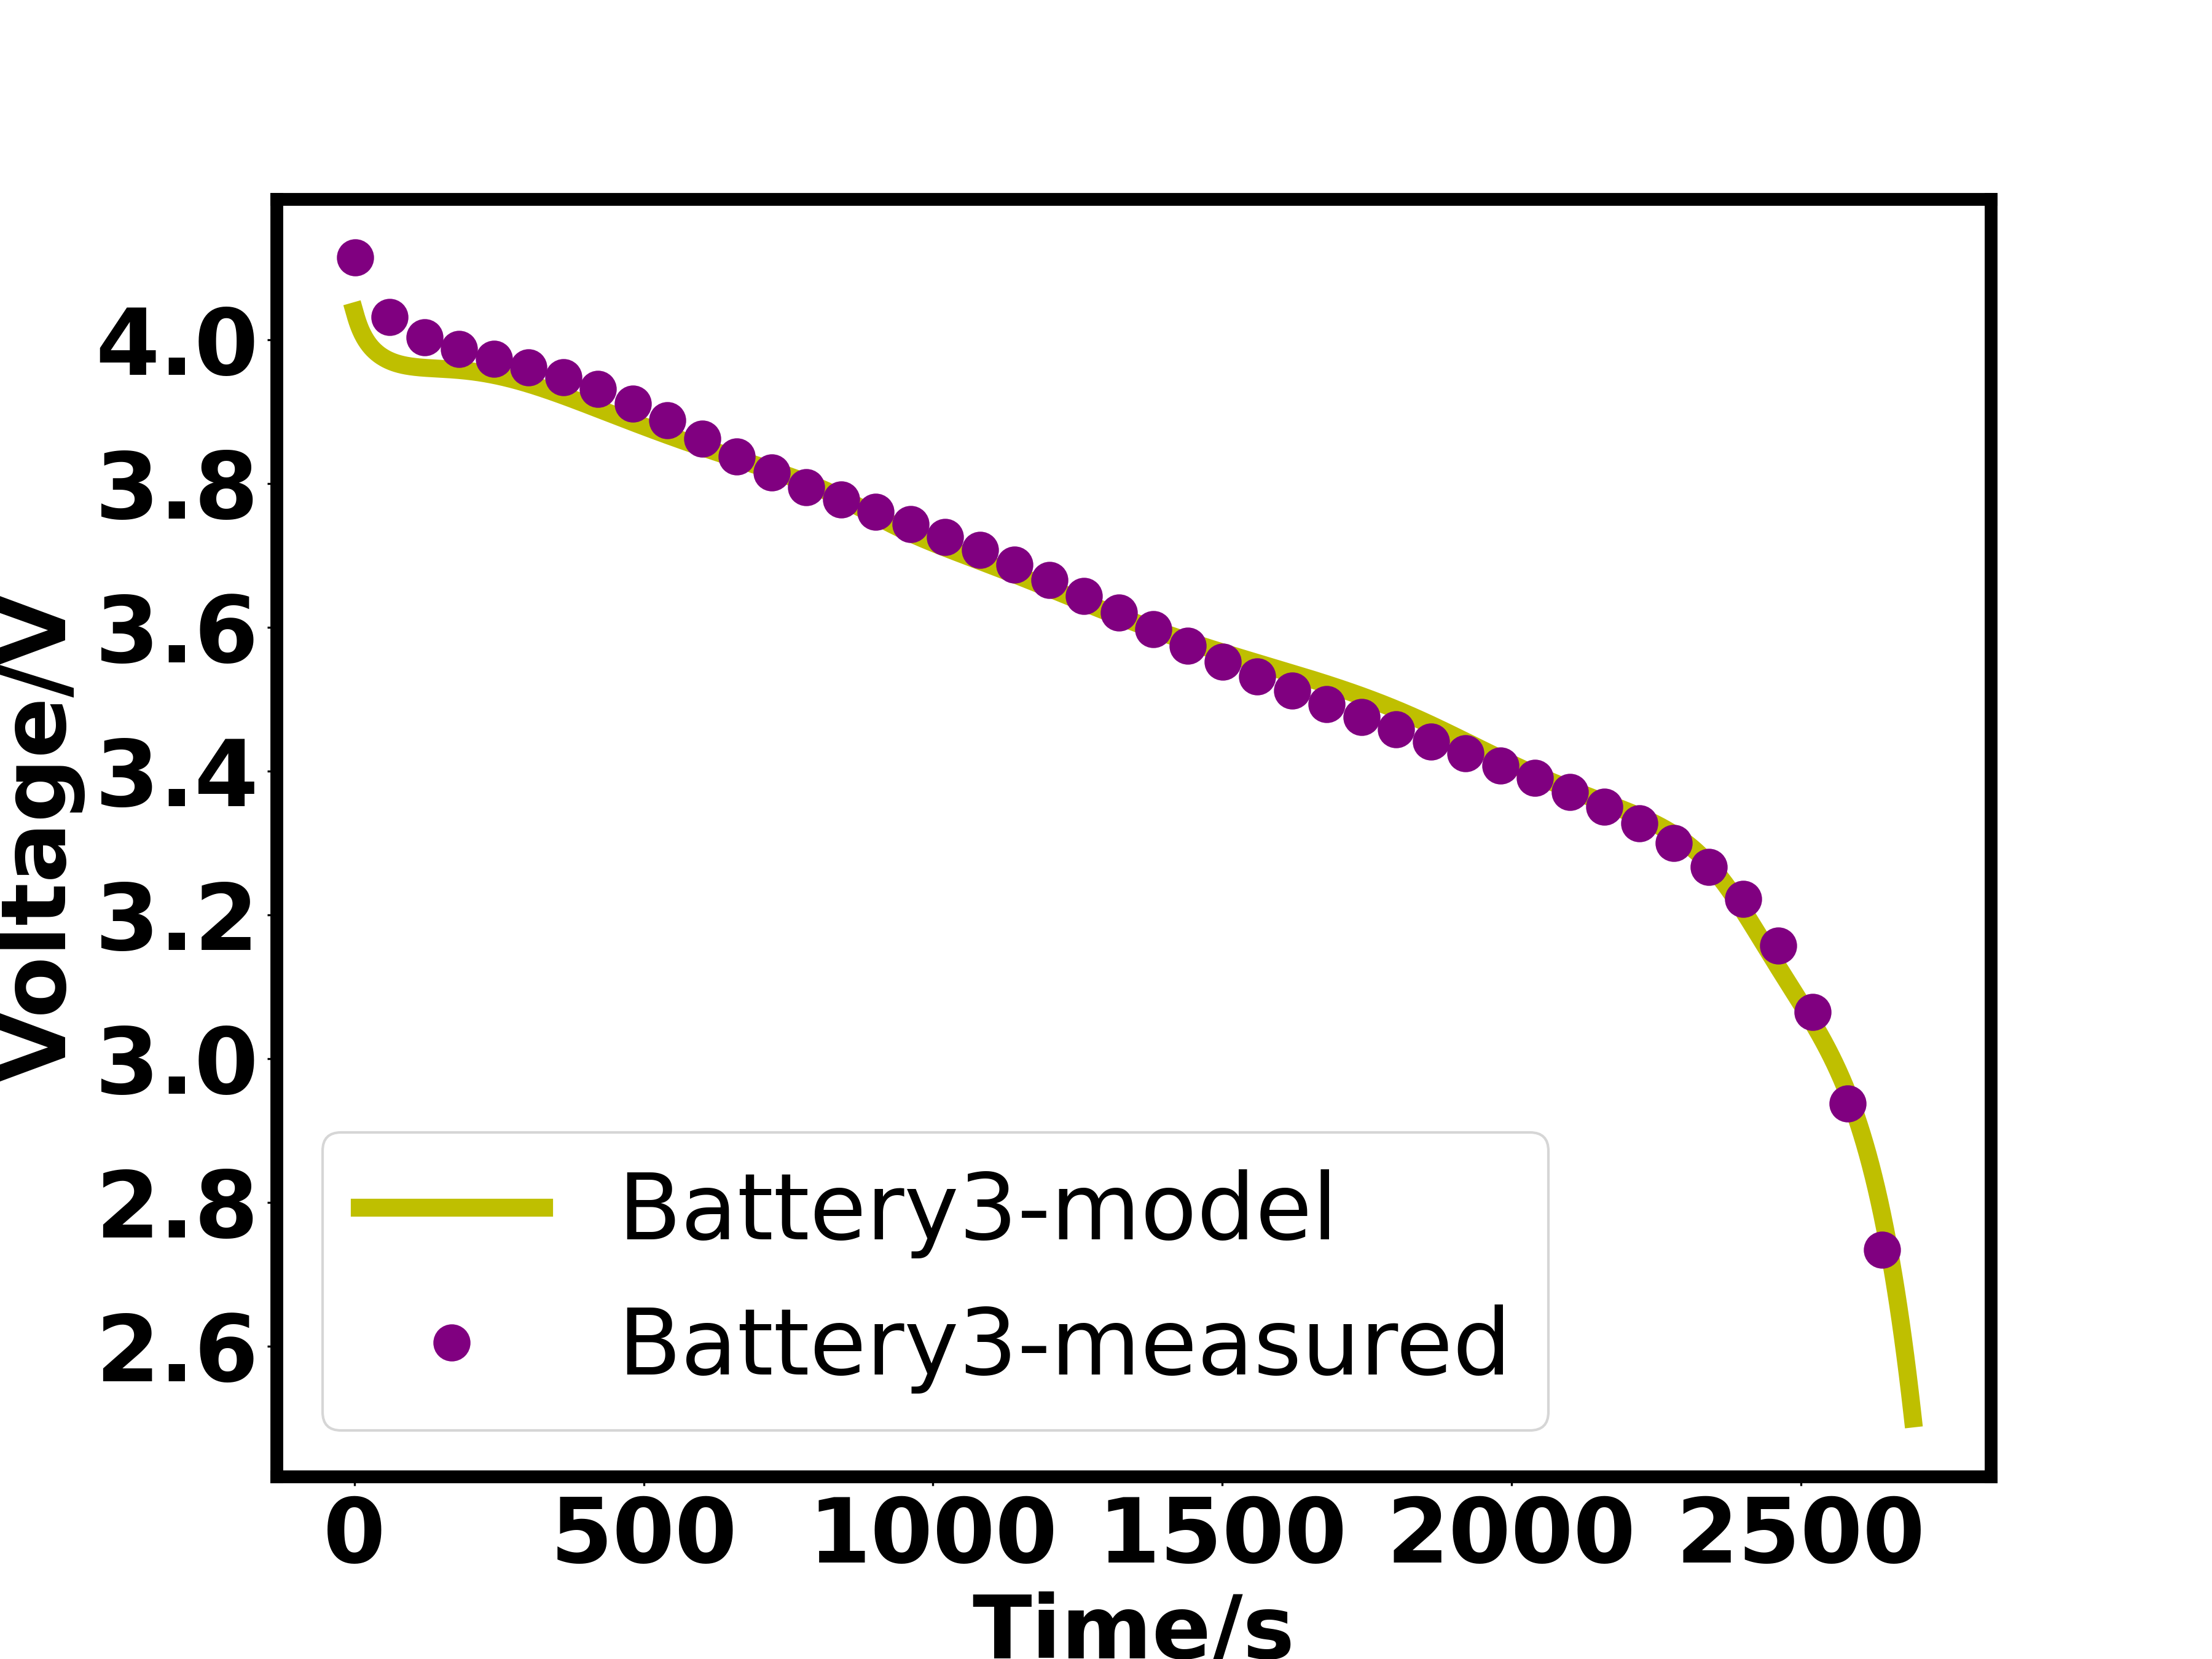
\includegraphics[width=\textwidth]{cell3_voltage_fit.png}
        \caption{}
    \end{subfigure}
    \hfill
    \begin{subfigure}[t]{0.24\textwidth}
        \centering
        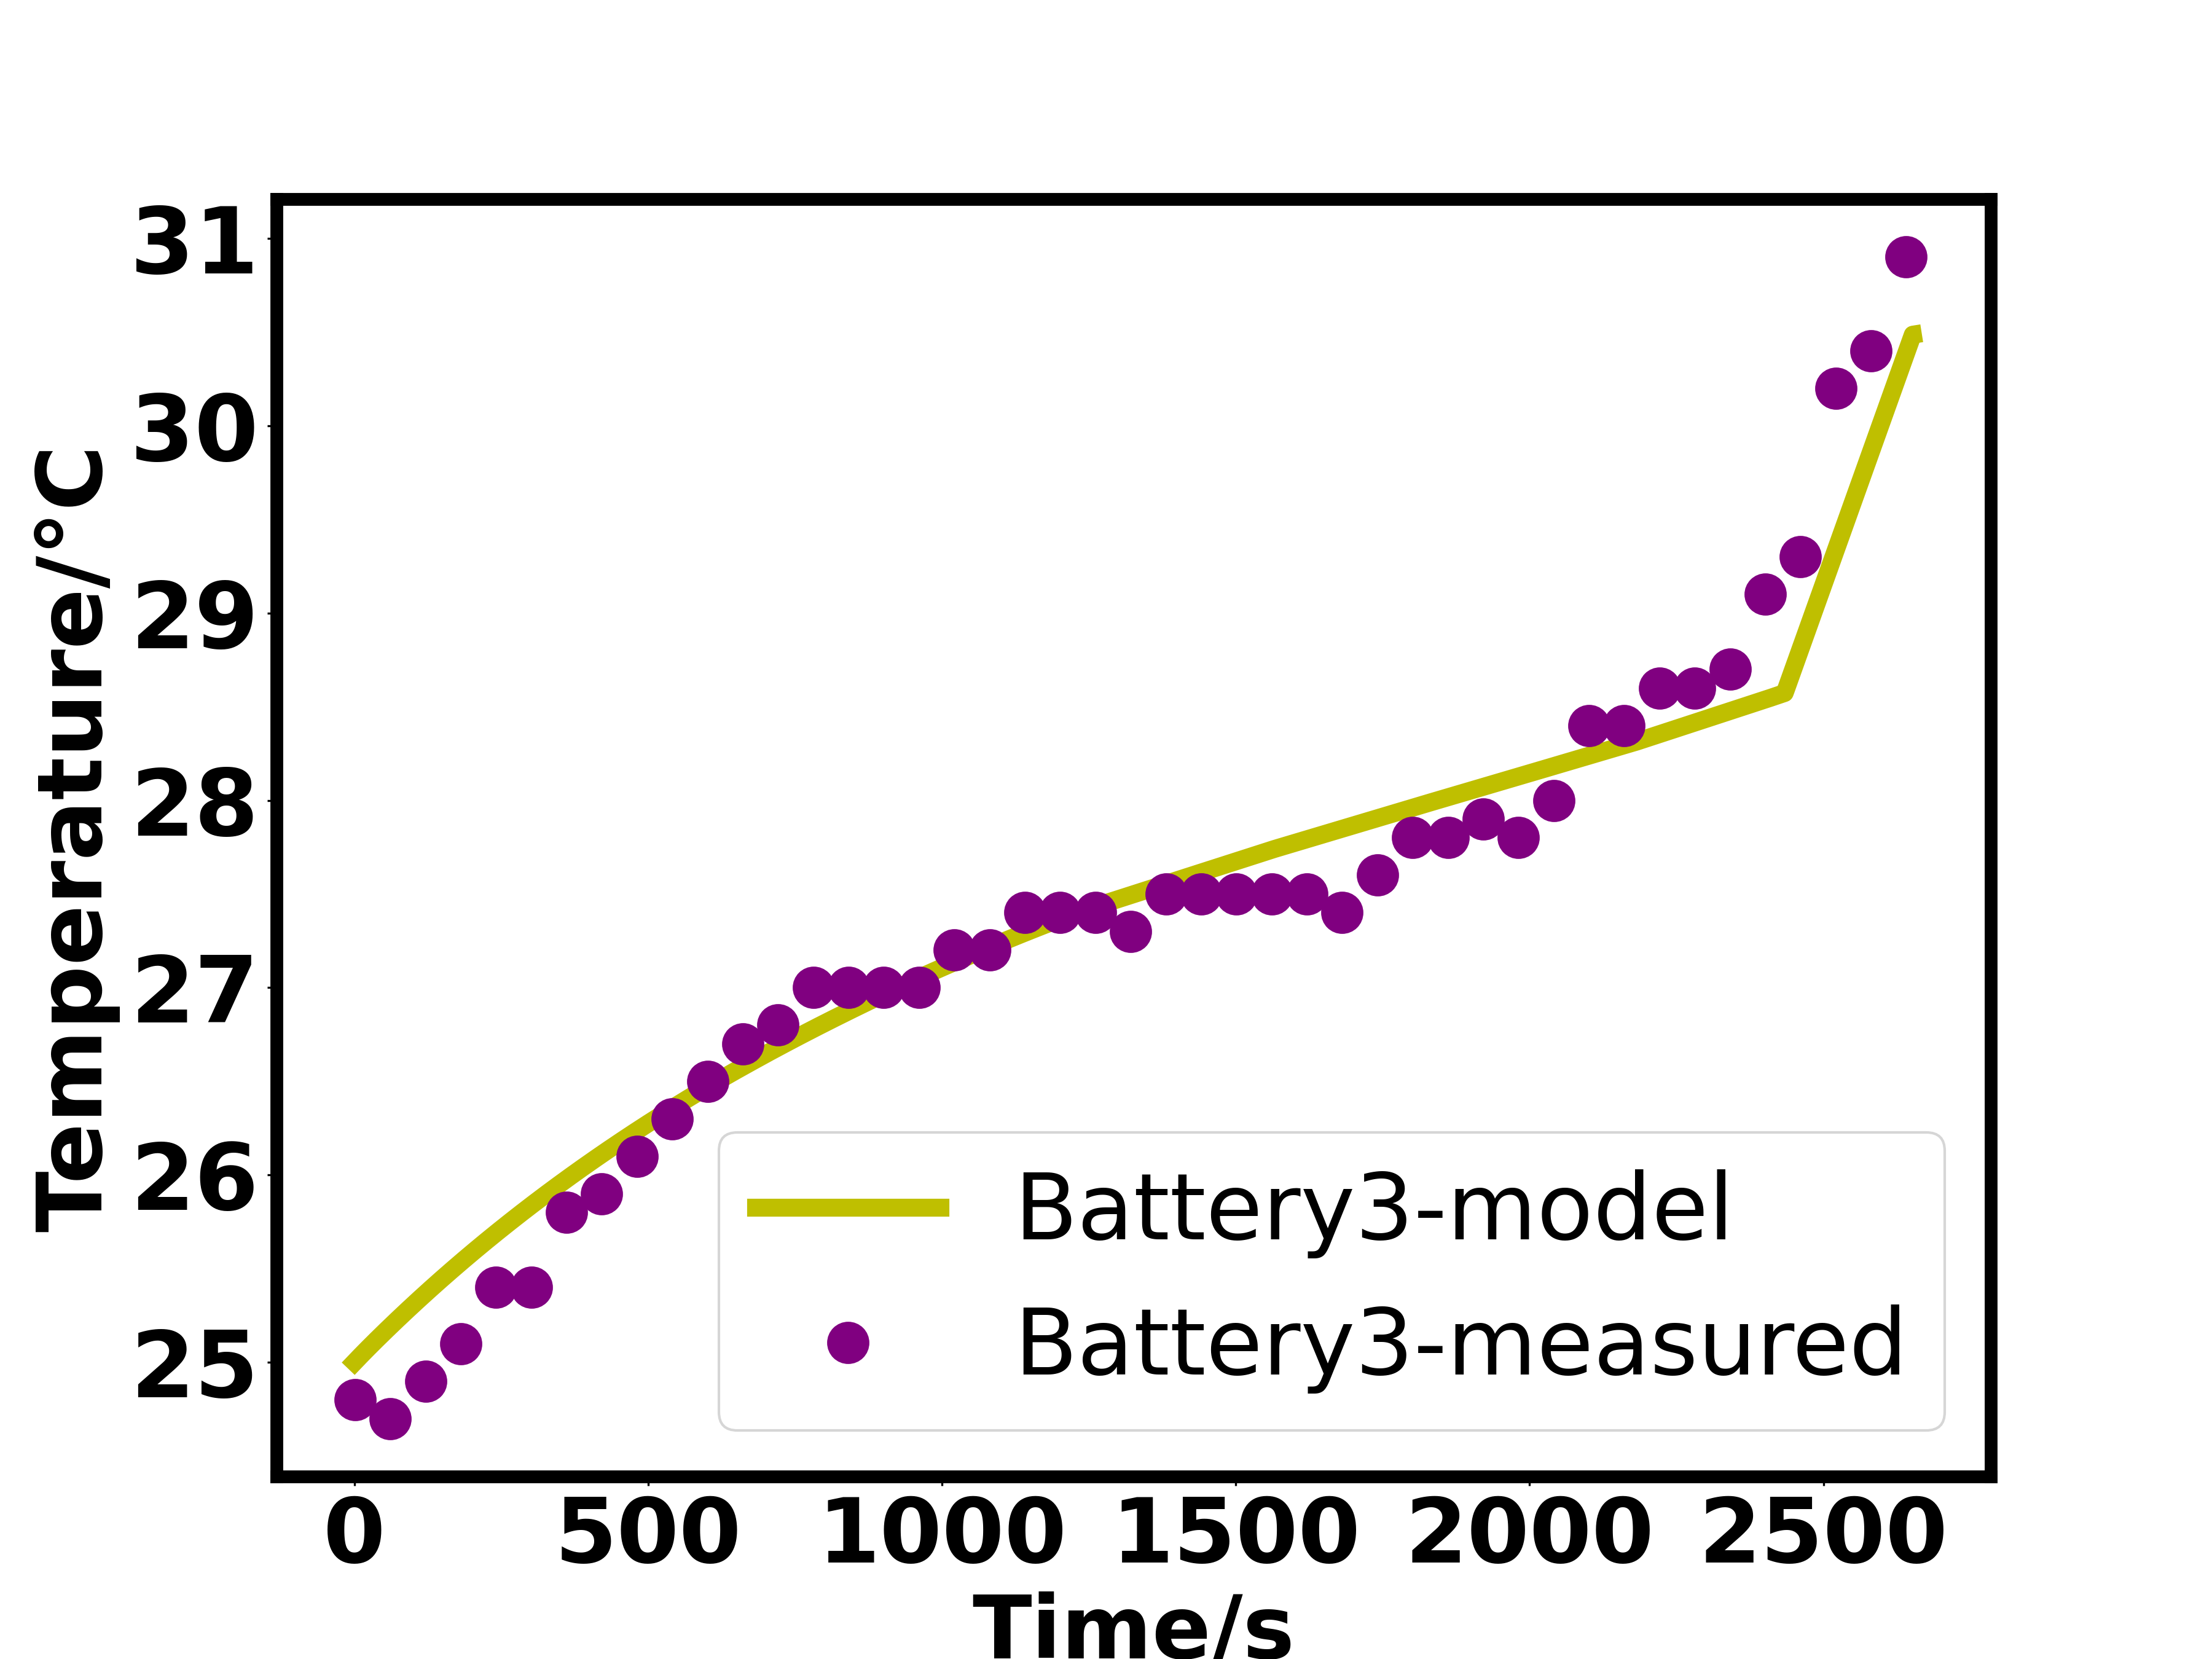
\includegraphics[width=\textwidth]{cell3_temperature_fit.png} 
        \caption{}
    \end{subfigure}

    \caption{Parameter identification results for Cell 3. (a) Electrochemical model parameter identification. (b) Thermal model parameter identification.}
    \label{battery3}
\end{figure}

\section{Results and Discussions}
\newrev{The performance of MBA-RL was evaluated using cell-specific models identified from three Samsung 40T 21700 cells, denoted as Cell 1, Cell 2, and Cell 3. The cells have a nominal capacity of 4000 mAh and a maximum discharge rate of 35 A. Voltage and temperature data were collected with the NEWARE CT-4008-5V20A-A platform shown in Fig.~\ref{fig:experiment_Schematic}. The identified SPMe models were used for policy training and evaluation under independently regulated charging channels.}

\begin{figure*}[htbp]
    \centering
        \begin{subfigure}[t]{0.32\textwidth}
        \centering
        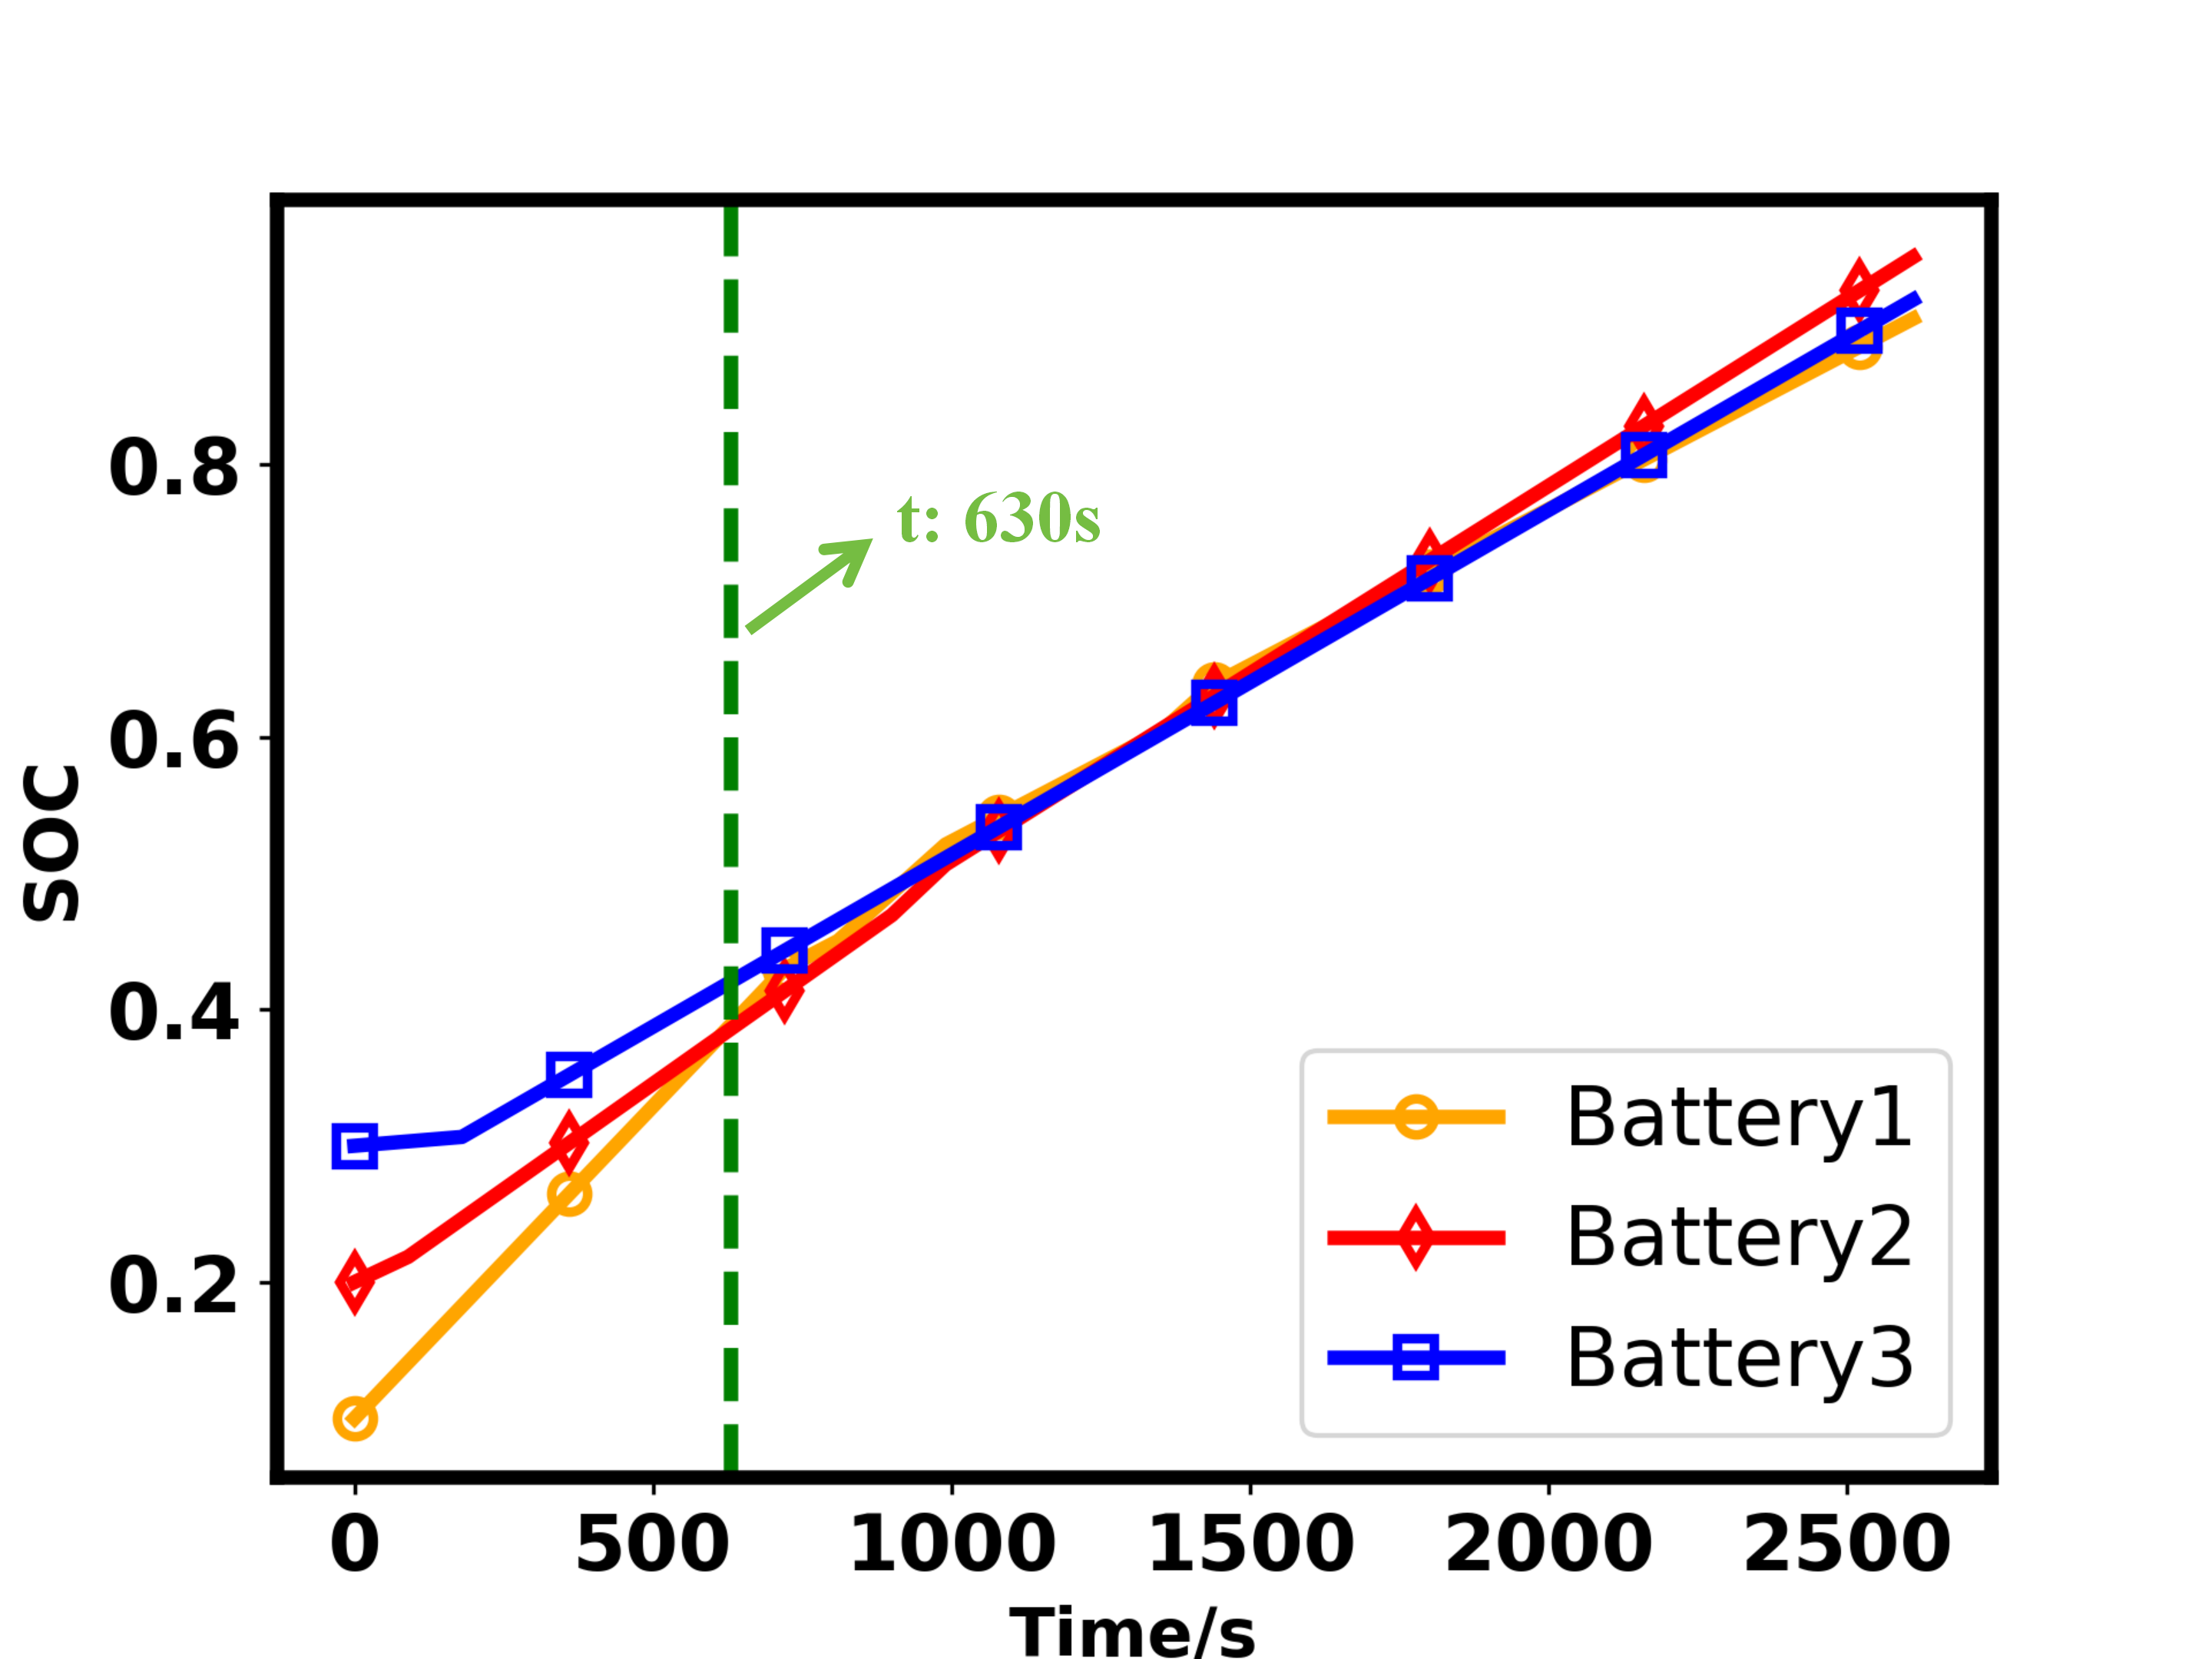
\includegraphics[width=\textwidth]{mba_rl_set_a.png}
        \caption{}
    \end{subfigure}
    \hfill
        \begin{subfigure}[t]{0.32\textwidth} 
        \centering
        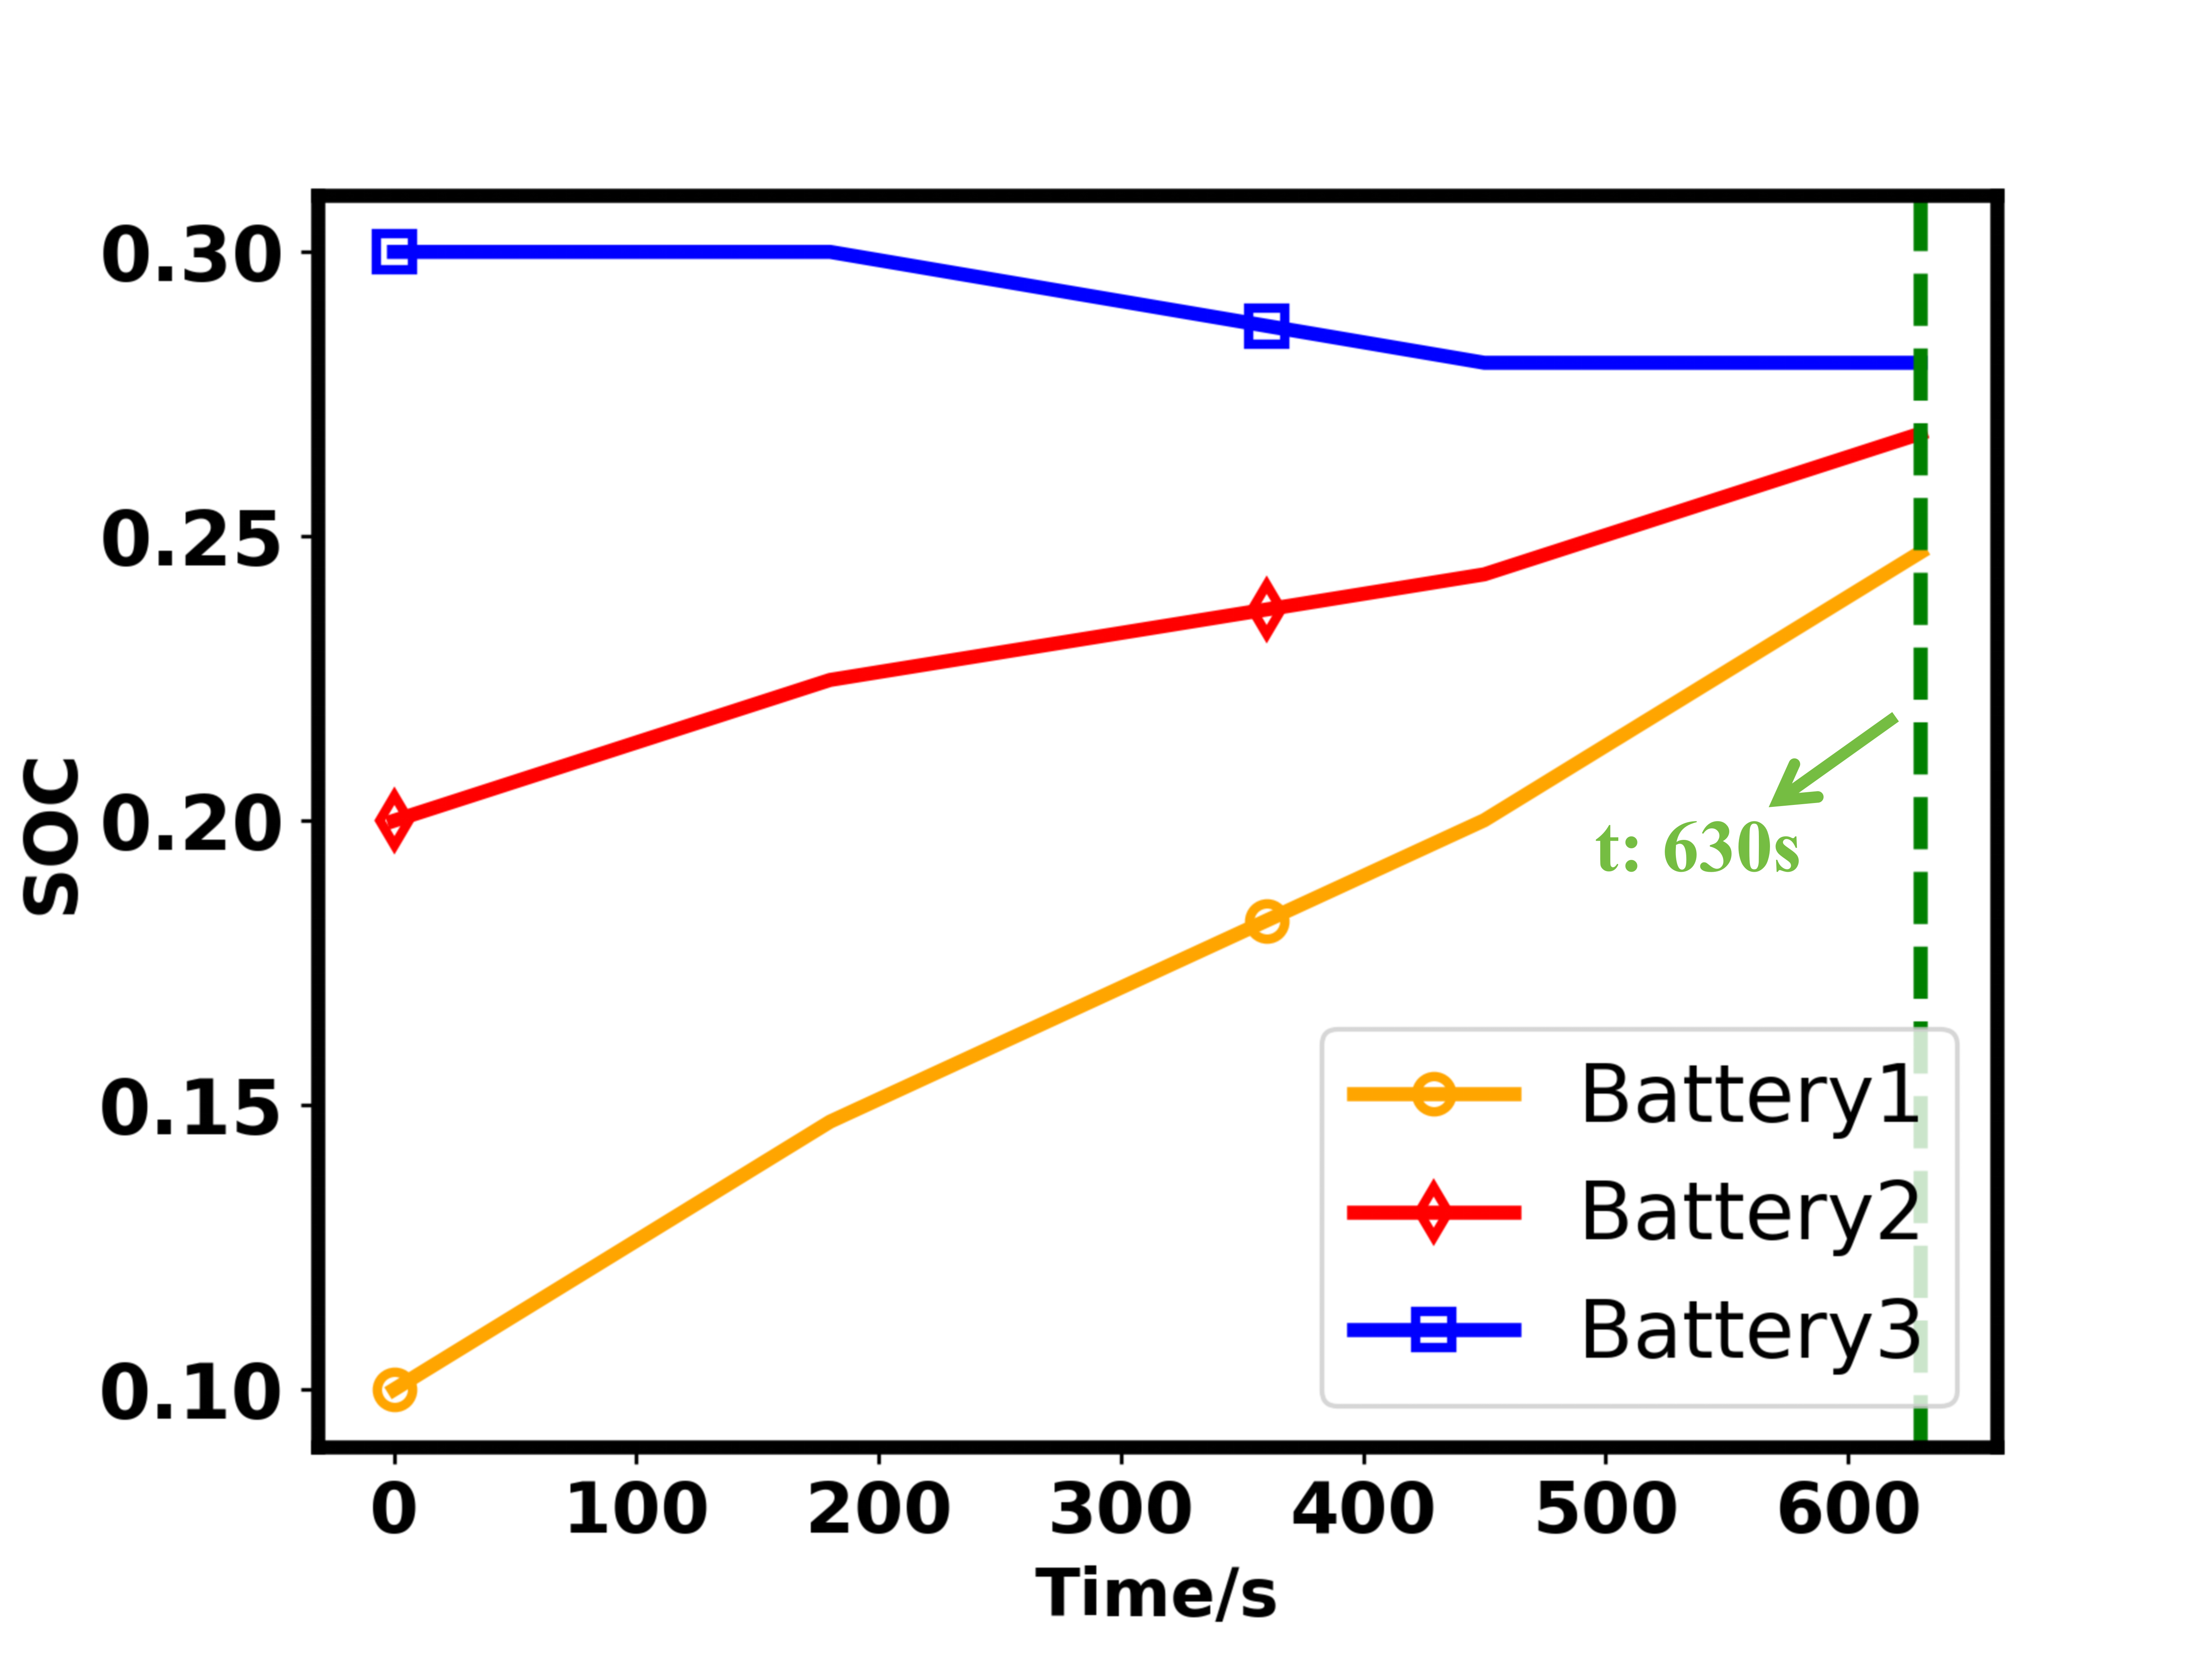
\includegraphics[width=\textwidth]{dql_set_a.png}
        \caption{}
    \end{subfigure}
    \hfill
        \begin{subfigure}[t]{0.32\textwidth} 
        \centering
        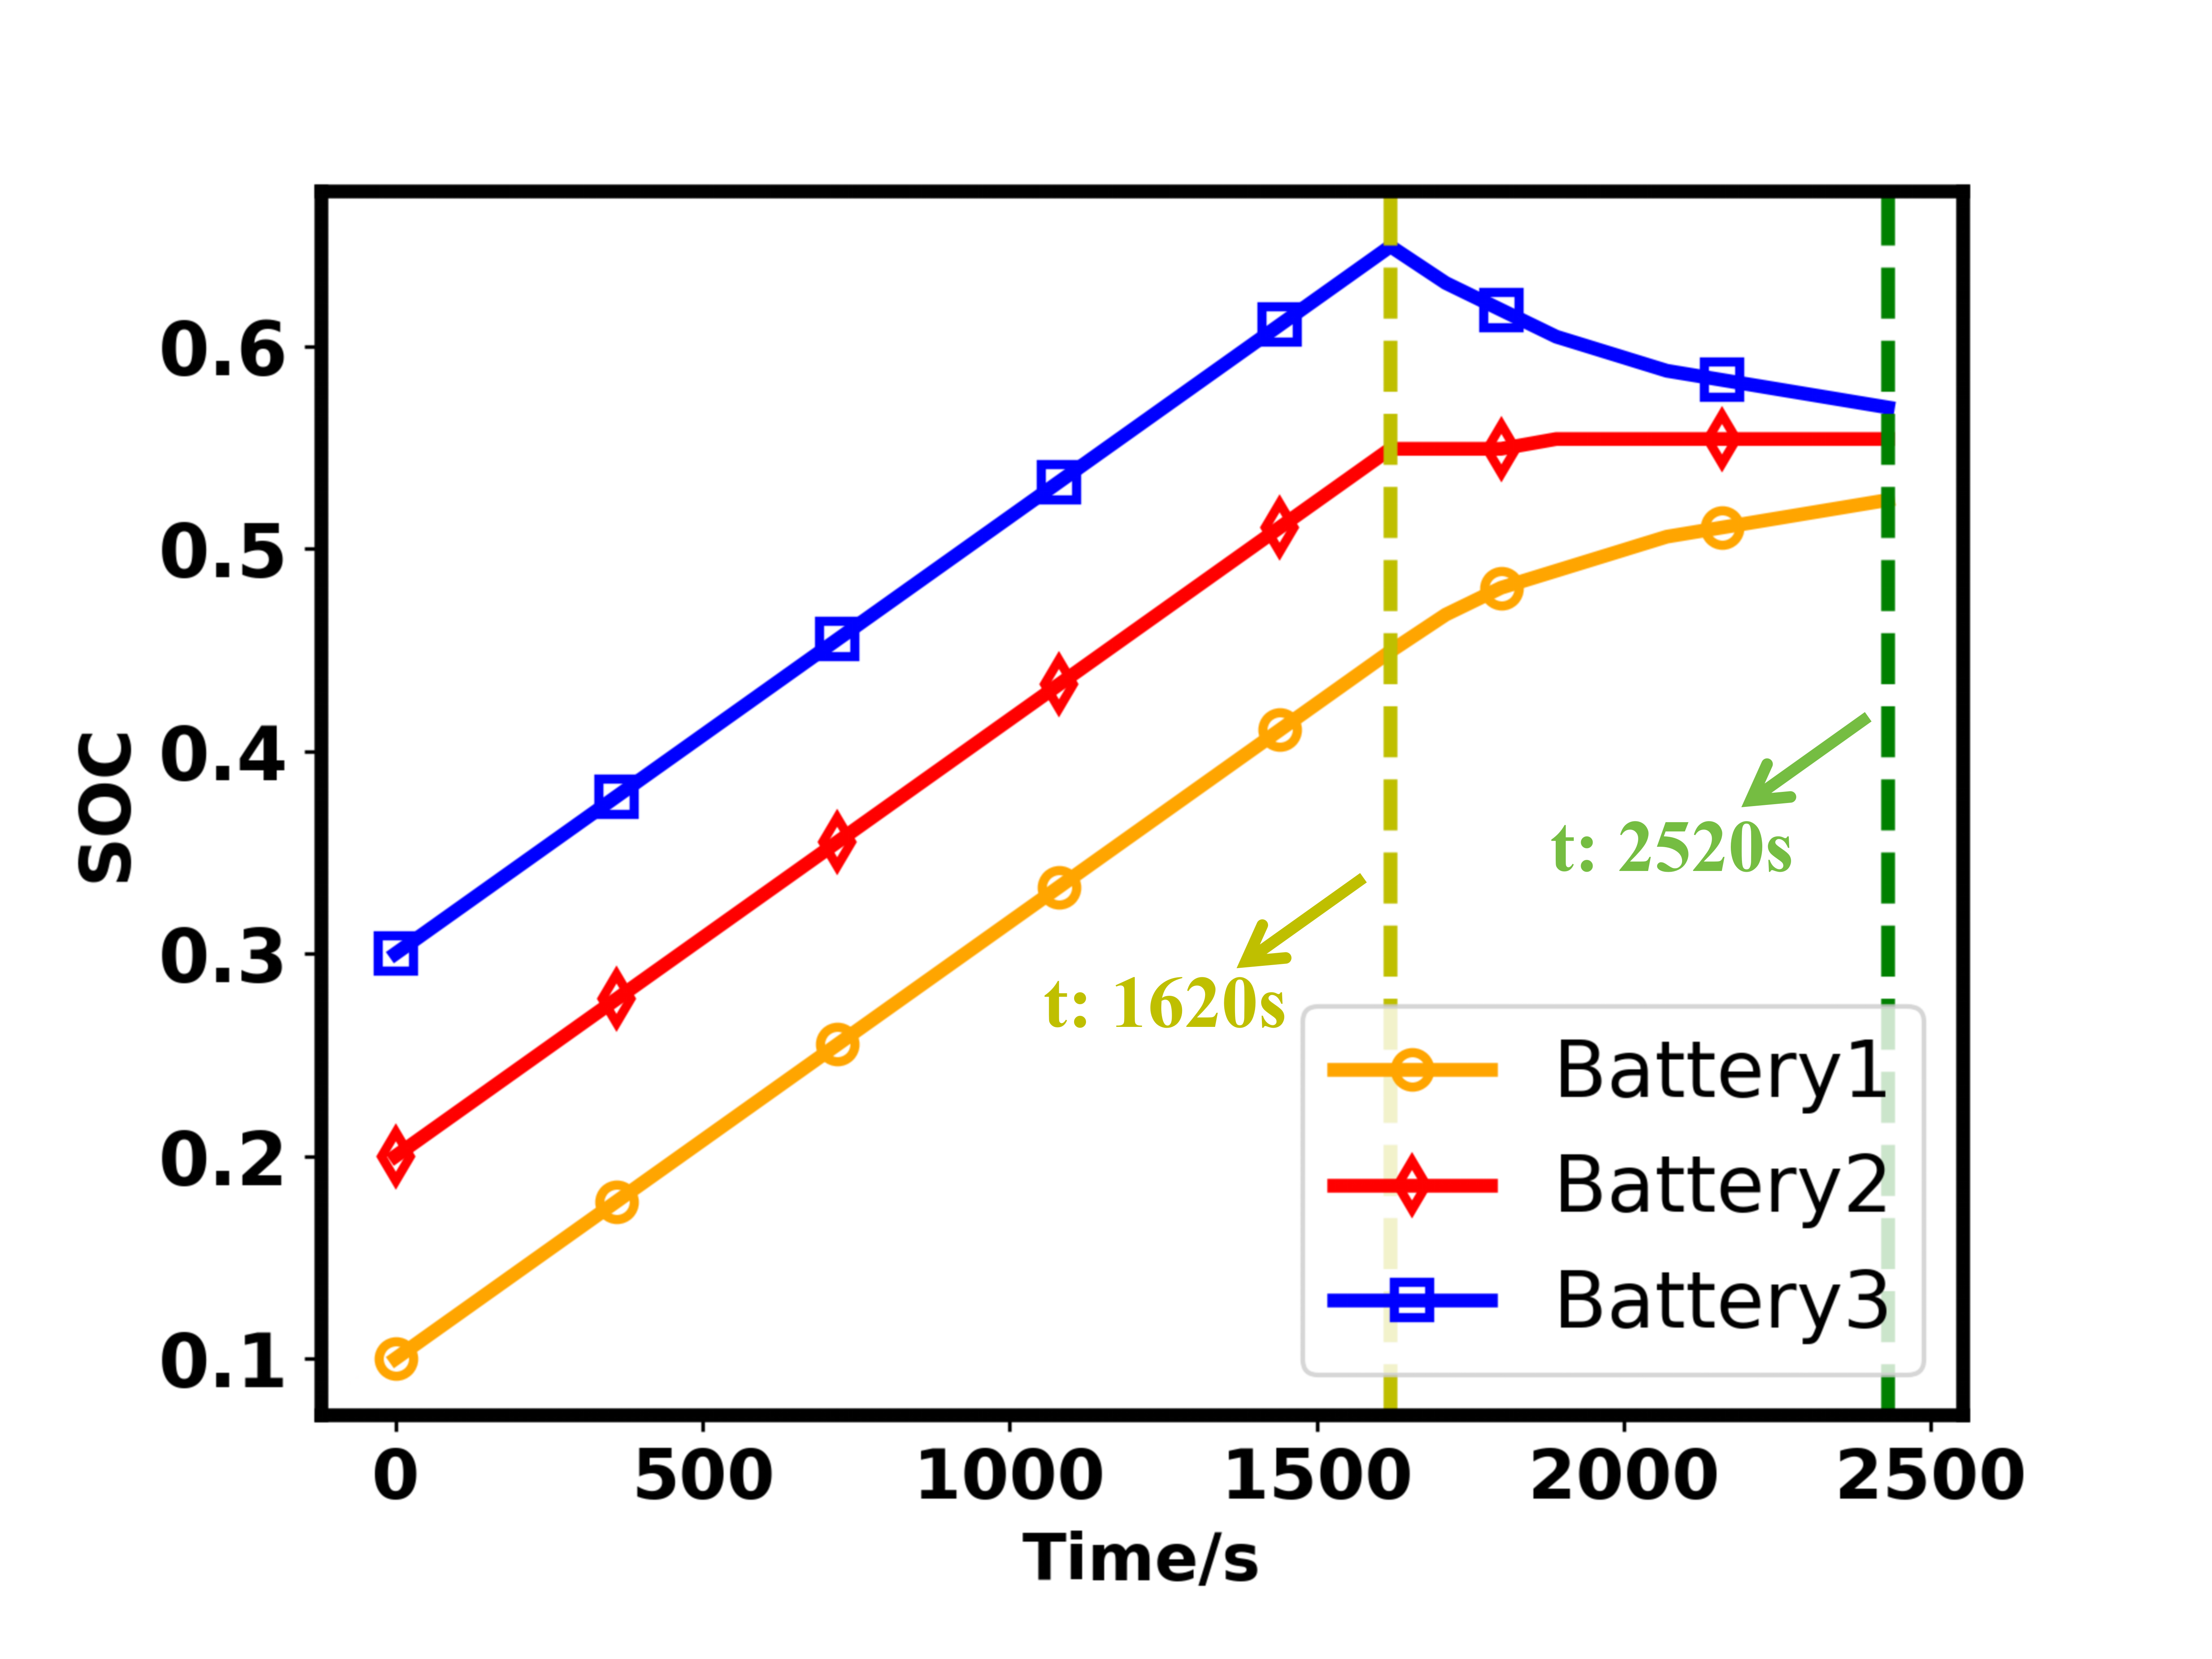
\includegraphics[width=\textwidth]{cc_cv_set_a.png}
        \caption{}
    \end{subfigure}

    \vspace{0.1cm}

    \begin{subfigure}[t]{0.32\textwidth}
        \centering
        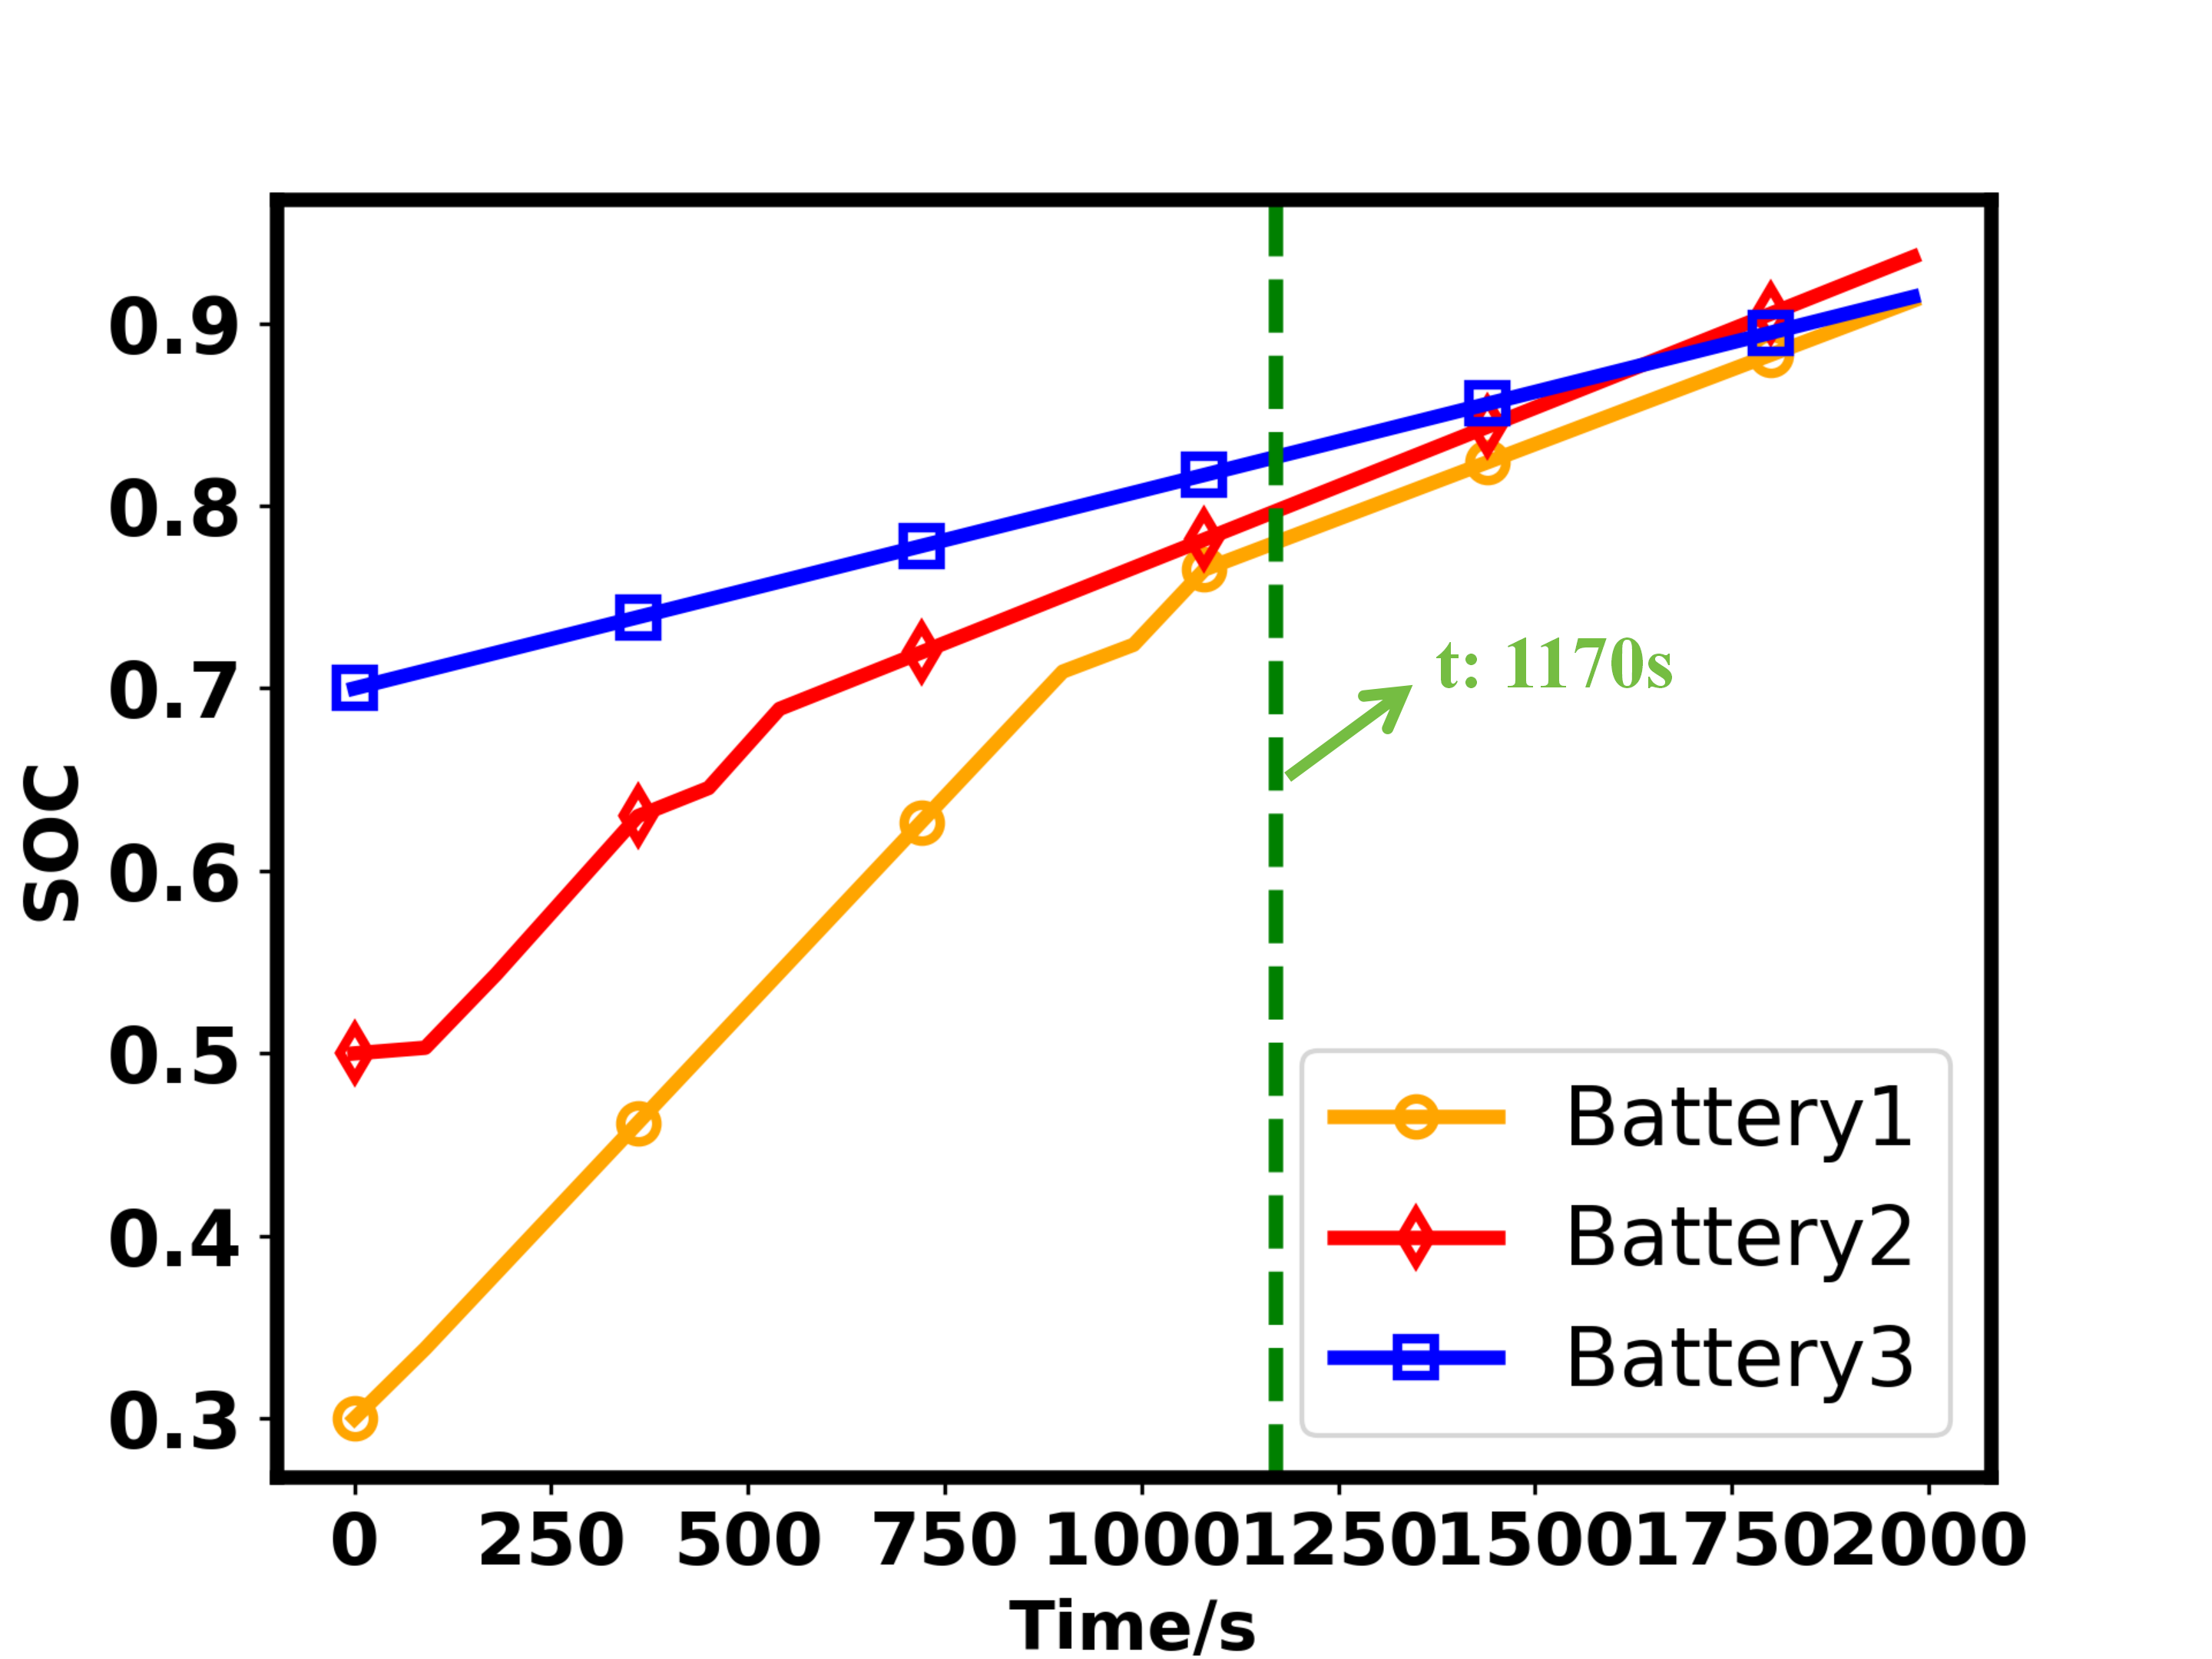
\includegraphics[width=\textwidth]{mba_rl_set_b.png}
        \caption{}
    \end{subfigure}
    \hfill
    \begin{subfigure}[t]{0.32\textwidth}
        \centering
        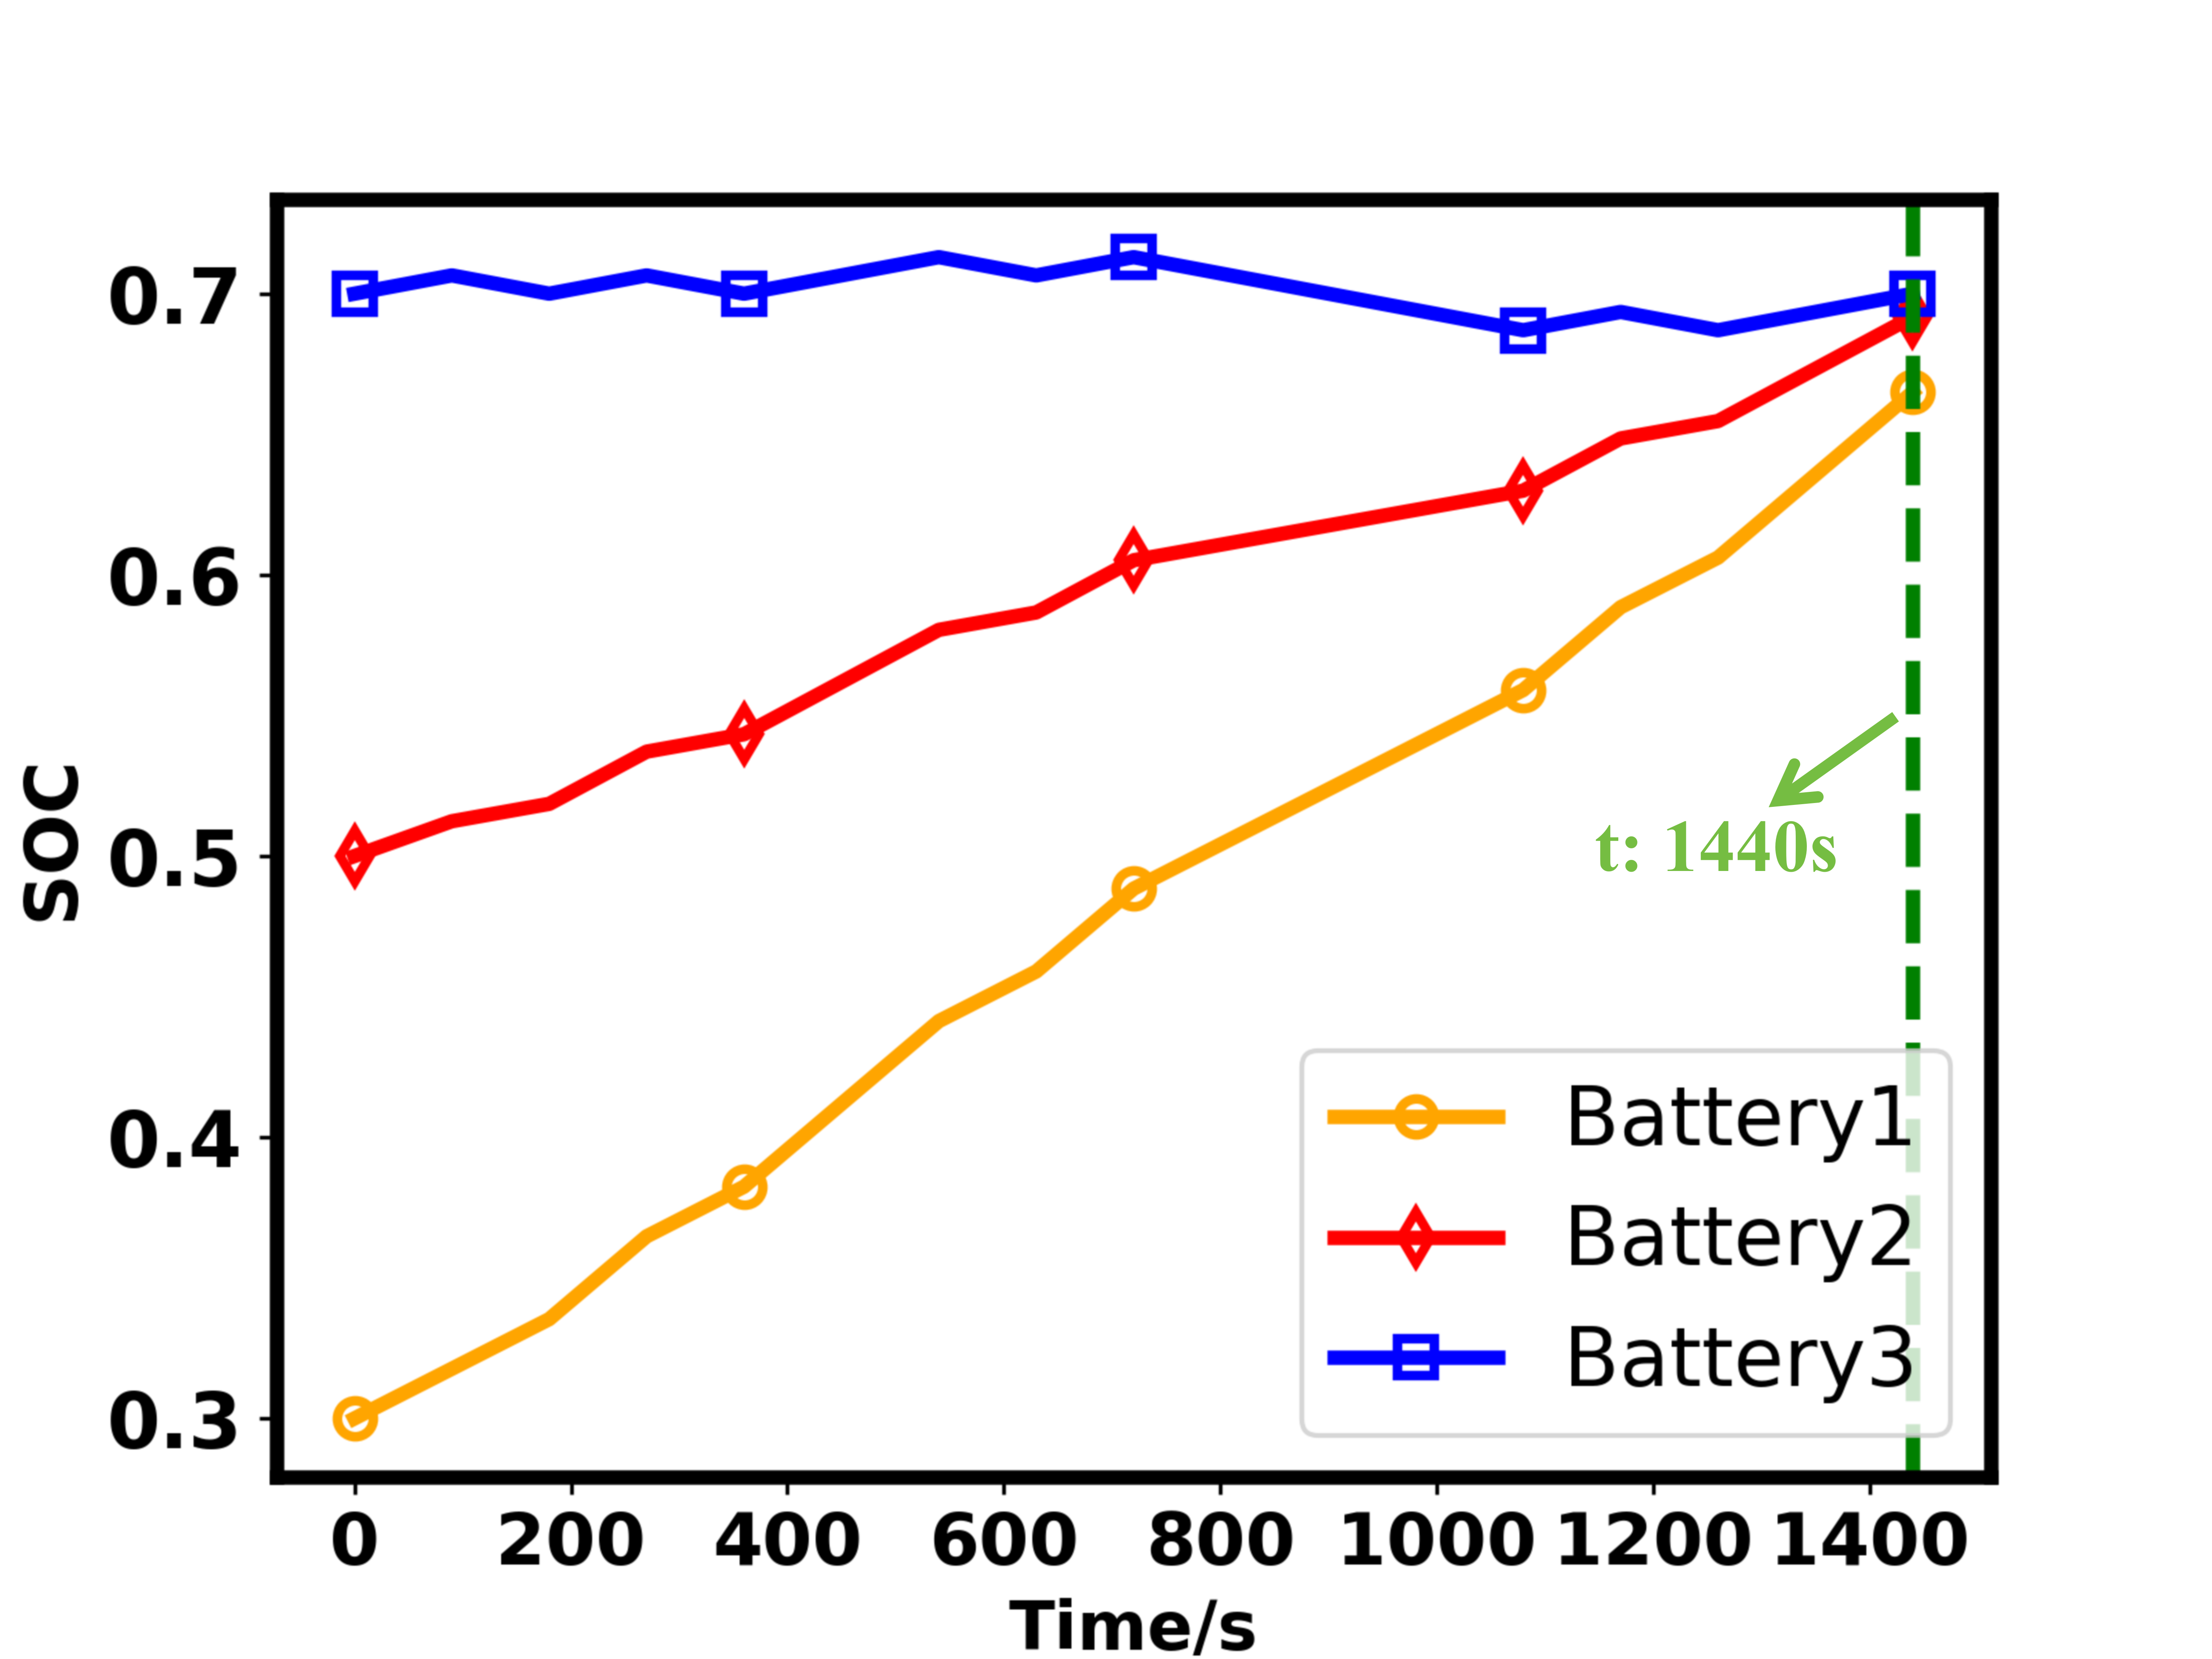
\includegraphics[width=\textwidth]{dql_set_b.png}
        \caption{}
    \end{subfigure}
    \hfill
    \begin{subfigure}[t]{0.32\textwidth} 
        \centering
        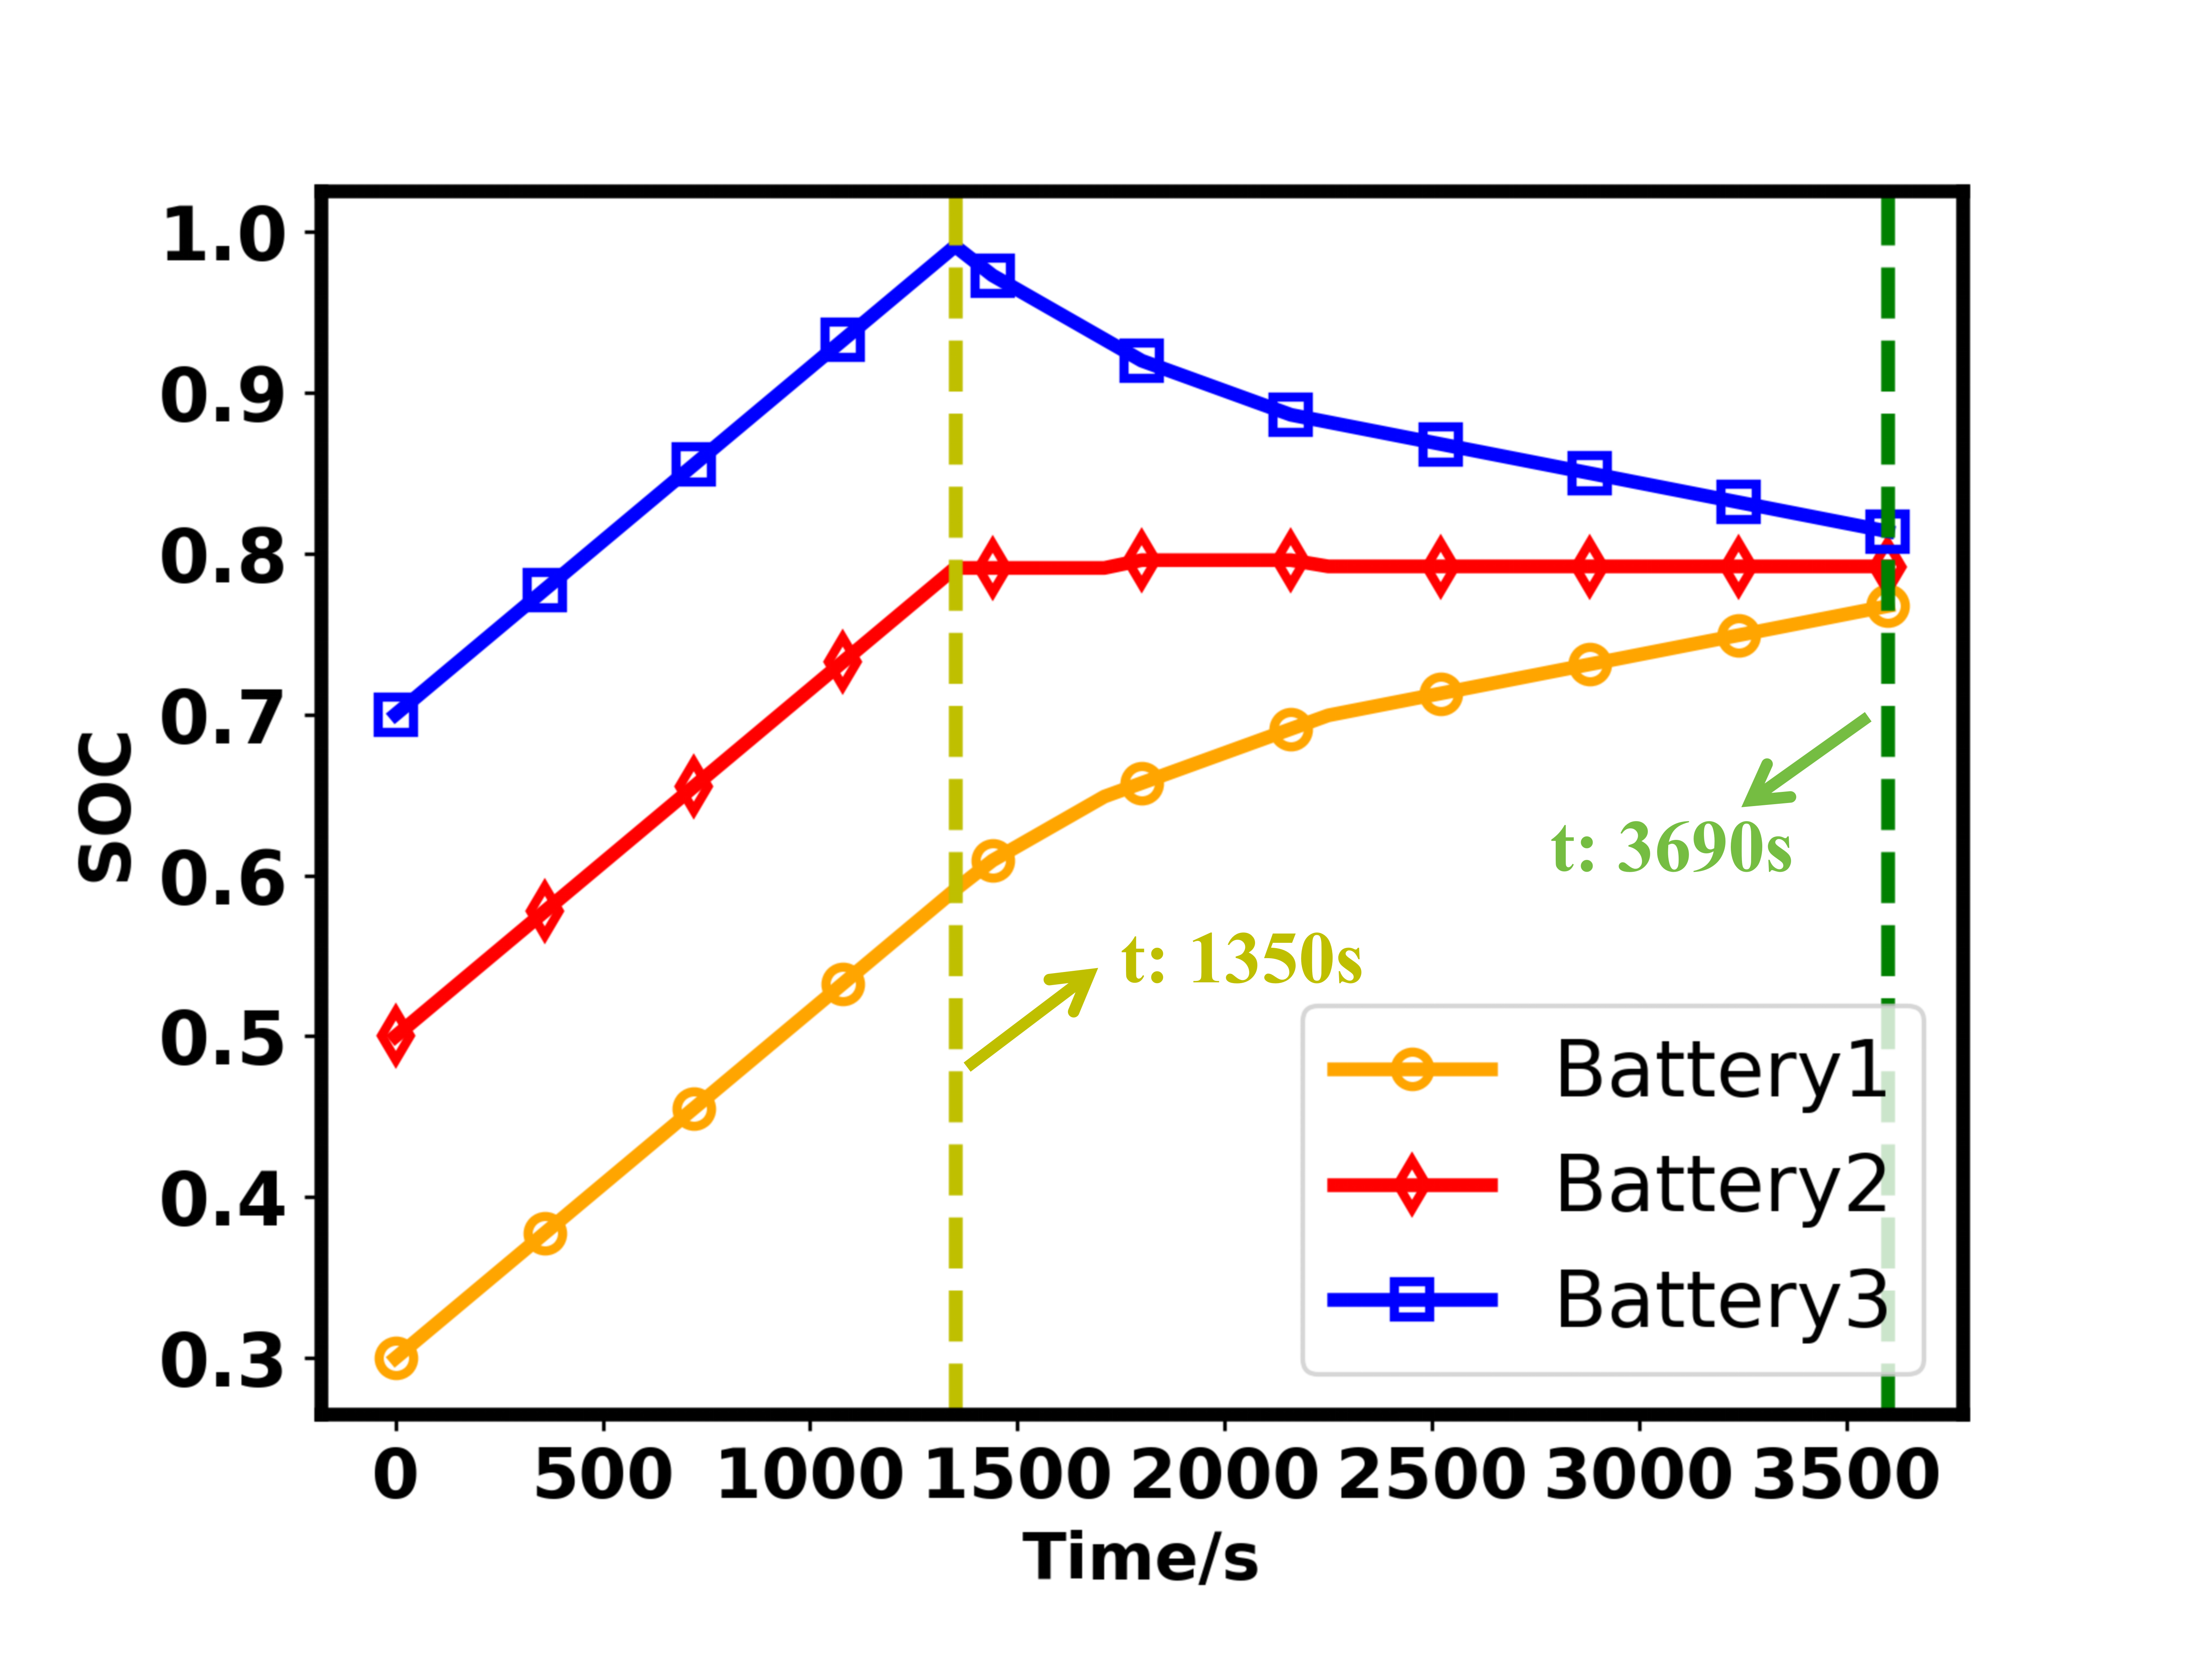
\includegraphics[width=\textwidth]{cc_cv_set_b.png}
        \caption{}
    \end{subfigure}

    \caption{Charging trajectories for MBA-RL, DQL, and CC-CV. The green dashed line indicates the first time at which $\sigma\leq\beta$, while the yellow dashed line marks the end of the CC phase. (a) MBA-RL in $Set\;A$. (b) DQL in $Set\;A$. (c) CC-CV in $Set\;A$. (d) MBA-RL in $Set\;B$. (e) DQL in $Set\;B$. (f) CC-CV in $Set\;B$.}
    \label{fig:overall_figure}
\end{figure*}

\subsection{\newrev{Parameter Identification for Cells at Different Aging Levels}}
\newrev{To obtain cells at different aging levels, Cells 2 and 3 were cycled for 140 and 260 charge-discharge cycles, respectively. The voltage and temperature measurements in Fig.~\ref{fig:three_aging} were then used to identify cell-specific SPMe parameters with PSO \cite{28}. Figs.~\ref{battery1}-\ref{battery3} compare the identified models with the measurements. The RMSEs in Table I show that the models reproduce the measured voltage and temperature profiles under the considered identification conditions.}


\begin{table}[t]
\centering
\caption{RMSEs for the three identified cells}
\begin{tabular}{c c c c}
\noalign{\hrule height 0.3mm}
\textbf{} & Cell 1 & Cell 2 & Cell 3 \\
\noalign{\hrule height 0.3mm}
$V_{RMSE}$ & 0.026 & 0.035 & 0.029 \\
\hline
$T_{RMSE}$ & 0.068 & 0.091 & 0.093 \\
\hline
\noalign{\hrule height 0.3mm}
\end{tabular}
\end{table}

\begin{table}[!t]
\centering
\color{red}
\caption{\newrev{Control and evaluation settings}}
\label{tab:experimental_settings}
\scriptsize
\setlength{\tabcolsep}{3pt}
\renewcommand{\arraystretch}{1.03}
\begin{tabular}{@{}p{0.31\columnwidth}p{0.63\columnwidth}@{}}
\toprule
\textbf{Setting} & \textbf{Value} \\
\midrule
Battery model & SPMe with lumped thermal model \\
Current command & $0$--$7.5$ A, 0.5 A step, 90 s interval \\
Task criterion & $SOC_i\geq0.90$, $\sigma\leq0.02$, 5400 s horizon, 270 s hold \\
Operating limits & $V\leq4.2$ V, $T\leq309$ K, $SOC\leq0.95$ \\
Safety margins & 0.03 V and 1 K \\
Ambient temperature & 298.15 K \\
\bottomrule
\end{tabular}
\end{table}

\begin{table}[t]
\centering
\caption{\newrev{Battery pack SOC vectors at the first balance-attainment point}}
\label{tab:soc_vectors}
\begin{tabular}{c|c|c}
\hline
\noalign{\hrule height 0.2mm}
\textbf{Method} & \textbf{Initial SOC (\%)} & \textbf{\newrev{SOC at first balance (\%)}} \\
\hline
\noalign{\hrule height 0.2mm}
\multirow{2}{*}{MBA-RL} & $[10, 20, 30]^\text{T}$ & $[91.66, 94.18, 92.15]^\text{T}$ \\
                        & $[30, 50, 70]^\text{T}$ & $[91.23, 93.62, 91.41]^\text{T}$ \\ \hline
\multirow{2}{*}{DQL} & $[10, 20, 30]^\text{T}$ & $[24.72, 26.81, 28.05]^\text{T}$ \\
                        & $[30, 50, 70]^\text{T}$ & $[66.50, 69.18, 70.00]^\text{T}$ \\ \hline
\multirow{2}{*}{CC-CV}  & $[10, 20, 30]^\text{T}$ & $[52.41, 55.42, 56.97]^\text{T}$ \\
                        & $[30, 50, 70]^\text{T}$ & $[76.74, 79.21, 81.38]^\text{T}$ \\ \hline
                        \noalign{\hrule height 0.2mm}
\end{tabular}
\end{table}



\subsection{Performance Evaluation of MBA-RL}
\newrev{The battery models were implemented in PyBaMM \cite{29} and updated with the identified parameters. The policies were trained through interaction with these models, and the selected weights were frozen during testing. A task was completed when every cell reached the reference SOC and the SOC standard deviation remained below the balancing threshold for 270 s without violating the safety limits. The two initial SOC vectors $Set\; A=[10,20,30]^\mathrm{T}$ and $Set\; B=[30,50,70]^\mathrm{T}$ in Fig.~\ref{fig:overall_figure} and Table~\ref{tab:soc_vectors} are retained as illustrative cases.}

\newrev{MBA-RL regulates the charging current of each cell at every decision step according to its local state and the pack state. In the implemented comparisons, DQL additionally controls a cell-to-cell energy-transfer topology, while the CC-CV baseline activates the topology during the CV phase.}

\newrev{Fig.~\ref{fig:overall_figure} is used to explain the charging trajectories rather than to rank the methods by the first balance-attainment time alone. MBA-RL and DQL first satisfy $\sigma\leq\beta$ earlier than CC-CV in the two illustrative cases, but DQL and CC-CV do so before every cell reaches the terminal SOC target. In the implemented comparison, CC-CV follows its two-stage profile and does not adapt the current with the temperature-aware predictive screen used by MBA-RL. MBA-RL instead applies the same voltage, temperature, and SOC limits throughout charging.}

\newrev{Table~\ref{tab:soc_vectors} shows that MBA-RL first reaches $\sigma\leq\beta$ after all cells have passed the reference SOC, whereas the comparison methods first reach this condition at lower SOC values. The main performance assessment therefore uses task completion, time score, accumulated SOC imbalance $\int\sigma(t)\,\mathrm{d}t$, and constraint satisfaction rather than the first balance-attainment time.}

\subsubsection{\newrev{Safety-Constrained Execution}}

\newrev{To distinguish execution screening from safety-aware training, the screen was first applied only to a frozen policy. It increased constraint satisfaction from 3/52 to 52/52 and task completion from 1/52 to 35/52. Using the same mechanism during training completed all 52 tests and reduced accumulated SOC imbalance, $\int\sigma(t)\,\mathrm{d}t$, from 469.97 to 197.34 SOC fraction s. The screen therefore rejects inadmissible actions, while its inclusion during training improves charging progress under the same constraints.}

\subsubsection{\newrev{Comparative Charging Performance}}

\begin{table}[!t]
\centering
\color{red}
\caption{Learned-method performance over unseen initial-SOC conditions}
\label{tab:modern_baselines}
\footnotesize
\renewcommand{\arraystretch}{1.12}
\begin{tabular*}{0.98\columnwidth}{@{\extracolsep{\fill}}l c c@{}}
\toprule
\textbf{Method} & \textbf{Time score (s)} & $\boldsymbol{\int\sigma\,\mathrm{d}t}$ \\
 & & \textbf{(SOC fraction s)} \\
\midrule
\multicolumn{3}{@{}l}{\textit{Discrete-action methods}} \\
MBA-RL & $2701.50\pm919.80$ & $205.42\pm57.03$ \\
Shared IQL & $2641.50\pm439.42$ & $235.17\pm69.76$ \\
Centralized DQN & $2673.00\pm73.98$ & $230.35\pm24.20$ \\
Discrete MAPPO & $2340.00\pm347.96$ & $200.83\pm60.75$ \\
\addlinespace[1pt]
\multicolumn{3}{@{}l}{\textit{Continuous-action methods}} \\
Continuous MAPPO & $2698.50\pm154.65$ & $240.36\pm27.58$ \\
SAC & $2173.50\pm157.09$ & $156.04\pm30.74$ \\
\bottomrule
\end{tabular*}
\end{table}

\newrev{The learned methods were evaluated in 60 runs covering 12 fixed unseen initial-SOC conditions and five independent training runs. Failed tasks receive a time score of 5670 s, and $\pm$ denotes the standard deviation across the five training-run means. All methods completed 60/60 evaluations except continuous MAPPO, which completed 59/60. Compared with shared IQL and centralized DQN, two value-based baselines using the same discrete current set, MBA-RL reduces accumulated SOC imbalance by 12.65\% and 10.82\%, respectively. Discrete MAPPO and SAC achieve lower numerical scores in Table~\ref{tab:modern_baselines}. MBA-RL jointly realizes independently regulated cell charging, topology-free pack balancing, and model-based safety screening within a unified framework.}

\begin{figure}[!t]
    \centering
    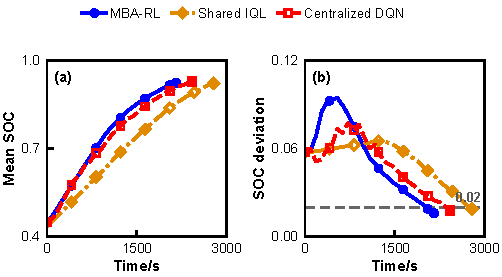
\includegraphics[width=\columnwidth]{comparative_charging_discrete.pdf}
    \caption{\newrev{Discrete-action charging trajectories for one unseen initial-SOC condition. (a) Pack mean SOC. (b) SOC standard deviation. MBA-RL, shared IQL, and centralized DQN use the same candidate-current set, initial SOC vector $[0.4203,0.3962,0.5280]^\mathrm{T}$, and ambient temperature of 25~$^\circ$C. Only the charge phase is displayed; the required 270 s terminal hold is evaluated but omitted. The dashed line denotes $\beta=0.02$.}}
    \label{fig:discrete_trajectories}
\end{figure}

\newrev{Fig.~\ref{fig:discrete_trajectories} compares MBA-RL with shared IQL and centralized DQN under the same discrete action authority. MBA-RL enters the target region earlier than shared IQL and reaches a smaller final SOC dispersion than centralized DQN in this representative case. Aggregate results over all unseen cases are reported in Table~\ref{tab:modern_baselines}.}

\subsubsection{\newrev{Ablation and Sensitivity Analysis}}

\newrev{We next ablate the main architectural and reward-design components and evaluate representative operating variations and pack sizes.}

\begin{figure}[!b]
    \centering
    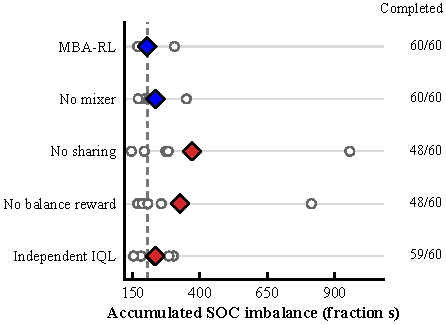
\includegraphics[width=\columnwidth]{component_ablation.pdf}
    \caption{\newrev{Key component ablations over 12 unseen conditions and five independent training runs. Open circles show the accumulated SOC imbalance for each training run, and diamonds show the five-run means; lower values indicate better balance. The dashed line marks the MBA-RL mean, and the right-hand labels give completed evaluations.}}
    \label{fig:component_ablation}
\end{figure}

\newrev{Removing parameter sharing or the balancing reward causes one complete training run to fail, reducing task completion from 60/60 to 48/60 and increasing the mean accumulated SOC imbalance by 80.47\% and 59.07\%, respectively. Removing the mixing network retains 60/60 completion but increases the imbalance by 14.48\%. These results identify parameter sharing and the balancing objective as the main contributors to training consistency in the tested three-cell task.}

\newrev{The frozen policy completes all 100 tests under the specified $\pm10\%$ parameter variations, fixed sensor bias, a 15~$^\circ$C ambient condition, and a 30\% reduction in available current. Completion decreases under observation noise, a one-decision delay, and ambient temperatures of 34--35~$^\circ$C. Thus, the observed robustness is limited mainly to the examined model and actuation variations.}

\newrev{The same MBA-RL architecture was trained separately for packs of 3, 6, and 12 independently controlled cells. Median training time increases from 1.715 to 6.450 h, while task completion decreases from 59/60 to 29/36. The 12-cell aggregate contains 12 conditions evaluated over three independent training runs, whereas the 3-cell aggregate uses five runs; the reduced number reflects the higher training and simulation cost at the largest scale. Policy calls remain approximately 2--3 ms, and safety processing increases from 1.706 to 7.549 s but remains below the 90 s decision interval. The computational cost is therefore compatible with the reported interval, whereas charging performance requires further improvement as the number of cells increases. These simulated packs repeat the three identified cell models without series-circuit, shared-power, or thermal coupling.}

\section{Conclusion}

This paper presented MBA-RL for coordinated cell charging and pack-level SOC balancing without a dedicated equalization topology. QMIX coordinates local current choices, and a model-based safety mechanism checks operating limits before execution. Across 60 evaluations covering 12 unseen initial SOC conditions and five training runs, MBA-RL reduced accumulated SOC imbalance by 12.65\% and 10.82\% relative to shared IQL and centralized DQN under the same discrete current setting. The safety mechanism satisfied the evaluated operating limits in all 52 safety tests; when it was also used during training, all 52 tests reached the charging objective. Future work will test the framework in hardware-in-the-loop systems and larger packs with shared electrical, power, and thermal interactions.

\appendices
\section{Training Implementation Details}
\newrev{The training settings used for the reported MBA-RL experiments are summarized in Table~\ref{tab:training_settings}.}

\begin{table}[H]
\centering
\color{red}
\caption{Training implementation settings}
\label{tab:training_settings}
\scriptsize
\setlength{\tabcolsep}{3pt}
\renewcommand{\arraystretch}{1.03}
\begin{tabular}{@{}p{0.38\columnwidth}p{0.56\columnwidth}@{}}
\toprule
\textbf{Setting} & \textbf{Value} \\
\midrule
Training horizon & 2500 steps \\
Replay buffer / batch size & 800 episodes / 32 episodes \\
Learning rate & $2\times10^{-4}$ \\
Target-network update & Every 50 episodes \\
Exploration schedule & $0.5\rightarrow0.05$ over the first 80\% of training \\
Reward weights & $\lambda_{\mathrm{time}}=0.75$, $\lambda_{\mathrm{bal}}=50$, $\lambda_v=20$, $\lambda_T=2$ \\
Network widths & Agent/mixer/hypernetwork: 128/256/64 \\
\bottomrule
\end{tabular}
\end{table}


\bibliographystyle{IEEEtran}
\bibliography{references}

\end{document}
